%%
%% This is file `thesis.tex',
%% generated with the docstrip utility.
%%
%% The original source files were:
%%
%% nudtpaper.dtx  (with options: `thesis')
%% 
%% This is a generated file.
%% 
%% Copyright (C) 2015 by Liu Benyuan <liubenyuan@gmail.com>
%% 
%% This file may be distributed and/or modified under the
%% conditions of the LaTeX Project Public License, either version 1.3a
%% of this license or (at your option) any later version.
%% The latest version of this license is in:
%% 
%% http://www.latex-project.org/lppl.txt
%% 
%% and version 1.3a or later is part of all distributions of LaTeX
%% version 2004/10/01 or later.
%% 
%% To produce the documentation run the original source files ending with `.dtx'
%% through LaTeX.
%% 
%% Any Suggestions : LiuBenYuan <liubenyuan@gmail.com>
%% Thanks Xue Ruini <xueruini@gmail.com> for the thuthesis class!
%% Thanks sofoot for the original NUDT paper class!
%% 
%1. 规范硕士导言
% \documentclass[master,ttf]{nudtpaper}
%2. 规范博士导言
% \documentclass[doctor,twoside,ttf]{nudtpaper}
%3. 建议使用OTF字体获得较好的页面显示效果
%   OTF字体从网上获得,各个系统名称统一。
%   如果你下载的是最新的(1201)OTF英文字体,建议修改nudtpaper.cls,使用
%   Times New Roman PS Std
% \documentclass[doctor,twoside,otf]{nudtpaper}
%   另外,新版的论文模板提供了方正字体选项FZ,效果也不错哦
% \documentclass[doctor,twoside,fz]{nudtpaper}
%4. 如果想生成盲评,传递anon即可,仍需修改个人成果部分
% \documentclass[master,otf,anon]{nudtpaper}
%
\documentclass[doctor,twoside,otf]{nudtpaper}
\usepackage{mynudt}
\newtheorem{defn}{定义}[chapter]

\classification{TP39}
\serialno{13069053}
\confidentiality{公开}
\UDC{004}
\title{面向社交网络的信息传播关键技术研究}
\displaytitle{面向社交网络的信息传播关键技术研究}
\author{朱湘}
\zhdate{二〇一七年四月}
\entitle{Research on Information Diffusion in Online Social Networks}
\enauthor{ZHU Xiang}
\endate{April 11, 2017}
\subject{软件工程}
\ensubject{Software Engineering}
\researchfield{数据挖掘、大数据分析、信息安全}
\supervisor{贾焰\quad{}教授}
%\cosupervisor{王五\quad{}副教授} % 没有就空着
\ensupervisor{Prof. JIA Yan}
%\encosupervisor{}
\papertype{工学}
\enpapertype{Engineering}
% 加入makenomenclature命令可用nomencl制作符号列表。

\begin{document}
\graphicspath{{figures/}}
% 制作封面,生成目录,插入摘要,插入符号列表 \\
% 默认符号列表使用denotation.tex,如果要使用nomencl \\
% 需要注释掉denotation,并取消下面两个命令的注释。 \\
% cleardoublepage% \\
% printnomenclature% \\
\maketitle
\frontmatter
\tableofcontents
\listoftables
\listoffigures

\midmatter
\begin{cabstract}
近年来,随着互联网技术的发展,在线社交网络已经融入到了人们生活的各方面之中。在线社交网络是现实世界中个体集合和个体之间的连接关系所构成的网络在虚拟网络上的映射,即在线社交网络是真实世界在虚拟网络上的体现与扩展。真实世界中的事件会以信息的形式在社交网络中存在,并且随着用户之间的社交互动传播与演化,并且反作用于现实世界,影响人们的日常行为。在线社交网络拉近了人与人之间的距离,加快了信息传播的速率,丰富了群体的结构关系。因此,在线社交网络成为了社会学、传播学、计算机科学以及系统科学等领域的研究热点。

在线社交网络信息传播分析与自然语言处理、数据挖掘、机器学习、传播学、社会学等学科有着紧密的联系。社交网络中的数据种类繁多、关系结构复杂、信息传播迅速,这些特点使得社交网络中的信息传播分析与传统的信息传播分析有所不同,带来了新的机遇与挑战。本文在已有的研究基础之上,针对社交网络中影响力最大化、实时个性化搜索、文本分类、传播模型学习等问题进行了研究,主要的研究成果如下:
\begin{enumerate}
	\item 在影响力最大化问题方面,本文提出了传播效率最大化问题,并且分析了该问题的复杂性,最后提出了一种反向效率采样算法来解决该问题。传统的影响力最大化问题仅仅考虑了最大化最终的传播范围,而没有考虑节点被激活的时刻,即传播时延。而在实际应用中,如何尽快地使得节点被激活也是十分有意义的。针对上述不足,本研究将传播时延进行了考虑,定义了传播效率函数,提出了传播效率最大化问题。随后,我们证明了该问题是一个NP-难的问题,而且在独立级联模型下计算传播效率的过程是一个\#P-难的问题。我们对传播效率函数进行分析,证明传播效率函数在独立级联模型下是具有子模性的。最后,本研究设计了一种反向传播采样算法来解决该问题。
	\item 在实时个性化搜索方面,本文提出了一种结合语义扩展和质量模型的实时个性化搜索框架。在传统的搜索模式中,往往是用户输入关键词,系统进行检索后返回排序后的结果。而在社交网络中,信息产生速率快,信息以数据流的形式出现,同时,用户希望系统自动地根据用户偏好推送信息。针对这些不足,本研究提出了一种基于语义扩展和文本质量的实时个性化搜索框架,该框架综合考虑了用户的偏好、语义特征和社交属性。我们采用了一种布尔逻辑关键词过滤(Boolean Logic Keyword Filter)的用户模型。该模型依靠外部搜索引擎提供的知识进行建立,建立的用户模型充分利用了查询扩展以及检索结果的重排序来提高推荐结果的相关性。同时我们还使用了一种基于逻辑回归的文本质量模型,该模型利用推文的社交属性来评估其文本的质量,使得返回结果中的文本包含更有用的信息。
	\item 在文本分类方面,本文提出了一种基于文本摘要和卷积神经网络的文本分类方法。社交网络中的文本数据量大,话题种类较多,传统的词袋模型面临着维度爆炸问题。同时社交网络中的文本包含着丰富的上下文关系,传统的分类方法都没有对这个信息进行利用。针对上述不足,我们提出了一种结合词向量模型和卷积神经网络的文本分类算法,该算法控制了文本表示的维度,保留了上下文关系的局部特征。算法包含了文本摘要的提取、同时利用外部语料库训练结果进行词语的向量化以及卷积神经网络。实验证明了算法的正确性和有效性。
	\item 在传播模型学习方面,本文提出了一种基于概率阅读的事件传播模型。在实际应用中,一个事件往往由多条信息组成,因此研究事件的传播分析需要考虑多个传播网络融合的问题。其次,社交网络中的垃圾用户对传播影响范围的计算造成了偏差。因此,需要训练模型对垃圾用户进行过滤,去除这些噪声。最后,信息推送至用户,用户阅读到信息是一个概率性的事件,需要建立模型来计算用户阅读到信息的概率。针对上述问题,我们提出了基于概率阅读的事件传播模型,模型对上述的三个问题进行了综合考虑,进行训练后得到的模型能够真实的反应出事件的传播范围。
\end{enumerate}

综上所述,本文对在线社交网络中的影响力最大化问题、实时个性化搜索、文本分类以及传播模型等关键技术进行了研究,在真实数据集上验证了方法的有效性,对社交网络信息传播提供了理论依据和实际应用方法。
\end{cabstract}
\ckeywords{社交网络; 影响力最大化; 实时个性化搜索; 文本分类; 传播模型}

\begin{eabstract}
Recently, with the development of Internet technology, the online social network plays an important role in people's daily life. The online social network is representation of network which consists of the individuals and the relationships among individuals in the real world, that means online social network is the reflection and extension of real world. The information about the event which happens in the real world will exist in online social network. And it will propagate and evolve with the interactions among the users in online social network. And what's more, it will react on the real world and influence people's behaviors and actions. The online social network narrows the gap between the individuals, accelerates the propagation speed and fertilizes the relationships among individuals. So the online social network becomes one of the research highlights in the field of sociology, communication, computer science, system science, and etc.

The analysis of information diffusion in online social network is related to natural language processing, data mining, machine learning, communication, sociology, and etc. In online social network, there are many types of data, complex relationships and fast propagating information. Those characteristics make it different for information diffusion analysis in online social network from the traditional analysis. It brings new opportunities as well as new challenges. This paper aims at influence maximization, real-time personalized search, text classification and information diffusion learning based on the existing related work. The main achievements are as follows:

\begin{enumerate}
	\item In terms of influence maximization problem, this paper proposes the influence efficiency maximization problem, analyses the complexity of that problem and design a reverse efficiency sampling algorithm to solve that problem. Traditional influence maximization problem only take the final influence into consideration, neglecting the time stamp that node is activated, which is called propagation time delay. While in practical application, it is meaningful to activate nodes as soon as possible. To solve the problem, we take propagation time delay into account, define the influence efficiency function and propose the influence efficiency maximization problem. After that, we prove that problem is NP-hard under independent cascade model. And what's more, the computation of influence efficiency is \#P-hard under independent cascade model. We also prove that the influence efficiency function is submodular. At last, we design a reverse efficiency sampling algorithm to solve the problem.
	\item In the terms of real-time personalized searching, this paper propose a framework for real-time personalized searching which integrates semantic extension and quality model. In traditional information retrieval model, the system returns the re-ranked results based on user input. While in online social network, the information generates in high speed and emerges as data stream. Moreover, it is proper to push information automatically according to user's intention. To solve the problem, we propose a framework for real-time personalized searching that integrates semantic extension and quality model. We adopt a user model based on boolean logic keyword filter. It constructs based on external knowledge base, leverage the query extension to re-rank the results according to the relevance. Furthermore, we utilize a text quality model based on logistic regression. It evaluate text's quality based on the social attributes, making the retrieval text meaningful.
	\item In the terms of text classification, this paper proposes a text classification algorithm based on text summarization and convolutional neural network. In online social network, there are enormous text data and a large variety of topics, so traditional bag-of-word model confronts the problem of dimension explosion. Besides, there is context dependence in the text. While traditional methods make no use of that property. To solve that problem, we propose a text classification algorithm integrating word vector model and convolutional neural network. The algorithm fixes the dimensionality and keep the local feature of the context. The algorithm includes text summary extraction, text vectorization and convolutional neural network. Finally, the experiments verify the effectiveness of the algorithm.
	\item In the terms of diffusion model learning, this paper proposes a diffusion model based on probabilistic reading. In practice, an event consists of many information. So we need to take multiple network convergence into consideration. And furthermore, the spam users in online social network bring noise to the evaluation of influence. So we need to construct a spam user filter to get rid of the noise. Moreover, whether the user receives the information or not when the information is pushed to user's timeline is probabilistic. So we need to model user's reading probability. To solve those problems, we propose a diffusion model based on probabilistic reading, which considers those problems comprehensively. After training, the model can reflect the actual influence of an event.
\end{enumerate}

In a conclusion, this paper aims at influence maximization problem, real-time personalized searching, text classification and diffusion model learning in online social network. We carry out experiments on real world dataset, and the experimental results show the effectiveness of our methods. The methods for information diffusion analysis in online social network are practical.
\end{eabstract}
\ekeywords{Social Network, Influence Maximization, Real-time Personalized Search, Text Classification, Diffusion Model}


% \chapter*{符号使用说明}
% 可以根据需要在chapter后加星星/去掉星星

\begin{denotation}

\item[HPC] 高性能计算 (High Performance Computing)
\item[cluster] 集群
\item[Itanium] 安腾
\item[SMP] 对称多处理
\item[API] 应用程序编程接口
\item[PI]	聚酰亚胺
\item[MPI]	聚酰亚胺模型化合物,N-苯基邻苯酰亚胺
\item[PBI]	聚苯并咪唑
\item[MPBI]	聚苯并咪唑模型化合物,N-苯基苯并咪唑
\item[PY]	聚吡咙
\item[PMDA-BDA]	均苯四酸二酐与联苯四胺合成的聚吡咙薄膜
\item[$\Delta G$]  	活化自由能~(Activation Free Energy)
\item [$\chi$] 传输系数~(Transmission Coefficient)
\item[$E$] 能量
\item[$m$] 质量
\item[$c$] 光速
\item[$P$] 概率
\item[$T$] 时间
\item[$v$] 速度

\end{denotation}


%书写正文,可以根据需要增添章节; 正文还包括致谢,参考文献与成果
\mainmatter
\chapter{绪论}
\label{chap01}
近年来,随着互联网技术的发展,在线社交网络(Online Social Networks)在全世界范围内普及开来,其应用融入到了人们生活的方方面面之中。近十年来,对于在线社交网络的研究一直持续增长。在很大程度上,这归功于社交媒体以及社交服务网站的蓬勃发展。这些媒体以及网站的迅猛发展给社交网络分析(Social Network Analysis)提供了丰富的语料库与数据集。而对社交网络的研究与应用也促进了社交媒体以及社交服务网站的持续发展。在线社交网络是社会中个体集合以及个体之间连接关系所构成的网络在网络空间上的映射,即在线社交网络是真实社会在虚拟网络中的体现和拓展。在线社交网络拉近了人与人之间的距离,加快了信息传播的速率,丰富了群体的结构关系。因此,在线社交网络成为了社会学、传播学、计算机科学以及系统科学等领域的研究热点。

在线社交网络是在信息网络上由用户集合以及用户之间关系所构成的社会性结构,一般而言包含三个要素:“关系结构”、“网络群体”以及“网络信息”\upcite{方滨兴2014在线社交网络分析}。三个要素之间相互关联、相互依存,其关系如图\ref{fig:threeFactors}所示。其中关系结构为网络群体的互动行为提供了基础结构以及底层平台,是社交网络的载体;网络群体推动网络信息传播,影响关系结构的演化,是社交网络的主体;网络信息的内容和传播是社交网络关键点,是群体行为的诱因和效果,同时也影响关系结构的变化,是社交网络的客体。

\begin{figure}[!ht]
    \centering
    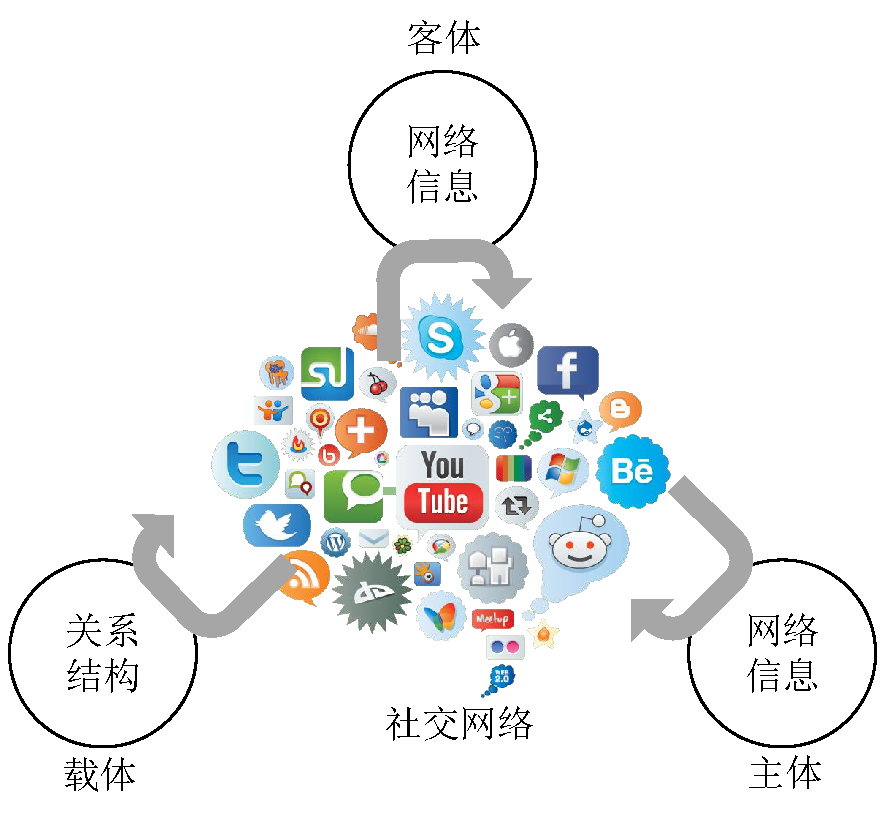
\includegraphics[width=0.5\textwidth]{threeFactors}
    \caption{在线社交网络中的关系结构、网络群体和网络信息}
    \label{fig:threeFactors}
\end{figure}

与传统的Web应用和信息媒体相比,在线社交网络具有如下的新特性:
\begin{itemize}
	\item 高速性:信息发布和接收十分便捷、迅速。社交网络中的用户可以通过手机、笔记本、电脑等终端,随时随地发布和接收信息,信息传递的效率高,具有高速性。
	\item 扩散性:裂变式的信息传播。社交网络中的信息一经发布,便会立刻推送给所有的关注者。信息经过转发,信息又将传播到下一批关注者。信息的传播呈现一种链式反应的几何级数扩散模式,为普通网民传播信息提供了渠道。
	\item 平等性:人人都有可能成为信息输出者。与传统信息媒体中信息发布和信息接收的非对称性相比,社交网络中的每一个参与者都有机会通过社交网络表达自己的观点,传播自己的信息,输出自身的价值观。因此,社交网络在热点事件的产生、发酵、传播等环节中扮演了重要的角色。
	\item 自发性:呈现自媒体形态、自发地形成虚拟社区。社交网络中的个体既是信息的接收者也是信息的发布者,用户会根据自身不同的关注内容与其他用户建立联系,形成网络中的虚拟社区。
\end{itemize}

这些丰富的特性让在线社交网络具有和其他信息媒体不一样的特点,同时也对信息安全提出了新的挑战。对于社交网络分析的研究,在结构、群体以及信息等方面都存在很多已有的工作。其中很多研究工作是关于网络中的信息传播、影响力、传播模型等。这些工作主要研究是否可以建立模型来解释信息的传播方式,如何在真实社交网络信息传播数据集上验证传播模型等等,这些仅仅是社交网络中信息传播研究的一些研究举例。信息传播在实际生活中有着许多应用,例如商业产品或者理念的推广营销、网络流量的爆发检测、寻找关键博客来获取重要的信息、寻找意见领袖或者潮流引领者以及信息的检索排序等等。

社交网络中信息传播关键技术的研究对于理解信息传播的机理有着重要的意义。本文首先在结构上进行理论研究,思考在社交网络中如何选取源节点才能使得信息传播效率更高,提出了传播效率最大化问题。然后,本文在内容方面进行分析,思考社交网络中不同用户的文本内容推送问题。本文利用语言模型以及深度学习等技术,对普通文本信息以及数据流信息进行应用,进行了基于语义扩展和文本质量的实时个性化搜索研究和基于卷积神经网络的文本分类研究,分析不同用户的关注点,将用户所感兴趣的、高质量的信息自动地推送给用户,使得用户更加便捷地获取信息,从而推动信息的传播。最后,本文在传播效果的评估方面进行分析,研究合理的传播模型。本文建立基于概率阅读的传播模型,对于事件的传播影响进行评估,来估测事件传播影响面的大小。本研究对于揭示信息传播的机理和规律、推动社交网络中的信息传播、发现有价值的信息以及保护信息安全起到了重要的作用。

本章首先对本文的研究背景进行阐述,第\ref{sec1:background}小节对在线社交网络中信息传播研究的发展现状进行描述,分析社交网络信息传播分析的研究意义和面临的挑战。其次,第\ref{sec1:relatedWorks}小节对本文研究的各个相关工作进行概述和总结。然后,第\ref{sec1:inovation}小节介绍本文的主要研究内容和创新点。最后,第\ref{sec1:paperStructure}小节给出了本文的组织结构。

\section{研究背景及意义}
\label{sec1:background}
本节主要介绍本文研究的背景及其意义,对涉及到的概念进行详细的阐述,对研究所面临的挑战进行分析。首先,本节对在线社交网络进行一个概述,介绍在线社交网络的起源、定义、特点以及发展状况。其次,本节对社交网络中的信息传播进行介绍,详细地描述信息传播的特点及其所涉及到的因素。然后,本节对本文的研究的意义进行总结。最后,本节分析了研究所面临的挑战。
\subsection{在线社交网络概述}
\label{subsec1:introduction}
人类自诞生以来,就过着群居的生活,一同劳作、交流以及分享,从而形成了社会。随着人类文明的发展和社会的进步,人与人之间的关系进一步的深入和加强,社会关系由简单的血缘关系向朋友关系、雇佣关系以及社交关系发展。而人与人之间由生活、工作、学习、娱乐等等社会交互而形成了某种稳定的关系,这一系列的关系将社会个体结合成了一个巨大的网络,这即是社交网络。如同Linton Freeman所说的那样,我们都被一个无形的网络连接在一起\upcite{freeman2004development}。

社交网络(Social Network)在维基百科中被定义为由社会个体(例如个人或者机构等)、社会个体间的二元关系以及社会个体之间的社交互动组成的社会结构\upcite{social_network}。在社交网络中,个体之间因为社交互动而形成相对稳定的关系体系,这种关系可能是亲属关系、朋友关系、同学关系,也可能是商业合作关系或者宗教信仰关系等。通过这些关系,社交网络把偶然相识的弱关系到紧密结合的强关系,以及社会中各式各样的人群串联成了一张巨大的网络。由于社交网络中存在各种各样的社会关系,个体之间的网络结构往往是非常复杂的。而且,复杂的关系结构也会影响网络中个体之间的社交互动,进而影响到个体的社会行为。

随着工业化、城市化的进行以及移动网络的发展,社会网络化的趋势日益凸显。在2012年,Lee Rainie和Barry Wellman在其著作《网络化:新的社会操作系统》\upcite{rainie2012networked}中指出,社会网络革命、移动革命以及互联网革命将是影响人类社会发展的三大革命。随着互联网的进步,网络结构受地域性因素的影响减弱了,这使得跨地域性的线上社会关系成为了社交网络的主要形式。在现实社会中,人们相继在社交媒体平台上创建账号,将线下的社会关系扩展到了线上,并且进一步的延伸,这使得在线社交网络成为了人们网络生活中不可或缺的沟通工具。

在2009年欧盟关于社会计算的研究报告中\upcite{huijboom2009key},在线社交网络主要可以分成如下的四个大类,
\begin{itemize}
	\item 即时通讯应用。这一类的应用提供一个实时的通信平台,使得人与人之间能够通过网络进行在线的交流、信息的分享等。典型的代表有MSN、QQ、飞信等,其具有双向认证与实时推送的特点。
	\item 在线社交应用。这一类的应用提供一个在线社交关系平台,人们在平台上进行社交互动以及消息的共享等。典型的代表有脸书(Facebook)、谷歌+(Google+)、人人网、QQ空间等,其具有双向认证以及非实时推送的特点。
	\item 微博类型应用。这一类的应用提供一个自媒体的信息发布平台,任何个人或者机构都能在平台上发布信息,推送给其关注者。典型的代表有推特(Twitter)、新浪微博、腾讯微博等,其具有单向认证以及实时推送的特点。
	\item 共享空间以及其他应用。这一类的应用提供一个公告发布系统,具有沟通功能,但是用户之间结合不紧密。典型的代表有BBS、论坛、博客等,其具有单向认证以及非实时推送的特点。
\end{itemize}

社交网络是Web 2.0时代的具有代表性的应用,具备Web 2.0时代交互性、主动性的特点,众多社交软件应用随着技术的更新而蓬勃发展。中国流行的即时通信软件“腾讯QQ”诞生于1999年,在2016年的月活跃账户数(MAU)达到8.77亿,其中智能终端月活跃账户达到6.47亿\upcite{tencentReport2016}。2004年于美国上线的社交网络服务网站脸书(Facebook)成为了全球范围内最流行的社交网站之一。从网站成立至今,其用户持续增长,在2016年第四季度,脸书月活跃人数已经突破了18.6亿,其中移动端用户数达到了17.4亿\upcite{facebookReport2016}。2006年微博客类的应用推特(Twitter)在美国诞生,允许用户更新不超过140个字符的消息,成为一个广受欢迎的社交网络及微博客服务网站。截至2016年第四季度,推特的平均月活跃用户为3.19亿\upcite{twitterReport2016}。随着全球社交网络的发展,相似的网站在国内也纷纷出现。2009年,新浪微博正式上线,政府、明星以及草根用户等社会各界人士纷纷开设账户,发布和接收信息。截至2016年底,新浪微博的月活跃用户数达到了2.97亿,其中89\%的用户为移动端用户,平均日活跃用户(DAU)达到了1.32亿\upcite{weiboReport2016}。腾讯在2011年推出的一个为智能终端提供即时通讯服务的软件“微信”在当今已经成为了新时代移动端即时通讯的领军,微信和WeChat(微信的海外版)在2016年的合并月活跃账户数达到8.46亿\upcite{tencentReport2016}。

随着网络科技和设备产品的飞速发展,社交网络逐渐成为人们接收传播信息、发表自身观点以及讨论公共事件的主要渠道。根据中国互联网络信息中心(CNNIC)发布的第39次《中国互联网络发展状况统计报告》显示,截至2016年底,中国网民的规模达到了7.31亿,与欧洲的人口总量相当,互联网的普及率达到了53.2\%。其中手机网民占比达到了75.1\%,规模达到6.95亿,增长率连续三年超过10\%,移动互联网极大地丰富了网民获取信息的通道\upcite{cnnic2017zghlwfzbg}。随着网民数量的增长,社交网络中的信息量也随之上升。推特中每天产生的信息突破了0.58亿条,查询次数突破了21亿次\upcite{statisticbrain2017twitter}。脸书平均每20分钟就有1百万条链接被分享、3百万条信息发布\upcite{statisticbrain2017facebook}。2017年的春晚直播期间,在新浪微博平台中讨论春晚的微博数量达到了近6千万条,网友互动量达1.99亿次,共有超过1.2亿网友参与到了微博抢红包的活动中\upcite{techsina2017newyear}。2017年的除夕,国人在微信和QQ平台上使用红包互送祝福,其移动支付峰值达到了20.8万笔/秒,合计支付总数达到了32.2亿笔\upcite{techqq2017luckymoney}。由以上数据可以看出,社交网络为人们生活的各方面都提供了平台,成为了人们获取、发布以及传播信息的关键渠道。

社交网络之所以能够如此迅速的流行起来,是因为它具有如下一些特点。首先是社交网络简单易用。任何个人或者组织都能够随时随地发表言论,分享内容。而且,用户接收和发布信息的渠道多种多样,可以在互联网的客户端,也可以在移动客户端。这些都极大地加速用户接收、发布和传播信息的速率,使得信息在群体之间的传播更加的高频化。其次是社交网络交互频繁。社会个体通过关注/被关注、好友等关系紧密联系在一起,网络结构复杂。群体之间通过兴趣爱好、共同关注点等因素形成较为固定的社区,社区内部的成员在同一个话题上相互讨论、分享。与传统信息媒体不同,社交网络中的社会个体既是信息的接收者,又是信息的传播者,同时还可能是信息的传播者。这些因素都促进了社交网络中信息的产生与传播。然后是社交网络与现实社会相互映射。随着社交网络的发展,越来越多的个人和机构在社交网络中实名认证,在网络世界中与人们交互来提高自身的影响力。这进一步地拉近了虚拟和现实之间的差距,真实社会中发生的事件将会迅速的在社交网络中以信息的形式发布与传播。

由于上述的原因,社交网络迅速崛起,在短时间内吸引了大量的用户加入。用户在社交网络中分享现实社会中发生的事件,发表自己的意见,这也使得虚拟网络和现实世界的界线逐渐模糊。由于网络资源的公开性以及透明性,社交网络中的数据相对于现实世界要易于获取,这使得一些原本在现实世界中难以研究的内容存在了研究的可行性。研究者可以分析虚拟网络中的数据,并通过现实世界在虚拟网络中的映射,间接来研究现实世界中的问题。例如人口年龄分布问题、政策满意度问题、舆论热点分析等等都可以在社交网络中得到较好的解决。正因如此,社交网络的出现促进了社会学、传播学、系统科学、计算机科学等学科新一轮的发展。

\subsection{社交网络信息传播}
\label{subsec1:informationDiffusion}
在线社交网络与生俱来的自由性和开放性,使其成为了现代社会中信息传播的重要渠道,社交网络中的信息传播活跃度达到了前所未有的程度。信息传播(Information Diffusion)是指个体、组织之间的信息传递和交流\upcite{baike2017info}。人们通过符号、信号等信息载体来接收、传递与反馈信息的活动,人们相互交换思想和意见等,以达到相互影响和了解的过程。而社交网络信息传播指的是以社交网络为媒介进行信息传播的过程\upcite{方滨兴2014在线社交网络分析}。1948年,Lasswell在《社会传播的结构与功能》\upcite{lasswell1948structure}一文中指出了传播过程及其“5W”要素,即:谁(Who),说了什么(Says What),通过何种渠道(In Which Channel),对谁(To Whom),造成了什么结果(With What Effect)。经典的5W传播模式构成了传播学中研究的五个基本内容,即控制研究、内容分析、媒介研究、受众研究以及效果研究。

社交网络信息传播影响着生活的各方各面,并且改变人们的行为模式。2007年,Christakis和Fowler在新英格兰医学杂志上的发表文章\upcite{christakis2007spread},研究分析了12,000名患者的药物记录,并根据患者之间的亲属关系、邻居关系等,从药物记录中抽取了一个离线的社交网络。研究的目的是分析非传染病(例如肥胖症等)与患者社交网络邻居的关系,理解具有患非传染病网络邻居和自身患有该非传染病的关联关系。在不考虑其他原因的情况下,研究表明拥有肥胖症患者朋友会使得自身也患肥胖症的风险提高171\%。这说明了肥胖症患者会通过社交网络把容易导致肥胖的习惯传播给其网络邻居。该研究主要把重点放在了关联关系上,而不是患病原因,研究结果表明了社交网络间传播影响的效应。在Christakis和Fowler的另一个研究中,吸烟这一个行为也在社交网络中的传播影响也得到了印证\upcite{christakis2008collective}。在2011年,Christakis和Fowler在其著作\upcite{christakis2009connected}中指出了传播的重大影响,并解释了社交网络的组成和运作机理。其中包含了很多真实的案例,例如背痛的症状自柏林墙推倒后从西德传入东德,自杀倾向通过社团传播,政治倾向和信仰通过网络传播等。而在商业圈,信息传播引领成功的最为著名的案例是“Hotmail现象”\upcite{hugo2001emergence}。在20世纪90年代初,Hotmail是一个相对冷门的邮件服务提供商。为了改变这个局面,公司使用了一个相对简单的创意,即在每一封用户发送的邮件结尾自动地加上“欢迎加入世界上最大的邮件服务提供商MSN Hotmail”这一宣传语。这一宣传语通过用户之间的邮件传播,加速了品牌的树立和传播。在短短18个月后,Hotmail就成了世界第一大邮件服务提供商,拥有了800万用户。在2012年7月发布的一首韩国流行歌曲“江南style”成为了YouTube上最先突破10亿观看的节目。而在另一方面,社交网络中的信息传播在社会的突发事件中也有着体现。在2011年夏天,加拿大温哥华举办的史丹利杯冰球决赛引发了骚乱。其中许多是青少年,他们破坏了城镇中的财物,并且在社交媒体上自吹自擂,例如发布图片、视频等。这引发了广泛的传播,并且成为了法庭的取证。相比于现场的证据,社交媒体中的证据种类更多。这使得警方在短时间内确认了骚乱者的身份。

社交网络中的信息传播具有以下特点。首先,社交网络中的信息发布与接收十分便捷、快速,用户可以通过手机等移动设备随时随地发布和接收信息。其次,社交网络中的信息传播的扩散形式呈“裂变式”扩散。消息一经发布将即刻推送到关注者,而关注者的转发将产生下一轮的传播。然后,社交网络中的每一个用户都有成为意见领袖,热点制造者的可能,所有网民都可能在热门事件的传播中扮演重要的角色。最后,社交网络中的信息传播呈现“自媒体性”,任何一个用户或者机构都能够建立属于自己的媒体,通过发布信息、制造热点、传播信息来扩大自身的影响力。这些特点使得社交网络中的信息传播更加迅捷、传播范围更广,人们在社交网络中的交互更加的频繁。

社交网络信息传播之所以有如上的特点是由于如下几个因素\upcite{方滨兴2014在线社交网络分析}。首先是关系结构。社交网络中的个体基于相互认识、兴趣爱好或是个人崇拜等原因,在社交网络上形成了复杂的关系结构。其次是网络群体。基于社交网络中的关系结构,网络个体因为关系而大量聚合,并且相互作用、相互影响,从而形成具有不同特征的网络群体。最后是网络信息。社交网络中的关系结构提供了底层的高速传播通道,网络群体直接助力网络信息的传播,丰富的网络内容提供了信息资源。关系结构、网络群体以及网络信息的有机结合加速了网络信息的传播。

\begin{itemize}
	\item 网络结构。社交网络中的个体间进行丰富的交互,形成了“一对一”、“一对多”、“多对多”以及“多对一”几种传播模式的组合。网络结构中节点间的连接强度和网络密度各不相同,从而形成了不同的连接关系。强连接会导致形成紧密联系、聚集的社区结构,意见更加统一;弱连接通常在关系不紧密、联系不频繁的个体间形成,可以提供新的信息,丰富了信息的内容,扩大了传播范围。
	\item 网络群体。网络个体聚合并且相互影响、形成了网络群体。与现实世界中的群体相比、网络群体传播具有高度的互动性、开放性、跨地域性等特点。网络群体中的意见领袖往往具有较大的影响力,能够引领其所在群体对于事件的倾向性和态度。
	\item 网络信息。网络信息具有时效性、多源性、多样性等特点,在信息传播时起着不可或缺的作用。社交网络的信息的源头不仅仅是网络中的链接信息,而且来自于传统媒体的信息接入。网络信息在社交网络中传播会产生相互影响,与独立信息的传播不同,可能引发更多的讨论和演化。
\end{itemize}

社交网络信息传播由于这些新的因素的出现,凸显出与传统信息传播的不同特性,加速了信息传播的效率和多样化。在实际生活中影响到人们的各方各面,在给人们带来巨大便利的同时,也对信息安全提出了新的挑战。
\subsection{研究意义}
\label{subsec1:researchSignificance}
研究社交网络中信息传播对科学研究、社会安全以及商业发展都是十分有意义的。研究社交网络中的信息传播规律,有助于加深我们对于社交媒体的理解,解释社会中发生的现象,同时使得我们对于复杂的网络拓扑结构、传播能力以及网络动力学等有着进一步的认识。

从科学研究的角度来讲,研究社交网络中的信息传播更有益于理解信息的传播机理,方便推动或者干预信息在人类社会的传播。随着社交网络的发展,各类社交媒体的兴起,用户在网络上发布信息的数量呈爆炸式增长,这些信息通过社交网络这一个良好的渠道在用户之间迅速传播。社会中的事件都会在网络中得到体现,用户将分享个人的生活、讨论热点事件、发表政治观点等等。社交媒体中的信息量已经逐渐超越了传统的新闻、博客等应用的信息量,社交网络成为了信息传播的主要平台。信息在传统的媒体中传播往往通过线上线下的口口相传等途径,而这些方式难以形成记录。社交网络中的信息传播有迹可循,能够记录其传播轨迹,这为开展相关研究提供了丰富的数据基础,使得研究人员有机会在海量的真实数据上建立模型,研究信息传播机制,认识传播规律。

从社会安全的角度来讲,研究社交网络中的信息传播能够使得人们及时接收到真实的信息,免受谣言的危害,保护社会公众的安全与财产。社交网络融入了人们的日常生活,改变了人们的生活方式,影响到包括政治、教育、经济、文化等等方面。在政治方面,微博已经直接在很多政务活动中发挥了巨大的作用。在2008年的美国大选中,奥巴马及其团队利用社交媒体推特进行了助选活动,在推特上制造舆论,争取选票。奥巴马接受竞选总统提名的演讲创下了推特每分钟发表推文5.2万条的记录。在当选之后,奥巴马及其团队继续利用社交网络提高政治影响力。在教育方面,美国的众多大学纷纷在社交网络上发布公开课,直接支持远程教育,并且在脸书和推特上与慕课(MOOC)进行资源整合。在经济方面,电子商务已经成了人们的主流购物方式之一。众多的公司通过社交网络进行宣传,提升自身品牌的竞争力,最终提高了营业额。在文化方面,社交网络正在改变人们的生活方式,足不出户便能与世界各地的网友进行互动,直播平台、虚拟现实技术的诞生使得人们的交互体验更加的多样化。与此同时,社交网络中的信息传播也会给社会带来负面影响。在政治方面,不法分子蓄意制造和传播有害国家安全和社会利益的谣言,影响社会稳定。我们民众曾多次受到微博谣言的影响而发生“抢盐”风波。在教育方面,邪恶势力通过社交网络蛊惑青少年崇尚暴力,灌输错误思想,怂恿其破坏社会的稳定。在经济方面,网络诈骗者利用社交网络发布虚假信息,进行诈骗活动,损害人们的经济利益。在文化方面,犯罪团伙利用社交网络,传播网络色情以及暴力信息,而且往往伴随着传播网络病毒、木马等行为。

在商业发展的角度来讲,研究社交网络中的信息传播能够使得个人、公司或者组织抓住机遇和挑战,实现自身利益的最大化。个人通过社交媒体发布自己的观点、看法,成为社交网络中的意见领袖,形成自媒体。社交网络使得推广自己更加的便捷、简单。例如,罗振宇在社交网络中推广“罗辑思维”节目而走红,成为了自媒体“首富”。而互联网企业通过分析社交网络中的趋势,制定自身的战略方向,通过社交网络发布自己的产品或者理念,能够快速地推广自身的产品。同时,社交网络中的个人信息透明化,使得个人隐私更容易被利用,这对隐私保护提出了新的要求。社交网络中信息传播速率快,传播范围广,这对企业的公关能力提出了挑战。

综上所述,社交网络的发展对社会各方各面都带来了机遇和挑战,同时也对人们提出了新的要求。研究社交网络信息传播有助于理解传播的机理,提高应对突发事件的能力,促进经济的繁荣发展,对于政治经济安全、国家社会稳定以及企业个人财产利益都有着重要的意义。
\subsection{面临的挑战}
\label{subsec1:challenge}
在线社交网络中信息传播分析与自然语言处理、数据挖掘、机器学习、海量数据处理、传播学、社会学等等学科有着紧密的联系。社交网络带来了丰富的语料数据和结构关系,但是也提出了新的挑战。尽管与之相关的各个领域的研究已经取得了很多的成果,提供了相应的技术支持。但是,由于在线社交网络中的信息传播同以往的研究存在诸多不同之处,这一研究依然面临着新的问题与挑战,具体包括如下几个方面。

\begin{itemize}
	\item 数据的海量性。社交网络信息传播分析所涉及到的数据量往往是海量的,这对信息传播的分析提出了较大的挑战。数据的海量性体现在两个方面,一个是信息内容海量,二是用户结构海量。这对信息传播的分析算法处理数据的能力提出了新的要求。在一些热点突发事件的爆发过程中,社交网络中的信息往往在短时间内便会达到一个较大的数量级,例如2016年奥运会中的中国女排夺冠,“女排精神”成为了国人共同的关注点,女排夺冠相关内容互动量在当天达到了7285万次,相关视频播放量达到3.4亿次\upcite{sina2016volleyball}。信息传播分析通常需要分析文本的内容,分析用户之间的传播关系等,如何实时地处理如此庞大的数据是社交网络信息传播需要研究的问题。
	\item 文本的多样性。社交网络中的文本形式多样,微博类的应用通常限定用户的文本长度不超过140个字符。而新闻、论坛或者微博中的长博文则对用户发表文本的长度没有严格的限制。这使得传统的文本表示模型在社交网络中,对长短文本的处理性能明显下降,在文本分类、文本聚类、信息推荐等应用方面影响较大。因此,社交网络中的信息该如何表示对社交网络中信息检索、信息推荐等应用提出了新的挑战。
	\item 结构的复杂性。社交网络中的用户数量庞大,而且不同社交媒体之间的用户存在着重叠现象。社交网络中的用户通过朋友、兴趣等多种关系聚合在一起,形成多种多样的复杂结构。计算信息传播的影响范围、信息的溯源以及如何选择节点使得影响力最大化这些问题在社交网络环境中都出现了新的挑战,传统的方法的性能在复杂的网络中效率明显下降。如何在复杂的网络中快速地、有效地对信息传播进行分析对抽样理论、算法设计等都提出了挑战。
\end{itemize}

由此可见,社交网络的发展对信息传播研究提出了多方面的挑战,同时,也为信息传播研究提供了丰富的数据和渠道,这也为信息传播的研究提供了一个虚拟的环境。

\section{相关研究工作}
\label{sec1:relatedWorks}
社交网络中的信息传播相关的工作涉及到的研究十分广泛,包括自然语言处理、数据挖掘以及机器学习的各种研究方法。本小节主要从传播源的选择、信息内容的选择以及传播效果的评估等方面介绍相关的研究工作。其中涉及到的相关工作有影响力最大化、实时个性搜索、语言模型与文本分类以及传播模型的学习等相关研究。
\subsection{影响力最大化}
\label{subsec1:influenceMax}
影响力最大化问题的实际应用是通过信息传播来推广新产品、新理念以及新政策等。为了实现网络中信息的迅速传播,主要有研究分为两个方向。第一个方向是传播模型的建模,第二个方向是寻找一个快速有效的方法来找到具有影响力的个体。

对于第一个方向,已有很多工作对传播模型进行了深入的研究。均匀模型(Uniform Model)假设所有节点的影响概率为一个常数(例如0.01),该模型不区分节点之间的关系。首先,每一个节点都以相同的概率影响其邻居节点,模型未能区分节点对于其他节点的影响力。其次,每一个节点受到其邻居节点的概率也是相同的,模型未能区分不同邻居节点对该节点的影响力。显然,这样的假设是值得商榷的。三态模型( Trivalency Model)在一定程度上解决了第一个问题,节点的影响概率为一个集合中的某一个元素,例如$\left\{ 0.001, 0.01, 0.1\right\}$。模型的思想是对不同影响力的节点赋予不同的影响概率值。上述的两个模型的影响概率与网络的结构无关。在加权级联模型(Weighted Cascade Model)中,模型定义影响概率与网络的边$\left(u,v\right)$相关,影响概率$p_{uv}=1/d_{in}v$,其中$d_{in}v$为节点$v$的入度。该模型比均匀模型和三态模型拥有更好的性质。首先,低入度的节点受到其入度邻居节点的影响要大于高入度的节点。这样影响概率不仅仅是从一组常数中进行选择。其次,一个节点对于出度节点的影响不再是相同的,这是由于这些出度节点的入度不同。然而,加权级联模型仍然无法解释节点之间的影响概率是如何计算得出的。Saito等人\upcite{saito2008prediction}研究了如何学习影响概率的问题,主要以独立几联模型为研究对象。通过观测信息传播过程中的每个时间段,来求解设定影响概率为参数下的极大似然估计,从而求解影响概率。在线性阈值模型中,每个节点存在一个阈值$\theta \in \left[ 0,1 \right]$,当累计影响超过阈值时,节点将被激活。Goyal等人\upcite{goyal2010learning}通过社交网络中的信息传播轨迹来学习节点之间的影响概率。

对于第二个方向,影响力最大化问题最早是由Domingos和Richardson所提出,问题基于马尔科夫随机场(Markov Random Field)进行建模\upcite{domingos2001mining,richardson2002mining}。随后,Kempe等人将影响力最大化问题建模成一个离散的随机优化问题\upcite{kempe2003maximizing}。影响力最大化的问题可以定义为如下所示,

\begin{defn}[影响力最大化问题]
\label{def:imProblem}
影响力最大化问题可以形式化为如下一个随机优化问题:给定一个图$\mathcal{G} = \left(\mathcal{V}, \mathcal{E}\right)$、图$\mathcal{G}$上的一个随机传播模型以及一个阈值$k$。给定一个种子节点集合$S \subseteq \mathcal{V}$且满足$\left\vert{S}\right\vert \leq k$,则集合$S$的影响力期望为$\mathbb{E}_\mathcal{G}\left[I\left(S\right)\right]$。则影响力最大化问题为寻找使得影响力期望最大的集合$S^{\ast}$。问题可表示为如下所示,
\begin{equation}
\label{eq:imProblem}
    \begin{split}
        &S^{\ast} = \arg\max{\mathbb{E}_\mathcal{G}\left[I\left(S\right)\right]}\\
        &s.t.~~S \subseteq \mathcal{V},\left\vert{S}\right\vert \leq k
    \end{split}
\end{equation}
\end{defn}

在给定了一个传播模型后,例如独立级联模型(Independent Cascade Model)或者线性阈值模型(Linear Threshold Model),影响力最大化问题可以分解成两个问题。第一个问题称为影响力期望计算问题,即给定了一个种子节点集合$S$后计算其影响力期望$\mathbb{E}_\mathcal{G}\left[I\left(S\right)\right]$。第二个问题是如同定义\ref{def:imProblem}所示,找到使得影响力期望最大的种子节点集合。

对于影响力期望计算问题,Wang等人\upcite{wang2012scalable}以及Chen等人\upcite{chen2010scalableLT}证明了其复杂度在独立级联模型和线性阈值模型下是\#P-难的。\#P问题是计数问题,与NP问题中决策问题相关。NP问题需要求解一个问题实例是否存在解,例如合取范式(Conjunctive Normal Form)方程是否存在可满足解,而\#P问题需要求解这个问题实例存在多少个解,例如合取范式方程存在多少个可满足解。如果一个问题是\#P的且每一个\#P的问题都可以在多项式时间内归约到它,那么这个问题是\#P-完全的。如果一个问题可以在多项式时间内由一个\#P-完全的问题归约到它,那么它是一个\#P-难的问题。对于独立级联模型或者线性阈值模型,上述的证明过程都可以由一个\#P-完全的问题,$s$-$t$连通性问题\upcite{valiant1979complexity},来进行归约。

对于寻找影响力期望最大的种子节点集合的问题,Kempe等人\upcite{kempe2003maximizing}给出了结论,问题的复杂性在独立级联模型和线性阈值模型下都是NP-难的。其证明思路将NP-完全的问题归约到影响力最大化问题。在独立级联模型中,证明将子集覆盖(Set Cover)问题归约到影响力最大化问题;而在线性阈值模型中,证明将节点覆盖(Vertex Cover)问题归约到影响力最大化问题。

上述研究表明了影响力最大化问题是一个复杂性较高的问题。问题的难度来自于两方面,一方面是问题的组合性质,另一方面是计算影响力期望的难度(甚至是计算一个节点的影响力期望)。针对这两个问题,已有的研究主要应用贪心算法来解决组合问题,利用蒙特卡罗(Monte Carlo)模拟来解决影响力期望计算问题。对于影响力最大化问题使用贪心算法能够得到一个下界的保证,即运用贪心算法得到的解最差的结果有理论性的保证。这是由于影响力期望函数$\mathbb{E}_\mathcal{G}\left[I\left(\cdot\right)\right]$具有两个很重要的性质,即子模性(submodularity)和单调性(monotonicity)。子模性的定义如下所示,
\begin{defn}[子模性]
\label{def:submodularity}
子模性的定义可以解释为往种子节点集合加入更多节点时,所造成的效果为边际收益递减(Diminishing Marginal Returns)。对于一个集合函数$f:2^{\mathcal{V}} \rightarrow \mathbb{R}$,如果对于任意的子集$S \subseteq W \subseteq \mathcal{V}$且任意的元素$v \in \mathcal{V} \setminus W$,将元素$v$加入到集合$W$中的边际收益不超过将元素$v$加入到集合$S$中的边际收益,那么函数$f\left( \cdot \right)$具有子模性,用公式表示如下,
\begin{equation}
\label{eq:submodularity}
	f\left(S\cup\left\{v\right\}\right) - f\left(S\right) \geq f\left(W\cup\left\{v\right\}\right) - f\left(W\right)
\end{equation}
\end{defn}

另一个重要的性质单调性定义如下,
\begin{defn}[单调性]
\label{def:monotonicity}
单调性的定义可以解释为往集合中增加元素不会使得函数值变小。一个集合函数$f:2^{\mathcal{V}} \rightarrow \mathbb{R}$,如果对于任意的子集$S \subseteq W \subseteq \mathcal{V}$,都有$f\left(S\right) \leq f\left(W\right)$,则函数$f\left( \cdot \right)$具有单调性。
\end{defn}

对于具有子模性和单调性的函数$f\left( \cdot \right)$,Nemhauser等人\upcite{nemhauser1978analysis}证明了使用贪心算法得到的解的性能存在着下界。令$S^{\ast}$表示问题的最优解,函数$f\left( \cdot \right)$具有子模性和单调性且满足$f\left( \emptyset \right) = 0$,$S^g$为通过贪心算法得出的解,则可以用公式表示为如下所示,
\begin{equation}
\label{eq:lowerBound}
	f\left( S^g \right) \geq \left( 1 - 1/\mathsf{e} \right) f\left( S^{\ast} \right)
\end{equation}
其中$\mathsf{e}$为自然对数的底。其证明过程\upcite{chen2013information}利用了单调性和子模性以及递推方法得到公式(\ref{eq:lowerBound})的结论。

对于影响力最大化的求解,Kempe等人\upcite{kempe2003maximizing}的研究是最早将影响力最大化问题当做优化问题来求解的,并且给出了贪心算法的求解。Leskovec等人\upcite{leskovec2007cost}提出了一种改进算法,CELF算法。算法利用函数的子模性来对于不必要的模拟进行剪枝,使用一个优先队列实现,在不改变输出的情况下提高了算法的性能。Goyal等人\upcite{goyal2011celf++}基于上述的工作进行了改进,提出了CELF++算法。Cheng等人为了解决可扩展性和准确度之间的矛盾,提出了一个静态的贪心算法,为StaticGreedy算法。该算法保证了信息传播过程中影响函数的子模性,在准确度不损失的情况下,极大地降低了运算量。Borgs等人提出了一种不同于贪心算法的新型框架,利用了反向传播抽样方法,极大地加速了算法的效率,同时保证了算法的性能。

基于影响力最大化问题,许多研究提出了基于此之上的衍生问题。传统的影响力最大化问题是种子节点集合的大小进行限制,阈值为$k$。Leskovec等人\upcite{leskovec2007cost}假设选择每一个节点都会产生开销,每一个节点的开销不尽相同,而总开销的大小固定作为限制,问题是在不超过总的预算下来产生最大的影响。在某些情况下,网络可能是动态的网络,在动态网络中研究影响力最大化问题\upcite{chen2015influential,zhuang2013influence}也是一个十分有意义的方向。Yang等人\upcite{yang2016continuous}对动态的影响力最大化问题进行研究,提出了一种通用的坐标下降算法来解决该问题。Wang等人\upcite{wang2015maximizing}在原问题的基础上,考虑了激活的节点以及最终传播到单未激活的节点(称之为已通知的节点)两类节点,提出了信息覆盖最大化问题(Information Coverage Maximization),并对该问题进行了求解。Liu等人\upcite{liu2012time}将传播时间纳入了考虑,提出了一种时间约束的影响力最大化问题。Shishir等人\upcite{bharathi2007competitive}考虑到了信息传播中多个传播源博弈游戏,对多源情况下的信息竞争传播问题进行了分析,对先手情况给出了求解方法。

\subsection{实时个性化搜索}
\label{subsec1:realTimeSearch}
实时个性化搜索的目的是根据用户偏好迅速地识别出用户所感兴趣的物品或者内容,涉及到许多的研究领域,包括个性化搜索、语言模型以及协同过滤等等。

在个性化搜索方面,根据不同的用户,对于检索内容进行重新排序是提高性能的一个常用的方法。Xie等人\upcite{xie2016personalized}针对上下文关系中的语言知识,使用图结构对语言知识的内容和相互关系建模,从而获取用户的偏好。同时,该工作提出了一个发现支配集的算法,来降低非相关上下文的影响,并提出了一个重排算法来衡量一次查询与信息的相关性、发现的文本内容与用户信息的相关性。Sontag等人\upcite{sontag2012probabilistic}针对特定用户的个性化搜索提出了一个新的方法。工作提出了一个关联生成模型,可以用来针对一次查询计算文本和用户的关联。生成模型中的用户相关的参数构成了一个用户的信息,可以通过用户长期的搜索记录来进行学习。Wang等人\upcite{wang2013personalized}针对搜索引擎对用户不区分的问题,提出了一种通用排序模型的适应性框架来解决个性化搜索问题。模型使用一个离线训练的用户无关的排序模型以及有限数量的不同用户的查询,能够更好的适应不同用户的搜索偏好。Tang等人\upcite{tang2015personalized}将个性化推荐问题形式化为一个上下文歹徒问题(\textit{contextual bandit problem}),来解决获取新的知识和基于已有知识做决策的相互制约问题。工作提出了一种非参数的策略,使用了一个有规则的重采样方法来得到需要估测模型的分布。根据概率匹配的模式,算法随机地从得到的分布中选取一个模型。Leginus等人\upcite{leginus2016personalized}针对推特中信息量繁多,而用户无法处理大量信息的问题,提出了个性词语云生成的方法来作为用户导航。用户的行为历史,例如发布的推文、转推、浏览的推文,都可用来提升词语云的个性化。Du等人\upcite{du2016folksonomy}对协同标签系统中个性化搜索中的用户建模进行了研究,通过标签以及排序等信息,提出了一种多层次的用户模型,实现个性化搜索。模型不仅能够反应出用户的偏好,也能反应出用户不喜欢的内容。Younus等人\upcite{younus2014language}针对个性化搜索引擎中的用户模型进行了研究,利用推特作为个性化搜索引擎的用户信息源,提出了一种统计语言模型,将推特中的用户特征考虑在内。个人化的用户模型使得检索的准确率得到了显著的提高。Xie等人\upcite{xie2014mining}针对社交网络中隐藏用户社区发现问题进行了研究,提出了增强分类图(Augmented Folksonomy Graph)的机制来包含社交网络中的多方面关系,同时基于一种新型的密度估计的聚类方法来寻找隐藏的用户社区。Li等人\upcite{li2015real}针对社交网络中的频繁信息更新以及小世界特性,提出了一种通用框架来解决个性化top-k查询问题。框架基于通用的排序框架,集成了时间新鲜度、社交相关性以及文本相似度特征。算法应用了一个三维立方倒排索引来支持在三个特征维度上有效的剪枝。然后提出了一个基于该立方的算法来检索top-k的结果。

在短文本的研究方面,由于社交网络中的文本具有不同的性质,包含了更多的标签以及结构化和非结构化的属性,因此对这方面的研究是十分有必要的。在社交网络中的信息检索方面,Massoudi等人\upcite{massoudi2011incorporating}为了解决社交网络中短文本信息量不足的问题,提出了一种检索模型,对特定话题检索微博中的博文信息。由于传统的信息检索模型在微博中无法直接适用,研究针对微博的特性设计了一种语言模型。算法通过文本特性和微博特性两方面对模型的性能进行提升,同时使用了一个动态的查询扩展模型来对微博博文检索进行处理。Severyn等人\upcite{severyn2015learning}使用了卷积神经网络来重排短文本对(查询-文档对),其中神经网络可以用来表示短文本对以及计算他们之间的相似度。该算法将词语当做输入,简化了预处理过程。该方法在TREC的两个常见的任务(智能问答以及微博检索)中显示了较好的性能。Ren等人\upcite{ren2014hierarchical}在社交网络流数据中的层次多标签的分类中进行了研究,由于概念漂移、种类之间的复杂关系以及社交网络数据流中的文本长度有限对该问题都提出了挑战。研究的核心思想包括短文本的扩展、时间感知的话题追踪和基于块结构的学习。Paik\upcite{paik2013novel}对信息检索中的词语权重问题进行了研究,提出了一种新型的tf-idf词语权重方法。算法使用了两种不同的文档词频归一化来得到两方面的词语特性。一种词频在短文本中效果较好,另一种在长文本中效果较好,最终的词语权重综合考虑了这两部分的影响。

在协同过滤搜索方面,由于社交网络中的信息和用户紧密相连,优质的用户更可能产生有意义的信息。Xue等人\upcite{xue2009user}针对传统搜索中两个主要问题,数据稀疏性以及新用户的冷启动,提出了协同个性化搜索的方法。该方法不仅考虑了特定用户群和全局用户之间的共性,并且考虑了个体的特性。方法建立一个统计用户语言模型来结合个人模型,用户群模型以及全局用户模型。Vosecky等人\upcite{vosecky2014collaborative}针对微博领域内协同搜索的不足,针对推特中的协同个性化搜索提出了一种新型的框架。算法的核心是一个协同用户模型,该模型用来表示用户的社交连接,从而获取用户更全面的偏好。

\subsection{语言模型与文本分类}
\label{subsec1:textClassification}
语言模型是研究文本的基础,包括特征提取、特征权重以及语义相似度计算等。特征提取研究的是选取哪些特征来表示文本的问题,特征权重以及语义相似度计算则是计算问题。特征选择存在许多不同的方法,可以采用词语、短语等作为特征,也可以采用n-gram模型选择特征项,也可以采用知识库中的概念作为特征项。

布尔模型\upcite{salton1975vector}是在文本信息检索中的一种简单的模式,该模型是特征项的严格匹配。每一个特征项的取值都有True和False两种取值,其中True表示文本中存在该特征,False表示不存在。用户的查询采用逻辑运算来表示特征项之间的关系,文本的匹配查询过程则是布尔逻辑运算。该模型的优点是运算速度快,可以表示一定的逻辑关系。但是该模型也存在明显的缺陷,首先是无法对特征值的重要性进行赋值,且缺乏定量的分析。用户在进行查询的时候需要自己构建复杂的查询表达式。查询的结果仅有命中和不命中两种结果,适用范围较小。

向量空间模型(Vector Space Model)是另一种类型的模型。在这个模型中,特征项是代表着向量空间中不同的维度,文本则可表示为该空间中的一个向量,向量中每一个维度的分量可以使用词频、tf-idf值等。例如选择tf-idf值作为分量时,一篇文档$\mathbf{d} \in \mathbf{D}$可以表示为如下,
\begin{equation}
\label{eq:documentVec}
	\mathbf{d} = \left({tfidf}_{1,\mathbf{d}}, {tfidf}_{2,\mathbf{d}}, \cdots, {tfidf}_{N,\mathbf{d}}\right)
\end{equation}
其中${tfidf}_{i,\mathbf{d}}$表示特征项$i$的tf-idf值,$N$为特征的总数。tf-idf值的计算公式如下所示,
\begin{equation}
\label{eq:tfidfFormula}
	{tfidf}_{i,\mathbf{d}} = {tf}_{i,\mathbf{d}} \cdot {idf}_i = \frac{n_{i,\mathbf{d}}}{\sum_j n_{j,\mathbf{d}}} \cdot \log{\frac{|D|}{1 + \vert \{\mathbf{d} \in \mathbf{D} : i \in \mathbf{d}\}\vert}} 
\end{equation}
其中${tf}_{i,\mathbf{d}}$表示特征$i$在文档$\mathbf{d}$中的频率,${idf}_i$表示特征$i$的逆向文件频率,$n_{i,\mathbf{d}}$表示特征$i$在文档$\mathbf{d}$中出现的频数。给定一个文档集合后,每一个文档都可表示成一个向量,则两个文档的相似度计算可以计算向量的余弦相似度,如下所示,
\begin{equation}
\label{eq:cosSim}
	\cos \left( \mathbf{d_1}, \mathbf{d_2} \right) = \frac{\mathbf{d_1} \cdot \mathbf{d_2}}{\| \mathbf{d_1} \| \cdot \| \mathbf{d_2} \|}
\end{equation}
其中$\| \mathbf{d_1} \|$表示文档向量的长度。基于向量空间,还有很多相似度计算方式,包括欧氏距离、曼哈顿距离以及杰卡德相似度等。

自然语言处理中最直观的词表示模型为独热码表示(One-hot Representation)模型,这种方法把每一个词语表示成一个长向量。向量的维度为词语的总数大小,其中只有一个维度的值为1,其余的维度的分量为0。很显然,这种表示模型存在着不足,任意的两个不同的词语之间都是孤立的。为了解决该问题,最早由Hinton\upcite{hinton1986learning}提出分布式表示(Distributed Representation)模型。其基本思想是通过训练将每一个词语映射成一个N维的实数向量(N一般为指定的一个常数)。经过映射后,我们可以通过词语之间的距离(例如余弦相似度、欧氏距离)来判断词语之间的语义相似度。该研究使得语义上相关或者相似的词语,在距离上更加接近。Bengio等人\upcite{bengio2003neural}使用了一个三层的神经网络来构造语言模型来进行语言模型的训练,通过求解带参数的极大似然估计得到一个好的模型。Bengio在APNews数据集上做的对比实验表明了他的模型效果,相比与普通的n-gram算法提升了10\%-20\%。由Michael Collins提出的Log-Linear模型是word2vec所用模型的前身,基于此之上,Mnih和Hinton\upcite{mnih2007three}提出了Log-Bilinear模型,与Log-Linear模型的不同之处在于映射函数部分。同时,Mnih和Hinton\upcite{mnih2007three}进一步结合Morin和Bengio所提出的层次化概率语言模型\upcite{morin2005hierarchical},提出了层次化的Log-Bilinear模型。Mikolov等人\upcite{mikolov2013distributed}基于之前的工作实现了word2vec工具,所提出新的Log-Bilinear模型包括连续词袋模型(Continuous	Bag-of-Words	Model)和skip-gram两种。

为了解决文本的表示问题,已有许多研究对该领域进行了深入的研究。字符串匹配、n-gram模型以及深度学习技术都被用来增强分词的性能。基于n-gram模型的字符串匹配是比较常见的方法,而基于深度学习的方法取得了更好的效果。Zheng等人\upcite{zheng2013deep}针对中文分词问题,使用大规模无标签的数据来增强中文字符的内部表示,然后用来提高表示能力,增强有监督学习中的中文分词性能。Pei\upcite{pei2014max}等人提出了一个神经网络模型,最大边际张量神经网络(Max-Margin Tensor Neural Network)来解决中文分词问题,模型能够处理标签与文本字符间复杂的内在联系。基于循环神经网络(Recurrent Neural Network)的语言模型\upcite{mikolov2010recurrent}有着不错的性能,但是由于反向传播问题而难以进行训练。LSTM(Long Short-Term Memory)是一种特殊的循环神经网络来避免训练过程中的梯度消失问题。由于短文本提供的词语量较少,传统的词袋模型的实用性下降,Sriram等人\upcite{sriram2010short}提出了使用从用户信息中提取出的领域相关的特征,来将文本分类到预定义的类别中。

在文本的多标签分类问题也存在很多已有的研究。Hong等人\upcite{hong2014mixtures}提出了一种基于混合专家框架的概率模型来解决多标签分类问题,该模型结合了条件树结构的贝叶斯网络。Ai等人\upcite{ai2015best}提出了多标签最佳初次过采样(MultiLabel Best First
Over-sampling)的方法来提高多标签分类的性能,方法基于不平衡的最小化求解。为了解决文本分类中测试数据集与训练数据集生成时间不同的问题,Fukumoto等人\upcite{fukumoto2013timeline}提出了一种时间轴自适应的方法。Xu等人\upcite{xu2013uncovering}提出了一种基于KNN和图结构的分类方法来判别电影评论网站中的垃圾用户。

在应用神经网络进行文本分类的工作方面,深度学习在文本分类方面取得了很多成果。Kim\upcite{kim2014convolutional}使用卷积神经网络对语句进行分类,使用预先训练好的词向量作为输入,与多个基准算法进行了对比,取得了很好的效果。Graves等人\upcite{graves2013speech}利用LSTM对语音识别进行了应用,结合了多层次的语音表示进行模型训练,在TIMIT数据集上实现了一个错误率为17.7\%的效果。Iyyer等人\upcite{iyyer2014political}使用了一个循环神经网络结构来对文本中的政治倾向性做判别,算法不仅考虑语义内容而且考虑了句法结构。Kalchbrenner等人\upcite{kalchbrenner2013recurrent}介绍了一个同时面向语句和段落的分类算法,算法结合了卷积神经网络和循环神经网络。同时Kalchbrenner等人\upcite{kalchbrenner2014convolutional}提出了动态卷积神经网络(Dynamic Convolutional Neural Network)的思想,网络采用一个动态的池化层,在智能问答方面的取得了较好的效果。
\subsection{传播模型的学习}
\label{subsec1:diffusionModel}
社交网络中的信息传播或是影响力传播都是按照一个离散的时间段来进行的,例如在时刻$t = 0, 1, 2, ...$。每一个节点$v \in \mathcal{V}$都有两个可能的状态,激活与未激活状态。直观上来说,我们可以认为激活的节点是接收到了信息、是认同了某种观点或是新的产品在网络中进行了传播,而未激活的节点则表示相反的情况。令$S_t \subseteq \mathcal{V}$表示在$t$时刻激活的节点集合,则$S_0$表示种子节点集合,表示信息传播过程中初始激活的节点。这些节点是信息传播过程中被选中来进行传播的节点,例如在商业促销活动中被选中来试用免费样品的用户。

在信息传播过程中,随着时间的变化,激活节点集合是单调非递减的,且节点集合的大小决定了其上限。因此,在有限的时间段后,激活节点集合将不再变化,传播过程结束。令最终稳态的激活节点集合为$\Phi \left(S_0\right)$,其中$S_0$为初始种子节点集合。由于传播过程是个随机的,$\Phi \left(S_0\right)$也是一个随机集合。因此,研究传播模型的重点则在于研究最终稳态激活节点集合的期望$\mathbb{E} \left[ | \Phi \left(S_0\right) | \right]$。目前应用最广、最流行的传播模型包含如下两种,独立级联模型和线性阈值模型,这两种模型首先都是在数理社会学中进行研究。

独立级联模型的当前形式是Kempe等人\upcite{kempe2003maximizing}率先提出的,模型基于相互作用粒子系统中的模型\upcite{durrett1988lecture,liggett2012interacting}以及市场研究的相关工作\upcite{goldenberg2001talk,goldenberg2001using}。同时,独立级联模型与传染病模型\upcite{anderson1992infectious}也是相关的。独立级联模型的核心特点是在传播过程中,社交网络图中每一条边是相互独立的。在独立级联模型中,网络中每一条边$e_{u,v} \in \mathcal{E}$与传播概率$p_{u,v} \in \left[0,1\right]$相关联,表示着节点$u$影响$v$的程度。对于不连接的边$e_{u,v} \notin \mathcal{E}$,传播概率$p_{u,v} = 0$。在下面的定义中,我们定义$S_{-1} = \emptyset$,意味着在加入种子节点前,网络中没有被激活的节点。

\begin{defn}[独立级联模型]
\label{def:icModel}
独立级联模型以$\mathcal{G} = \left(\mathcal{V}, \mathcal{E}\right)$代表网络,传播概率函数$p\left( \cdot \right)$作用于每一条边$e_{u,v} \in \mathcal{E}$。初始种子节点集合$S_0$作为输入,按照如下的规则来生成所有时刻$t \geq 1$对应的激活节点集合$S_t$。对于任意一个时间段$t \geq 1$,集合$S_t$前一时刻的集合为$S_{t-1}$。对于所有在$t-1$时刻未激活的节点$v \notin S_{t-1}$,所有节点$u \in N^{in}\left(v\right) \cap \left(S_{t-1} \setminus S_{t-2} \right)$,即所有在$t-1$时刻激活的节点将尝试去激活其出度节点。节点$u$将进行一次成功概率为$p_{u,v}$的伯努利实验(抛掷一枚独立的硬币)。如果成功,则将节点$v$加入集合$S_t$,并称节点$u$在时刻$t$激活节点$v$。如果有多个节点在时刻$t$激活了$v$,最终的结果是相同的,即将节点$v$加入集合$S_t$。
\end{defn}

根据独立级联模型的性质,该模型适合对信息传播或者病毒传播进行建模。在这些场景下,只需要一个源节点就能使得节点被激活(接受信息或者感染病毒)。社会学家Centola和Macy\upcite{centola2007complex}将这种传播行为称之为简单蔓延(Simple Contagion)。

独立级联模型能够适应于单源激活的传播过程,但是在一些情况下,节点被激活需要收到多源的影响才能改变节点的状态。例如,接受一个为证明的新技术、采纳一个有争议的想法、使用一个昂贵的新产品。在这些时候,人们在决策之前往往需要从多个其他独立的源头获取参考意见。

社会学家首先提出了线性阈值模型\upcite{granovetter1978threshold,thomas1978micromotives}来对此类传播进行建模。当节点受到的正向累积效应(计数、加和等)超过了一定的阈值时,该节点将被激活。社会学家Centola和Macy\upcite{centola2007complex}将这种受到两个或者多个源节点激活的传播行为称之为复杂蔓延(Complex Contagion)。

线性阈值模型作为一种传播模型首先由Kempe等人\upcite{kempe2003maximizing}形式化的提出,并对该模型的性质进行了描述。在线性阈值模型中,网络中的每一条边$e_{u,v} \in \mathcal{E}$与影响权重$w_{u,v} \in \left[0,1\right]$相关联,表示这节点$u$对节点$v$的影响程度。对于某一个节点$v$,影响权重是一个归一化的参数,满足$\sum_{u \in N^{in}} w_{u,v} \leq 1$。对于不连接的边$e_{u,v} \notin \mathcal{E}$,令影响权重$w_{u,v} = 0$。

\begin{defn}[线性阈值模型]
\label{def:ltModel}
线性阈值模型以$\mathcal{G} = \left(\mathcal{V}, \mathcal{E}\right)$代表网络,影响权重函数$w\left( \cdot \right)$作用于每一条边$e_{u,v} \in \mathcal{E}$。初始种子节点集合$S_0$作为输入,按照如下的规则来生成所有时刻$t \geq 1$对应的激活节点集合$S_t$。传播开始时,每一个节点$v \in \mathcal{V}$独立地选择一个阈值$\theta_v \in \left[0,1\right]$,阈值分布服从均匀分布。在任意时间段$t \geq 1$,集合$S_t$前一时刻的集合为$S_{t-1}$。对于所有在$t-1$时刻未激活的节点$v \notin S_{t-1}$,如果它的入度节点累积的影响权重等于或者超过$\theta_v$,即$\sum_{u \in S_{t-1} \cap N^{in}\left(v\right)} w\left(u,v\right) \geq \theta_v$,则将节点$v$加入到$S_t$中,这代表着节点$v$在时刻$t$被激活。
\end{defn}

线性阈值模型中的阈值$\theta_v$表示着节点$v$被激活节点影响的可能性。较大的阈值意味着节点需要更多的节点来激活,较小的阈值意味着节点容易被较少的节点所激活。节点的阈值从0到1随机选择,这反映了对于单独节点内部阈值信息的缺乏。阈值的选择是传播过程中的唯一的随机步骤,一旦阈值是确定的,那么传播过程都是确定的,即每一时刻被激活的节点以及最终激活节点集合。每条边的影响权重$w_{u,v}$反映了节点$u$对于$v$的影响程度,如果$w_{u,v}$较大,且节点$u$已经被激活,则节点$v$更可能会被激活。该模型下允许节点的所有入度边的影响权重和小于1。如果随机生成的阈值$\theta_v$大于所有入度边的影响权重和,则即使当节点$v$的所有入度节点都被激活,节点$v$仍然不会被激活。
\section{本文的工作与创新}
\label{sec1:inovation}
通过对社交网络的新功能、新特性以及带来的新问题、新挑战的分析,基于已有的相关工作的总结,结合计算机科学、传播学、心理学等学科的研究,本论文以信息传播为中心,从影响力最大化、数据流实时推送、社交网络文本分类和传播模型学习四个方面进行研究。

首先在影响力最大化方面,针对传统影响力最大化问题没有考虑到传播时延的缺陷,定义了传播效率函数,提出了传播效率最大化问题,并进行了问题分析,最后应用反向效率采样的方法进行了解决。其次,本文面对社交网络数据流的实时个性化搜索问题进行了研究,结合TREC2015测评的任务,提出了一种结合语义扩展和质量模型的实时个性化搜索框架,为社交网络中数据流的信息个性化推荐提供了支持。然后,结合深度学习在自然语言处理上的应用,本文提出了一种采用卷积神经网络的文本分类方法,同时应用了关键语句的判断,降低了运算的复杂度。最后,本文结合社交网络中的实际情况,以事件为粒度,对事件的影响力量化问题进行分析。研究基于独立级联模型,考虑了多源信息的融合去重、垃圾用户的过滤以及概率阅读因素,为事件的影响力量化分析提供了更准确的方法。

本文的主要工作和创新如下所示:
\begin{enumerate}
	\item 影响力最大化:社交网络中传播效率最大化问题。传统的影响力最大化问题只考虑了最终传播能够影响到的范围,没有考虑到节点需要经历多长的时间段才能被激活,即没有考虑传播的效率。针对这个缺陷与不足,我们提出了一个新的问题,即传播效率最大化问题。该问题将传播时延考虑在内,在给定的传播模型下,研究如何选择种子节点集合使得传播效率最大化。基于传统的影响力最大化问题,我们将传播时延考虑在内,定义了传播效率函数,提出了传播效率最大化问题。我们分析了该问题的复杂性,证明该问题是一个NP-难问题,而且在独立级联模型下计算传播效率的过程是一个\#P-难的问题。同时,我们分析了该问题的性质,证明了传播效率函数在独立级联模型下是具有子模性(\textit{submodular})的。然后由浅入深设计了三个算法来解决该问题。
	\item 数据流实时推送:基于语义扩展和文本质量的实时个性化搜索。在传统的信息检索流程中,往往是用户输入关键词,系统进行检索返回排序后的结果。而在社交网络平台中,信息产生速率快,信息以数据流的形式给出,同时用户希望系统能够自动地推送相关的信息。因此,在社交网络中的信息实时个性化搜索的流程与传统的信息检索流程不尽相同。针对该问题,我们提出了一种基于语义扩展和文本质量的实时个性化搜索框架,该框架综合考虑了用户的偏好、语义特征和社交属性。我们采用了一种布尔逻辑关键词过滤(Boolean Logic Keyword Filter)的用户模型。该模型依靠外部搜索引擎提供的知识进行建立,建立的用户模型充分利用了查询扩展以及检索结果的重排序来提高推荐结果的相关性。同时我们还使用了一种基于逻辑回归的文本质量模型,该模型利用推文的社交属性来评估其文本的质量,使得返回结果中的文本包含更有用的信息。
	\item 社交网络文本分类:基于卷积神经网络的文本分类研究。社交网络中的文本数据量大,话题种类较多,对文本分类突出了新的要求。社交网络中的信息量随着时间而增加,话题种类随着增加,传统的词袋模型面临着维度爆炸问题。同时社交网络中的文本包含着丰富的上下文关系,传统的分类方法都没有对这个信息进行利用。针对上述不足,我们提出了一种结合词向量模型和卷积神经网络的文本分类算法,该算法控制了文本表示的维度,保留了上下文关系的局部特征。算法包含了文本摘要的提取、同时利用外部语料库训练结果进行词语的向量化以及卷积神经网络。
	\item 传播模型学习:基于概率阅读的事件传播模型研究。在实际应用中,一个事件往往由多条主要的信息组成,因此一个事件的传播将由多个传播网络组合而成。因此衡量事件的影响范围需要考虑多个传播网络的融合问题。其次,社交网络中存在很多的垃圾用户,这些用户活跃度低,或者是由水军控制,会影响到影响力量化的计算,因此需要建立垃圾用户过滤的机制,除去这些干扰噪声。最后,信息推送至用户,用户阅读到信息是一个概率性的事件,需要建立模型来计算用户阅读到信息的概率。针对上述问题,我们提出了基于概率阅读的事件传播模型,模型对上述的三个问题进行了综合考虑,进行训练后得到的模型能够真实的反应出事件的传播范围。
\end{enumerate}
\section{论文结构}
\label{sec1:paperStructure}
本文一共分为六章,论文的组织结构如图所示。
\begin{figure}[!ht]
    \centering
    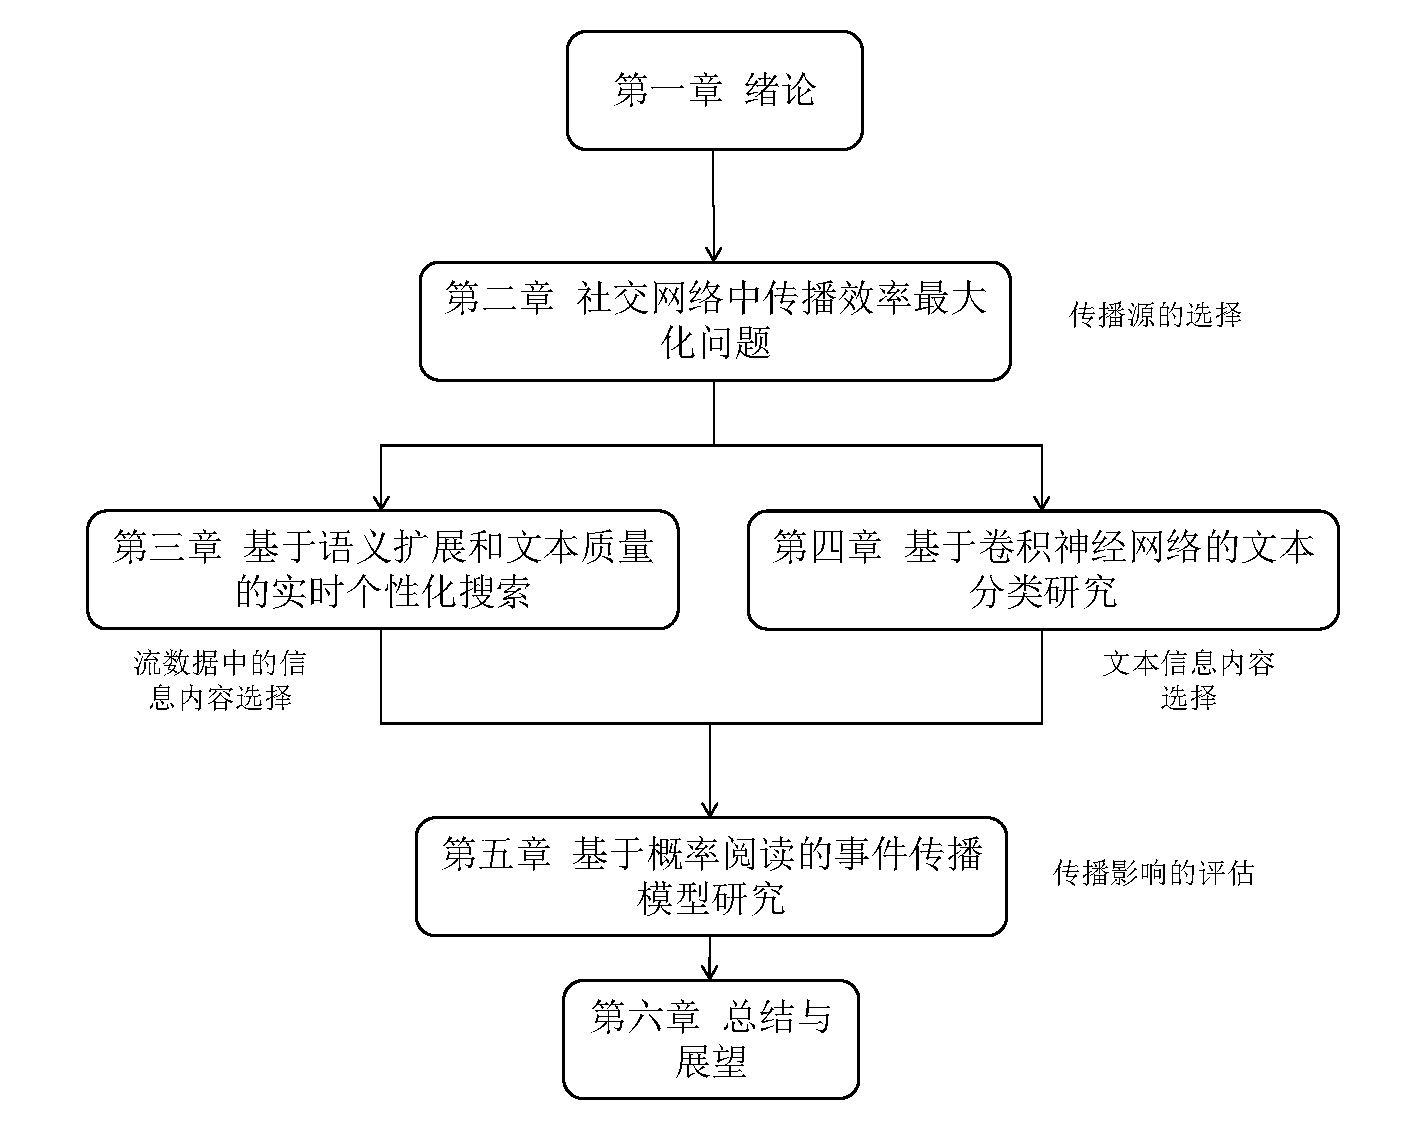
\includegraphics[width=0.8\textwidth]{paperStructure}
    \caption{论文组织结构图}
    \label{fig:paperStructure}
\end{figure}

第一章为绪论,阐述了本文的研究背景与与研究意义,同时对已有的相关研究工作进行了详细的总结,并且概括了本文的研究内容以及创新点。

第二、三、四、五章分别对社交网络信息传播的不同问题进行了研究。第二章研究在社交网络中如何选择传播源的问题,基于传统的影响力最大化问题,考虑传播时延,提出了传播效率最大化问题。第三、四章分别在不同的场景下研究如何选择传播内容的问题。第三章面向社交网络中的流数据,结合语义扩展以及质量模型提出了实时个性化搜索的框架。第四章面向社交网络中的文本数据,应用深度学习技术,提出了一种基于卷积神经网络的文本分类算法。第五章研究社交网络中信息传播的量化问题,以事件为粒度,结合多源信息网络融合、垃圾用户去重以及概率阅读模型,提出了一种新的传播模型用于衡量事件的传播范围。

第六章对本文的工作进行了总结,并对本领域的下一步研究进行了展望。
\chapter{基于语义扩展和文本质量的实时个性化搜索}
\label{2chap:main}
随着社交网络中信息爆炸式的增长,用户越来越难以从海量的信息中获取到自身所需的信息,用户所需的信息往往淹没在其中,这种现象可称之为\textbf{信息洪流}(\textit{information flood})现象。在社交网络、电子商务网站、即时通信等应用中,信息产生的速率以及数量都是过去无法比拟的,如在推特(Twitter)、脸书(Facebook)、新浪微博等社交媒体中,每天都会产生海量的文本信息。根据用户输入的查询,在海量的信息流中实时地检索出高质量的、相关的信息是一个极具挑战性的问题。社交网络中的信息流实时个性化搜索相对于传统的信息检索提出了以下挑战:(1)社交网络中充斥着各种各样话题的信息,而且信息大多数都是以短文本表示,相对于传统的新闻等长文本信息,难以进行语义理解;(2)社交网络中的信息质量参差不齐,难以从中遴选出高质量的信息;(3)社交网络中的信息产生速率快,如何能够实时地检索出用户所需要的信息,将其推送给用户也是一大难点。因此,由于社交网络中数据的信息海量性、主题多样性、数据稀疏性以及社交互动性等特性,传统的个性化检索方法不足以解决社交网络中的信息实时个性化搜索问题。本章针对以上的问题,提出了一个面向推特信息流的实时个性化搜索框架来实现用户的信息实时推荐。本章针对社交网络中信息的特性,提出了一种基于语义扩展和文本质量的实时个性化搜索算法,并在TREC 2015 Microblog Track\upcite{lin2015overview} 测评中验证了算法的性能。首先,我们构造了一个逻辑规则过滤器来选择核心关键词,提高检索的准确率。其次,我们对文本质量进行建模,利用的标注的数据进行训练,以此来对文本的质量的进行打分。训练好的文本质量模型提高了检索的排序性能。然后,我们使用外部语料库来实现语义扩展,例如搜索引擎,知识库等。语义扩展能够使得我们更好地理解用户的偏好和兴趣。最后,我们采用了一个动态的推送策略来自动地推送高质量且相关的信息给特定的用户,这能够避免信息过载。本章中的算法结合了社交网络文本的语义特征和社交属性,针对不同的用户搜索,做了综合性地排序。我们使用TREC 2015 Microblog Track中的真实数据流进行了实验,实验结果显示了本章提出的算法在不同测评指标下,与其他算法相比的优越性。

本章的内容组织如下:第\ref{2sec:motivation} 节介绍了研究动机,讨论了在社交网络环境下进行实时个性化搜索的必要性。第\ref{2sec:definition}节介绍了相关定义,对本章中涉及的相关概念和知识进行了符号化的定义。第\ref{2sec:method} 节介绍了方法描述,详细地阐述了本章提出的系统框架和算法。第\ref{2sec:experiment}节进行了实验分析,验证了本章提出的方法,并且分析了实验结果。最后,第\ref{2sec:conclusion}对本章的内容进行了总结。

\section{研究动机}
\label{2sec:motivation}
随着大数据时代的到来,诸如推特(Twitter)、脸书(Facebook)、新浪微博等的社交网络平台逐渐取代传统的媒体平台,成为新时代的实时信息交互平台。以推特平外为例,据统计,每天平均约有58,000,000条推文(tweet)发布,每天平均处理约2,100,000,000次搜索查询,每月约有115,000,000个活跃的用户\footnote{\url{http://www.statisticbrain.com/twitter-statistics/}}。 在大数据时代,人人都可以是信息的生产者、传播者和接收者,这在一定程度上加速了信息的传播速率。然而,如此庞大的数据量使得用户在社交网络平台中搜索查询时面临了信息过载的问题,用户很难检索到自己需要的信息,亦或用户所需的信息淹没在了众多的信息之中。尤其是社交网络平台中的信息内容囊括了众多领域,其中的话题种类繁多,这使得用户难以搜索到相关性强而且高质量的文本信息。在社交网络平台中,传统的信息检索方法变得耗时长而且信息检索方式难以适用。因此,在大数据时代,为了满足用户实时获取相关信息的需求,需要一种面向社交网络的新的信息检索方法。

在传统的信息检索流程中,往往是用户根据自己所需,输入关键字进行查询,系统根据用户的查询,搜索到相关的结果,并进行排序,返回给用户。而在社交网络平台中,信息产生速率快,信息以数据流的形式给出,同时用户希望系统能够自动地推送相关的信息,而不是用户通过查询来获取信息。因此,在社交网络中的信息实时个性化搜索的流程与传统的信息检索流程不尽相同。在社交网络中,信息的实时个性化搜索流程一般是用户将查询搜索以关键词的形式给出,然后系统根据用户的查询在信息流中实时地处理文本信息,将相关的信息自动地推送给用户。

由美国国家标准与技术研究院(NIST)主办的文本检索会议(TREC)是由多个测评项目组成的一个致力于解决新时代信息检索问题的测评大会,涉及智能问答、医疗诊断、实体识别、信息推荐等领域。TREC自2011年起设立了微博实时推荐(Microblog Track)\upcite{ounis2011overview,soboroff2012overview,lin2013overview,lin2014overview,lin2015overview} 这一个子任务,目标是解决在社交网络中信息的实时个性化搜索问题。从设立后,TREC Microblog Track便吸引了全世界的参赛者参加,与智能实时问答(TREC LiveQA Track)成为了TREC中最火热的两个子任务。Microblog Track 的任务是针对不同用户,智能地分析用户的兴趣爱好,自动地、实时地为用户推送相关的、高质量的信息,涉及到众多科学领域,包括机器学习、自然语言处理、信息检索、人工智能等。如图\ref{fig:twitter_search}所示,在社交网络平台中,用户是信息的生产者,用户将源源不断地发布信息,其中包括有趣的信息和一些无用的信息。同时,用户又是信息的接收者,用户通过定制自身感兴趣的话题和内容,系统智能地分析其兴趣爱好,针对不同的用户,在推特信息流中自动地、实时地为用户推荐相关的、高质量的信息。例如将饮食信息推荐给美食家、将财经信息推送给金融家、将商旅信息推送给旅行者等,同时将一些低质量无意义或者无人关注的信息丢弃。

\begin{figure}[!htbp] % use float package if you want it here
  \centering
  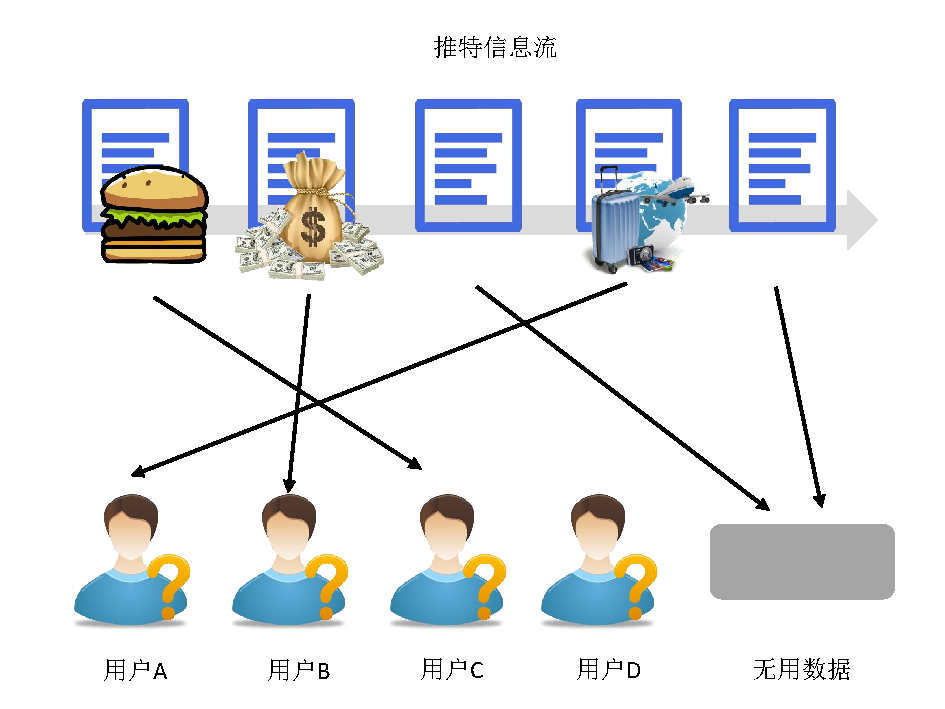
\includegraphics[width=0.8\textwidth]{twitter_search}
  \caption{社交网络平台中信息的实时个性化搜索示意图}
  \label{fig:twitter_search}
\end{figure}

为了解决针对不同用户,为其实时地搜索出相关性强、高质量的信息,许多已有的个性化推荐\upcite{Xie2015Personalized,sontag2012probabilistic,wang2013personalized,tang2015personalized} 以及协同搜索\upcite{liang2014Collaborative,vosecky2014collaborative,xue2009user,yang2014survey} 的工作对这个问题进行了一定的研究。但是很少有面向社交网络个性化搜索的研究,特别是对于实时搜索推荐技术的研究。目前已有的机器学习、自然语言处理、信息检索、人工智能等研究对于社交网络中的实时个性化搜索问题提供了许多帮助。文本分类以及排序的研究\upcite{canuto2015efficient,severyn2015learning,ren2014hierarchical,paik2013novel} 能够为了社交网络中的信息检索提供支持。同时,查询分析以及优化技术\upcite{gao2013query,Letelier2012Static,si2014users} 能够使得信息检索有着显著的提升。

然而,社交网络的环境与传统的新闻、论坛等Web环境有着较大的区别。因此,为了满足社交网络中用户获取信息的需求,这将需要建立新的模型、研究新的方法来解决这一问题。在社交网络中,实现信息的个性化实时推荐面临的主要挑战可以总结如下:
\begin{itemize}
  \item \textbf{信息海量性},在社交网络中,信息产生的速率快,网络中的每一个用户同时扮演着信息生产者、信息传播者和信息接收者的角色。如此高容量的信息流需要一个新的模型来适应持续不断变化的语义特征。
  \item \textbf{主题多样性},社交网络中的信息内容包罗万象,覆盖了许许多多的领域和话题。如果主题模型不能区分众多的话题,这将导致噪声的引入以及不准确的话题模型以及用户模型。
  \item \textbf{数据稀疏性},在社交网络中,信息在不同的主题上的分布是不均匀的,在某些主题上信息量大,而在某些主题上信息是稀疏的。有效的主题模型需要解决数据稀疏性所带来了的影响。
  \item \textbf{社交互动性},社交网络中的用户之间有着丰富的互动信息,与传统的文本信息不同,社交网络中的信息包含了许多有价值的结构化的社交属性。适当地利用这些社交属性能够提高搜索的性能,但是这需要对这些社交属性进行相关性的选择。
\end{itemize}

为了解决上述面临的挑战,本章提出了一种基于语义扩展和文本质量的实时个性化搜索框架,该框架综合考虑了用户的偏好、语义特征和社交属性。首先,本章基于语义扩展提出了一种布尔逻辑关键词过滤(Boolean Logic Keyword Filter)的用户模型。该模型依靠外部搜索引擎提供的知识进行建立,建立的用户模型充分利用了查询扩展以及检索结果的重排序来提高推荐结果的相关性。最终的实验评估证明该模型显著地提高了检索的召回率。此外,本章还基于逻辑回归提出了一种文本质量模型,该模型利用推文的社交属性来评估其文本的质量。该模型能够对推文的文本内容,是否受到大众的认可等进行评估,因此它能帮助系统返回高质量的推文。最终的实验评估证明该模型显著地提高了检索结果的排序性能。

\section{相关定义}
\label{2sec:definition}
本节首先将对社交网络中的实时个性化搜索的任务进行定义,并将其形式化,然后对TREC 2015 Microblog Track的具体任务进行描述。

社交网络中的实时个性化搜索任务可以描述如下。在社交网络中平台中,令信息流表示为\textbf{T},信息流在社交网络中随着时间不断地产生,信息流\textbf{T}中包含许多种类的话题。令\textbf{P}表示用户集合,每一个用户$p_i \in \textbf{P}$表示着用户感兴趣的一个话题,用户的兴趣爱好可以通过文本等形式来表示。则社交网络中的实时个性化搜索任务可以定义如下,
\begin{mydef}[实时个性化搜索]\label{def:realPrnzdSearch}
在社交网络中,给定信息流\textbf{T}以及用户集合\textbf{P},实时个性化搜索的目的是针对不同的用户兴趣爱好$p_i \in \textbf{P}$,自动地实时地为其推荐高质量的、相关的信息。
\end{mydef}

根据定义\ref{def:realPrnzdSearch}可知,社交网络中的实时个性化搜索需要解决的几个核心关键问题如下。首先是如何表示信息流与用户,其次是如何实现实时推荐,以及如何保证信息的高质量和高相关性。社交网络平台中信息的实时个性化搜索任务可以通过图\ref{fig:real-timeSearch}来表示。
\begin{figure}[!htbp] % use float package if you want it here
  \centering
  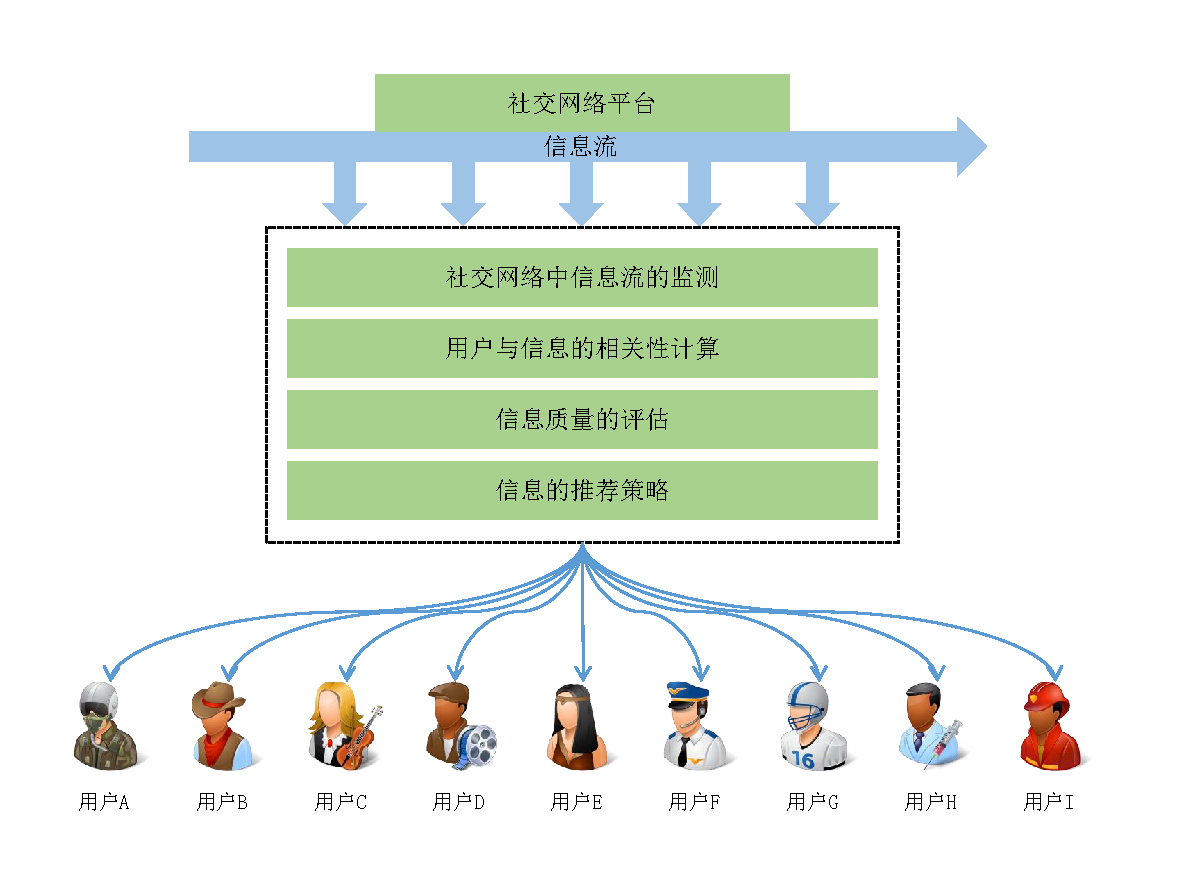
\includegraphics[width=\textwidth]{real-timeSearch}
  \caption{社交网络平台中信息的实时个性化搜索任务图}
  \label{fig:real-timeSearch}
\end{figure}

任务首先要求系统能够实时地监测社交网络中的信息流,然后对不同的用户建立兴趣模型,分析信息与用户之间的相关性。同时任务还要求系统能够对信息的质量做出评估,包括真实性、内容丰富性等。最后,系统需要采取一个良好的推送策略,使得用户不至于淹没在信息中。

TREC 2015 Microblog Track的任务目标是\textbf{实时信息流过滤},实质上也是实时个性化搜索的一种形式。在Microblog Track中,实时信息流过滤的任务目标是根据不同用户的兴趣模型来监测社交媒体中的信息流。值得注意的是,上述的兴趣模型的概念是不同于传统的临时查询。该场景中,交互流程不是用户输入一次查询,然后系统返回结果给用户。该场景不存在实际的查询,取而代之的是系统根据用户的兴趣模型主动地推送\textbf{有趣的}信息给用户。

什么样的信息是有趣的可以考虑如下两个实际的任务模型来帮助更好地理解。
\begin{itemize}
  \item \textbf{场景A:即时性信息推送},在场景A中,用户是定位在使用移动设备的场景,用户可以即时地查看消息。系统基于用户的兴趣模型来判别消息之于用户是否是有趣的,被系统判别为有趣的信息将实时地推送到用户的移动设备(例如手机、平板等)。场景A中的任务目的是上述的推送需要在消息产生的相对较短的时间内完成,该场景中的信息假设是相对较短的。
  \item \textbf{场景B:周期性邮件摘要},在场景B中,用户是定位在使用固定设备的场景,用户周期性的查看消息。与场景A相同,统基于用户的兴趣模型来判别消息之于用户是否是有趣的。但是被系统判别为有趣的信息将被聚集成一个邮件摘要,并且周期性的推送给用户。该场景中的每一个单一信息假设是相对较短的,聚集成的邮件摘要可能很长,我们可以认为这是\textbf{个性化头条新闻}。
\end{itemize}

两个场景都假设推送给用户的消息相对较短,是短消息。因此,推送的消息是否有趣可以根据用户阅读消息的长度或者条数来进行衡量。可以看出,TREC 2015 Microblog Track的任务目标是在两种不同的场景中来考虑社交网络平台中信息的实时个性化搜索问题。

任务中的推特信息流一条推文以JSON格式保存,字段信息如表\ref{2tab:tweetJSON}所示。
\begin{table}[!htbp]
\centering
\caption{推文JSON数据的部分字段信息}
\begin{tabular}{|p{4cm}|p{7cm}|}
\hline
\textbf{字段} & \textbf{描述} \\
\hline
$created\_at$ & 推文的创建时间\\
\hline
$id$ & 推文的ID\\
\hline
$text$ & 推文的文本信息\\
\hline
$source$ & 推文的发布终端\\
\hline
$in\_reply\_to\_status\_id$ & 回复的推文的ID\\
\hline
$user$ & 发布推文的用户信息\\
\hline
\end{tabular}
\label{2tab:tweetJSON}
\end{table}

表\ref{2tab:tweetJSON}中$created\_at$是推文创建的时间,即发布时间。$id$是推文的ID,是唯一的。$text$是推文的文本信息,为短文本,不超过140个字符,可能存在超链接。$source$是推文的发布平台,例如推特Web端,推特手机端,或者通过其他的平台转发至推特等。$in\_reply\_to\_status\_id$是指该推文是否为转发回复其他的推文,如果不是则字段为$null$,如果是则为转发的推文的ID。$user$是指发布推文的用户,也是一个JSON格式的数据,其字段内容在表\ref{2tab:userJSON}中给出。
\begin{table}[!htbp]
\centering
\caption{用户JSON数据的部分字段信息}
\begin{tabular}{|p{4cm}|p{7cm}|}
\hline
\textbf{字段} & \textbf{描述} \\
\hline
$created\_at$ & 用户的创建时间\\
\hline
$id$ & 用户的ID\\
\hline
$screen\_name$ & 用户的名称\\
\hline
$location$ & 用户的地理信息\\
\hline
$description$ & 用户的自我描述\\
\hline
$followers\_count$ & 用户的粉丝数\\
\hline
$friends\_count$ & 用户的好友数\\
\hline
$favourites\_count$ & 用户收藏推文的数目\\
\hline
$statuses\_count$ & 用户发布推文的数目\\
\hline
$utc\_offset$ & 用户所在时区\\
\hline
$profile\_image\_url$ & 用户的头像\\
\hline
$lang$ & 用户的语种\\
\hline
\end{tabular}
\label{2tab:userJSON}
\end{table}

表\ref{2tab:userJSON}中$created\_at$为用户账号建立的时间。$id$为用户的ID,是唯一的。$screen\_name$为用户的名字。$location$为用户的地理位置,由用户自己填写。$description$为用户对自己的描述,为一段文本信息。$followers\_count$为用户的粉丝数,即关注该用户的用户数。$friends\_count$为用户的好友数,即用户关注的用户数目。$favourites\_count$为用户收藏的推文的数目。$statuses\_count$为用户历史上发布推文的数目。$utc\_offset$为用户所在的时区的偏差值,单位为秒。$profile\_image\_url$为用户的头像,如果用户没有自定义头像,则为系统默认头像。$lang$为用户的常用语言。
%在实时信息流过滤任务中,信息即为推文。在测评阶段,进行测评的系统将监测推特的实时样本信息流并根据用户的兴趣模型(相当于特定的话题)来识别有趣的信息。为了描述的简洁性,我们将上述过程称之为\textbf{兴趣用户的追踪}。

\section{方法描述}
\label{2sec:method}
在本节中,我们设计了一个面向社交网络的实时信息流推荐的系统框架。首先,与传统的信息检索系统相似,信息以及用户的语义特征被提取出来,数据的预处理用于过滤掉此阶段中无用的信息。其次,为了计算信息与用户之间的相似度(即相关性),基于外部语料库训练得到的词向量模型来表述提取的特征。除此之外,系统将文本的质量也考虑在内。高质量的文本往往包含高质量的信息,本节提出了一个基于逻辑回归模型的文本质量评估算法来对文本的质量进行衡量。然后,基于得出的相关性与质量,系统针对不同的用户对信息进行评估。一条相关的、有意思的信息将被归类到最相关的类别中,即归类到最相关的用户。最后,为了避免信息洪流、保持消息推送的实时性,本节提出了一个动态的推送策略。因此,用户将实时地收到相关性强、质量高的信息,并且能够避免淹没在信息中。

\subsection{系统框架}
\label{2subsec:systemOverview}
目前在社交网络中,用户只能接收到其关注用户的信息推送,而且这些信息只是简单的按照时间进行排序。理想的搜索系统应当能够分析用户的兴趣爱好,并且自动地推送相关的、高质量的信息给用户。为了满足这一需求,一个面向推特的实时个性化搜索系统的框架设计如图\ref{fig:systemFramework}所示。
\begin{figure}[!htbp] % use float package if you want it here
  \centering
  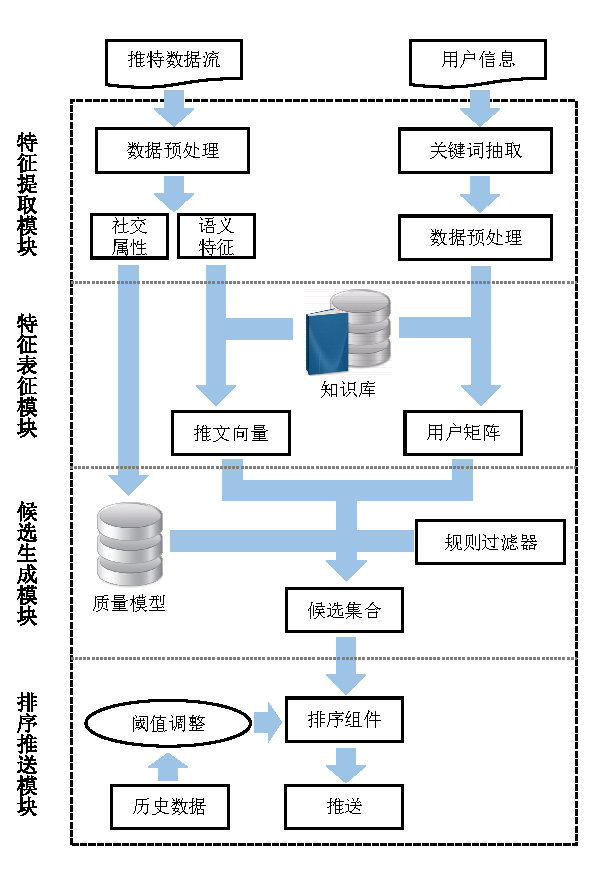
\includegraphics[width=0.7\textwidth]{systemFramework}
  \caption{实时个性化搜索系统框架图}
  \label{fig:systemFramework}
\end{figure}

如图所示,系统主要包括四个主要的模块,分别如下所示。
\begin{itemize}
  \item \textbf{特征提取模块},该模块监测推特信息流,并且接收用户的搜索请求。值得注意的是,在实时个性化搜索任务中,用户的搜索请求相当于某个话题内容的订阅。用户事先输入搜索后,在相关的信息发布时实时推送给用户。推特信息流通过TREC-API\footnote{\url{https://github.com/lintool/twitter-tools}}工具监测。用户的搜索由官方提供,以$p_i \in \textbf{P}$表示。在特征提取之前,数据的预处理将用来过滤掉无用的信息。对于推特信息流,系统提取其语义特征以及社交属性;对于用户信息,系统提取搜索中的关键词作为基础特征。
  \item \textbf{特征表征模块},该模块通过几种技术来扩展及表征所提取的语义特征。推文信息以及用户信息通过该模块进行了语义增强,该模块使得推文以及用户之间的相关度计算更加的方便。
  \item \textbf{候选生成模块},该模块通过语义特征以及社交属性将推文分类到与之最相关的用户。这一过程同时考虑了相关性以及推文的质量,因此用户收到的信息不仅是有趣的而且是高质量的。
  \item \textbf{排序推送模块},该模块通过最终的得分来对每个用户的推文候选队列进行排序,并且利用历史数据进行阈值的动态调整。该模块能够保证用户不错过重要的高质量的信息,又不至于淹没在过多的信息中。
\end{itemize}

在之后的小节中,我们将详细地介绍每一个模块应用的算法以及实现。

\subsection{特征提取模块}
\label{feaureExtraction}
推文信息依靠监测推特的抽样信息流来获取\upcite{wang2015assessor}。在获取到推文后,数据的实时预处理用来过滤掉此阶段内无效的信息,减少无意义的以及冗余的信息。推特数据流上的相关数据预处理方法包含如下一些技术,
\begin{itemize}
  \item \textbf{语言识别},根据任务要求,非英文的推文将被直接过滤掉来简化问题的复杂度。本系统中使用的工具为\textbf{无限元模型语言识别}(\textit{Language Detection with Infinity Gram}),简称为ldig\footnote{\url{https://github.com/shuyo/ldig}}。ldig工具是一个针对短文本消息(例如推特)的语言识别器,能够支持对于17种语言的识别,准确率达到了99.1\%。除此之外,系统还使用了基于字符编码集的语言识别方法来区分英文句子和非英文句子。通过训练得出一个阈值,包含英文字符多的推文将被保留,其余的将被过滤掉。
  \item \textbf{冗余过滤},社交网络中由于复制,转发等行为使得相同信息的推文存在着很多的冗余,如果不进行冗余过滤,那么将会有很多相同的内容推送给用户,使得用户淹没在重复的信息中。因此,对于内容相同或者相似的推文,系统只保存一个副本。为了实现该目标,一种方法是利用表\ref{2tab:tweetJSON}中提到的推文$id$字段和$in\_reply\_to\_status\_id$字段来识别冗余信息。如果推文是原创信息,则我们记录其$id$值;如果推文是转发信息,则可以检查该推文转发推文的$id$是否已经存在来判别是否是冗余信息。每当一条新的推文被爬取时,首先来检查推文的$id$来做冗余消除。该方法简单有效,能够迅速滤除掉大部分的冗余信息。但是当推文是复制其他推文的信息或者做出微小的改动,则该方法无法识别。因此,另外一种冗余消除技术,$simhash$技术被应用。$simhash$技术是用于处理网页冗余的技术,该方法将一个文档转换成一个数字指纹(即一串定长的0-1编码),被称为\textbf{哈希相似码}。两个文档的哈希相似码之间的汉明距离(\textit{hamming distance})越短,则说明两个文档之间的相似度越大。哈希相似码的计算公式如下所示,
  \begin{equation}
  \label{simhash}
    {\mathbf{s}_{hash}} = sign(\sum\nolimits_{i = 1}^n {{w_i} \cdot {\mathbf{c}_i}} )
  \end{equation}
其中$\mathbf{c}_i$是第$i$个词的哈希码,为一个定长的向量,$w_i$是该词的权重,为标量,$sign$是是一个符号函数,让结果向量中的每一个比特的正数位变成1,负数位变成0。simhash算法的过程大概如下。首先,对文档进行关键词抽取,得到特征$\mathbf{c}_i$和权重$w_i$。然后,对所有特征进行加权的位计算。最后,对得到的结果进行哈希码的生成,这个产生值和具体采用的算法有关,这里采用的一个简单的符号函数。将推文转换成哈希相似码后,我们就可以利用推文之间的汉明距离来判别推文间的相似性,来进行冗余消除。基于推文的$id$进行冗余消除是一种高效的方法,能够解决大多数情况下的问题,但是对于复制或者修改的内容无法识别。simhash算法是基于推文的内容进行冗余消除,能够有效地解决内容相似的推文冗余,但是相比于基于推文$id$的方法耗时会长一些,因为计算哈希相似码的过程将会有额外的计算量。在本章提出的系统中,两种算法被结合起来完成冗余消除。首先利用基于推文$id$的方法进行粗的冗余消除,如果无法判别则计算推文的哈希相似码后,根据汉明距离进行判别。
\end{itemize}

在数据的预处理后,我们将推文信息和用户信息的语义特征和社交属性抽取出来。对于推文,名词以及动词是句子中最重要的部分。因此,退文中的名词以及动词(除去停用词)被抽取出来作为语义特征,并且每一个词都根据其在句子中的重要性得到一个不同的权重。一条推文的语义特征可以表示成$\mathbf{ts} = \{ {w_1}{t_1},{w_2}{t_2},\cdots,{w_n}{t_n}\}$,其中$\mathbf{ts}$表示一条推文,$t_i$表示一个词语,$w_i$为该词语的权重。词语的权重与该词语在句子中的位置、出现的频率等有关。



\section{实验分析}
\label{2sec:experiment}

\section{本章小结}
\label{2sec:conclusion}



\chapter{社交网络中传播效率最大化}
\label{3chap:main}
\textbf{影响力最大化}(\textit{Influence Maximization})在许多的社交网络应用中扮演着举足轻重的角色,例如市场营销、商业活动以及竞选活动等等。研究信息传播模型以及机理的一个典型目的便是市场营销。在现实社会中,人或者事物都是通过某种关系来连接,形成了一个巨大的网络。因此,信息传播可以选择一小部分节点激活做为种子节点集合,然后通过信息的传递,在整个网络中产生一个大范围的影响。从技术方面来说,影响力最大化问题是在给定网络和传播模型的条件下,研究如何选择种子节点集合使得传播的影响范围最大化。影响力最大化问题由于其的问题真实、应用性广的特点,吸引了许许多多的研究,包括信息传播模型的研究和计算影响力最大化的方法。但是,仍然有着一些需求在实际应用中得不到满足。

在信息传播过程中,一个被激活的节点将会尝试在下一个时刻激活它的邻居节点。所以,除去种子节点外,每一个被激活的节点在被激活之前都会有一个时间延迟,我们称之为\textbf{传播时延}(\textit{propagation time delay})。如果一个节点在信息传播结束时,仍然未被激活,则该节点的传播时延可以看作无穷大。在传统的影响力最大化问题中,传播时延没有被考虑在内,而研究整个网络的传播时延是非常有意义的,它可以度量选择的种子节点集合的传播效率。出于这种需求,本章提出了一个新的问题,传播效率最大化问题。该问题将传播时延考虑在内,在给定网络和传播模型的条件下,研究如何选择种子节点集合使得传播效率最大化。传播效率最大化问题与影响力最大化问题虽然相似,但是两个问题的侧重点不尽相同。传统的影响力最大化问题研究的是如何使得传播的范围最广,不考虑节点的传播时延。而本章提出的传播效率最大化问题将传播时延考虑在内,研究如何使得传播效率最大化。

本章主要的工作可以总结如下。首先,基于传统的影响力最大化问题,我们将传播时延考虑在内了来探究传播效率,提出了传播效率最大化问题,研究给定网络和传播模型的条件下,研究如何选择种子节点集合使得传播效率最大化。其次,本章证明了传播效率最大化问题是一个NP-hard问题,而且在独立级联模型下计算传播效率的过程是一个\#P-hard的问题。然后,我们证明了传播效率函数在独立级联模型下是\textbf{子模}(\textit{submodular})的。最后本章设计了三个算法来解决提出的传播效率最大化问题,并且在真实数据集上验证了这些算法。实验结果展示了所提出的算法的性能。

本章的内容组织如下:第\ref{3sec:motivation}节介绍了研究动机,讨论了传统的影响力最大化问题的不足和考虑了传播时延的传播效率最大化问题的意义。第\ref{3sec:definition}节介绍了相关定义,对本章中相关概念和所提出的问题进行了符号化的定义。第\ref{3sec:method}介绍了方法描述,详细地阐述了本章解决问题的方法以及相关证明过程。第\ref{3sec:experiment}节进行了实验分析,设计了一系列的实验,验证了本章所提出的方法,并对实验结果进行了分析。最后,第\ref{3sec:conclusion}对本章的内容进行了总结。

\section{研究动机}
\label{3sec:motivation}
随着社交网络的兴盛发展,信息传播的速率变得越来越快。在传统的媒体环境下,一条消息需要通过较长时间才能传播到一定的范围。在社交网络中,个人通过关系(例如关注、好友等)连接形成网络,信息在网络中通过转发、复制等行为进行传播,信息传播的速率极大的加快了。在传统的媒体环境下,个人都是通过单一信息源(例如新闻、论坛等)来接收信息,接收信息的渠道受限,信息在个体之间难以形成传播扩散。而在社交网络环境下,个人既可以是信息的接收者也可以是信息的发布者,个人可以接收到在网络中与之相连的个人推送的信息。与此同时,信息通过个人构成的网络进行传播。影响力最大化问题是信息传播中的一个典型问题,是在给定网络和传播模型的条件下,研究如何选择种子节点集合使得传播的影响范围最大化。
\begin{figure}[!ht]
    \centering
    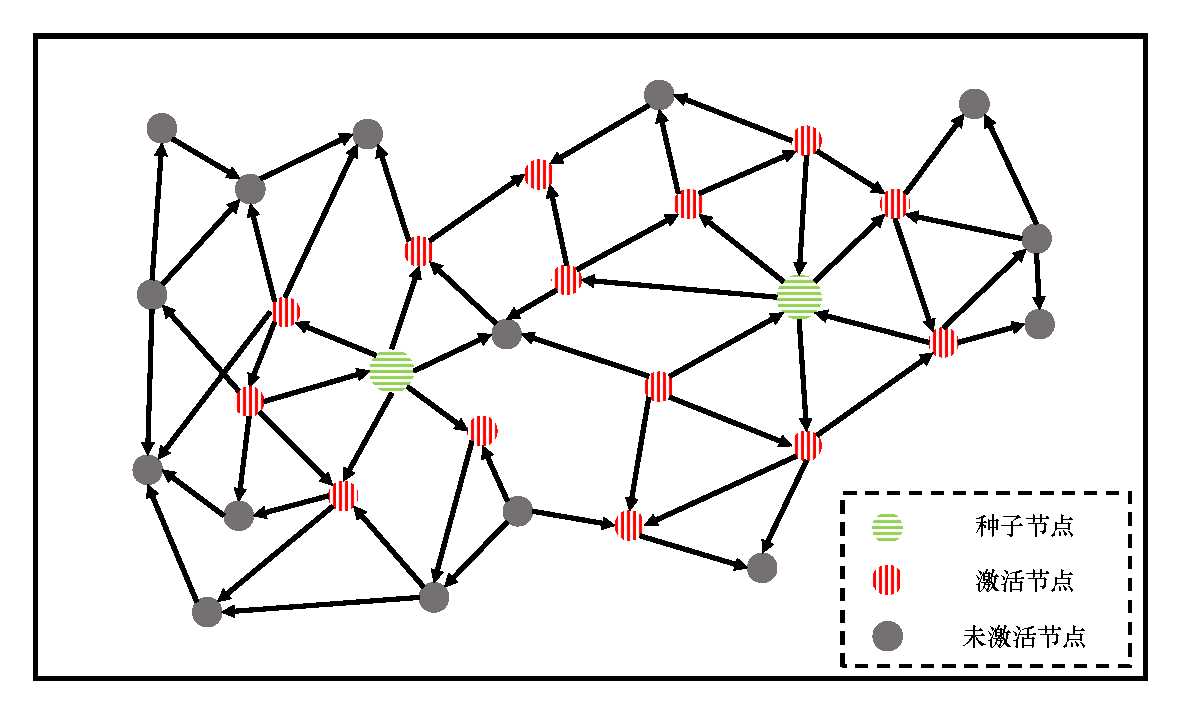
\includegraphics[width=0.8\textwidth]{figures/infoDiffExp.pdf}
    \caption{信息传播以及影响力最大化示意图}
    \label{fig:infoDiffExp}
\end{figure}

图\ref{fig:infoDiffExp}为一个信息传播以及影响力最大化示意图,其中的点代表着个体,边代表着社交关系。图中所示的例子为选中了绿色节点为种子节点,进行信息传播后最终产生的传播范围。红色的节点代表接受了信息,灰色的节点代表未接受信息。影响力最大化的问题即是研究如何选取初始的种子节点集合,使得传播范围最大化。

市场营销是研究信息传播模型以及机理的一个典型驱动。市场营销的过程可以简述如下,一个公司希望在社交网络中通过“口碑效应”推动一款新产品或者一种新理念。一种有成本效益的方法是寻找到整个网络中有影响力的个人,然后投入资源来使他们接受这款产品,例如赠送样品、免费试用、优惠折扣等。这样的举措是希望这些有影响力的个人在接受新产品或者新理念后,能够驱使社交网络中的其他个人也来接受新产品或者新理念,然后在社交网络中产生一个大的级联效应,从而使得更多的个体接受新产品或者新理念。为了达到市场营销这一目的,我们需要对两个重要的问题进行研究:(1)如何对网络中的信息传播过程进行建模,包括模型参数的学习等;(2)如何在给定的传播模型的条件下,设计一个有效的方法来寻找能够最大化影响力的节点集合。本章着重对第二个问题进行研究。

影响力最大化问题作为市场营销的一种算法技术首先被Domingos和Richardson\upcite{domingos2001mining}所提出,该问题基于马尔科夫随机场的概率框架。而后,Kempe等人\upcite{kempe2003maximizing}首次将影响力最大化问题形式化成为一个离散的随机优化问题。信息传播的过程可以简述如下,在一个给定的网络中,选择部分节点做为种子集合,这些种子节点将会按照一定的规则去激活它们的邻居节点。被激活的节点在下一时刻将拥有能力去激活它们的邻居节点,这个过程将一直持续到没有新的节点可以被激活,整个信息传播的过程才会停止。影响力最大化问题是在给定网络和传播模型的条件下,研究如何选择种子节点集合使得传播的影响范围最大化,即激活的节点数目最大化。从上述信息传播过程的描述中,我们可以得知,一个被激活的节点会在被激活的下一时刻尝试激活它的邻居节点。因此,除去种子节点外,网络中的节点在被激活前都会有一个时间延迟,我们称之为传播时延。如果一个节点在信息传播结束时,仍然未被激活,则该节点的传播时延可以看作无穷大。而影响力最大化问题仅仅考虑了传播范围,忽略了节点的传播时延。在真实的场景中,例如市场营销、商业活动、竞选活动等,传播时延在信息传播中是一个非常重要的因素。为了让其他人接受自己的新产品或者新理念,人们总是希望能够尽快地将消息传播到群体中。我们以\textbf{传播效率}(\textit{influence efficiency})来表示传播时延的倒数,传播时延小,则传播效率大。如果节点在信息传播结束时仍然未被激活,那么该节点的传播效率则为0。以上是针对单个节点的传播时延和传播效率的分析,下面我们对整个网络的传播时延和传播效率进行分析。在给定一个传播网络和初始的种子节点集合的情况下,如果整个网络中所有节点的传播效率高,这就意味着在信息传播过程中,网络中的节点将被迅速地激活。我们设想如下,针对传统的影响力最大化问题有两种选择种子节点集合的策略,它们有着相同的传播范围,即能够在信息传播过程结束时能够激活相同的节点数目。但是,这两种策略中,网络中的传播时延可能是不同的,即不同策略在同一网络中的传播效率是不同的,而这一问题在传统的影响力最大化问题中是没有讨论的。

\section{相关定义}
\label{3sec:definition}
在本节中,第\ref{3subsec:model}节首先对\textbf{独立级联模型}(\textit{Independent Cascade Model})以及在独立级联模型下的影响力最大化问题进行回顾,然后介绍了几种解决影响力最大化问题的方法,并且对这些算法进行分析,包括影响力函数期望的单调性和子模性等。其次,第\ref{3subsec:efficiency}节提出了\textbf{传播效率最大化}(\textit{Influence Efficiency Maximization})问题,该问题是基于传统的影响力最大化问题,将传播时延考虑在内,研究如何使得整个网络的传播效率最大化。同时,第\ref{3subsec:efficiency}节对传播效率最大化问题进行了形式化的描述,分析了传播效率最大化和影响力最大化问题的区别。

为了便于参照,表\ref{3tab:notation}中列出了频繁使用的符号。

\begin{table}[ht]
\centering
\caption{常用符号列表}
\begin{tabular}{|p{2cm}|p{10cm}|}
\hline
\textbf{符号} & \textbf{描述} \\
\hline
$\mathcal{G}=\left(\mathcal{V},\mathcal{E}\right)$ & $\mathcal{G}$是社交网络构成的图,$\mathcal{V}$是节点集合,$\mathcal{E}$是边的集合\\
\hline
$\mathcal{H}=\left(\mathcal{V},\mathcal{Z}\right)$ & $\mathcal{H}$是基于图$\mathcal{G}$生成的超图(参见\ref{alg:res}),$\mathcal{V}$是节点集合,$\mathcal{Z}$是超边集合\\
\hline
$n$ & $\mathcal{G}$或者$\mathcal{H}$的节点的数目 \\
\hline
$m$ & $\mathcal{G}$的边的数目 \\
\hline
$k$ & 种子节点集合的大小 \\
\hline
$p^\mathcal{G}_{u,v}$ & 节点$u$激活节点$v$的概率 \\
\hline
$I\left(S\right)$ & 种子节点集合$S$的影响力 \\
\hline
$RR\left(v\right)$ & 节点$v$的反向可达集合 (参见定义\ref{def:rrSet}) \\
\hline
$e_{u,v}$ & 节点$u$到节点$v$的传播效率(参见方程(\ref{eq:efficiency})) \\
\hline
$T\left(S\right)$ & 种子节点集合$S$在图$\mathcal{G}$中的传播效率(参见方程(\ref{eq:influenceEfficiency}))\\
\hline
$T'\left(S\right)$ & 种子节点集合$S$在超图$\mathcal{H}$中的传播效率(参见算法\ref{alg:res})\\
\hline
\end{tabular}
\label{3tab:notation}
\end{table}

\subsection{传播模型以及影响力最大化问题}
\label{3subsec:model}
本章采用一种广泛采用的信息传播模型,独立级联模型,进行传播影响的研究。在该模型下,一个社交网络可被建模表示为一个有向图$\mathcal{G}=\left(\mathcal{V},\mathcal{E}\right)$,其中$\mathcal{V}$代表网络中的个体,$\mathcal{E}$表示个体之间的社会关系。此外,图中的每一条边$\left(u, v\right) \in \mathcal{E}$上都关联着一个传播概率$p^\mathcal{G}_{u,v}$,表示着节点$u$到节点$v$的影响力度。如果传播概率$p^\mathcal{G}_{u,v}$越大,则节点$u$更加可能激活节点$v$。如果图$\mathcal{G}$与上下文无关,本章则用$p_{u,v}$来表示节点$u$到节点$v$的传播概率。

独立级联模型描述了一个直观的信息传播过程,其过程如下。在独立级联模型下,网络中的个体会被其邻居所影响,这些影响之间是独立的。给定一个种子节点集合$S \subseteq \mathcal{V}$,信息传播在独立级联模型下是如下运作的。定义$S_t$为在$t \geq 0$的时刻激活的节点集合。显然,在$t=0$时刻时,满足$S_0=S$。在$t+1$时刻,每一个在$t$时刻被激活的节点$u \in S_t$会独立地去尝试激活它的出度边指向的未被激活的邻居节点$v \in \mathcal{V} \setminus \cup_{0 \leq i \leq t}S_i$,激活节点$v$的概率等于$p_{u,v}$。当节点$u$尝试了去激活所有它的出度边指向的节点后,它在信息传播的之后过程中将不再会有机会去激活。即在$t$时刻被激活的节点$u$只会在$t+1$时刻去尝试激活它的出度边指向的邻居节点。当$t$满足$S_t = \emptyset$时,整个信息传播过程停止。

\begin{figure}[ht]
   \begin{minipage}{0.48\textwidth}
     \centering
     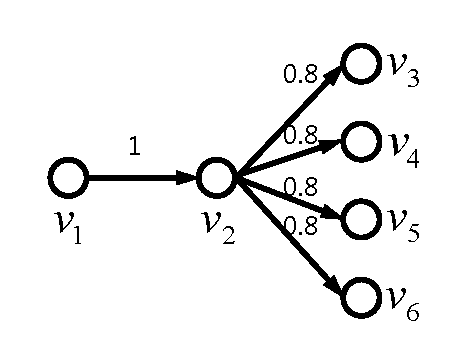
\includegraphics[width=0.8\linewidth]{figures/tinyGraph.pdf}
     \caption{社交网络中的信息传播概率图$\mathcal{G}$}\label{fig:tinyGraph}
   \end{minipage}
   \hfill
   \begin {minipage}{0.48\textwidth}
     \centering
     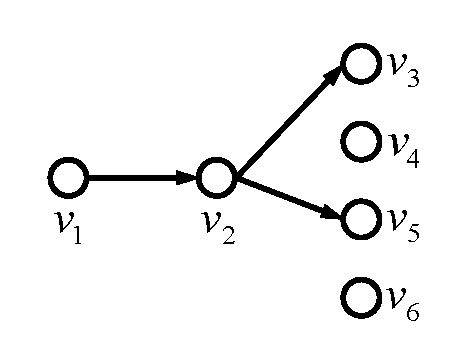
\includegraphics[width=0.8\linewidth]{figures/tinyRandomGraph.pdf}
     \caption{随机实例图$g$}\label{fig:tinyRandomGraph}
   \end{minipage}
\end{figure}

以图\ref{fig:tinyGraph}中的社交网络$\mathcal{G}$为例,考虑种子节点集合$S=\left\{v_1\right\}$的信息传播过程。图\ref{fig:tinyGraph}中边上的数值代表着节点之间的传播概率$p^\mathcal{G}_{u,v}$。整个信息传播的过程可以描述如下。在$t=0$时刻,由于节点$v_1$是种子节点集合中唯一的节点,因此节点$v_1$被激活。在$t=1$时刻,因为节点$v_1$在$t=0$时刻被激活,而且图$\mathcal{G}$中存在一条从$v_1$到$v_2$概率为1的边,节点$v_1$将依概率1去激活节点$v_2$。因此,节点$v_2$将在$t=1$时刻被激活,$S_1=\left\{v_2\right\}$。此后,在$t=2$时刻,节点$v_2$将尝试去激活节点$v_3$、$v_4$、$v_5$以及$v_6$。假设这一次信息传播过程如图\ref{fig:tinyRandomGraph}所示,节点$v_3$和$v_5$被激活,则$S_2=\left\{v_3, v_5\right\}$。然后,在$t=3$时刻,由于被激活的节点没有后继节点可被激活,整个信息传播过程在此时刻停止。定义$I\left(S\right)$为在种子节点集合是$S$的条件下,整个信息传播过程中激活的节点数目,代表信息传播过程中的影响力。在上述的图$\mathcal{G}$的一次信息传播过程中,影响力$I\left(S\right)=4$。

给定一个种子节点集合$S$,定义$\mathbb{E}_\mathcal{G}\left[I\left(S\right)\right]$表示种子节点集合在图$\mathcal{G}$中影响力的期望,它等于以种子节点集合为传播源,在图$\mathcal{G}$中信息传播结束时激活节点数目的期望值。在独立级联模型下,影响力最大化问题的目标是寻找一个大小至多为$k$的种子节点集合,使得影响力函数的期望值$\mathbb{E}_\mathcal{G}\left[I\left(S\right)\right]$最大化。给定一个输入$k$,影响力最大化问题可以形式化为如下,
\begin{equation}\label{eq:imProblem}
    \begin{split}
        &S^{\ast} = \arg\max{\mathbb{E}_\mathcal{G}\left[I\left(S\right)\right]}\\
        &s.t.~~S \subseteq \mathcal{V},\left\vert{S}\right\vert = k
    \end{split}
\end{equation}

以图\ref{fig:tinyGraph}的社交网络$\mathcal{G}$为例,给定输入$k=1$来考虑影响力最大化问题。为了解决例子中的影响力最大化问题,根据公式\ref{eq:imProblem}所示,我们需要计算所有$k=1$的种子节点集合的影响力期望值,即每个节点的影响力期望值。对于节点$v_1$组成的种子节点集合,其影响力期望值$\mathbb{E}_\mathcal{G}\left[I\left(\{v_1\}\right)\right]=1+1+4\times0.8=5.2$。对于种子节点集合$\{v_2\}$,影响力期望值$\mathbb{E}_\mathcal{G}\left[I\left(\{v_2\}\right)\right]=1+4\times0.8=4.2$。对于其他的种子节点集合,$\mathbb{E}_\mathcal{G}\left[I\left(\{v_3\}\right)\right]=
\mathbb{E}_\mathcal{G}\left[I\left(\{v_4\}\right)\right]=
\mathbb{E}_\mathcal{G}\left[I\left(\{v_5\}\right)\right]=
\mathbb{E}_\mathcal{G}\left[I\left(\{v_6\}\right)\right]=1$。由此,我们可以得出,在给定图$\mathcal{G}$以及$k=1$的条件下,影响力最大化问题的最优解为$S^\ast=\left\{v_1\right\}$。

在上述的例子中,因为图$\mathcal{G}$的结构简单,并且种子节点集合的大小$k=1$,所以能够直接计算得出种子节点集合的影响力期望值,从而选择得出最优解。而在实际情况下,图$\mathcal{G}$的结构往往会复杂得多,而且$k>1$,很难直接计算种子节点集合的影响力期望值。Kempe等人\upcite{kempe2003maximizing}首先证明了在独立级联模型下,影响力最大化问题是一个NP-hard问题。因此,直接计算出有影响力的节点是十分困难的。为了解决此问题,Kempe等人又证明了在独立级联模型下,影响力函数的期望$\mathbb{E}_\mathcal{G}\left[I\left(S\right)\right]$是单调的以及子模的。这两个性质为求解影响力最大化问题的近似算法提供了理论保证。形式上,一个单调的函数对于任意的节点$u$和任意集合$S$,都满足$f\left(S\cup\left\{u\right\}\right) \geq f\left(S\right)$。而一个子模的函数对于任意的节点$u$以及任意的两个集合$S \subseteq W$,都满足$f\left(S\cup\left\{u\right\}\right) - f\left(S\right) \geq f\left(W\cup\left\{u\right\}\right) - f\left(W\right)$。针对具有单调性以及子模性的函数,Nemhauser等人\upcite{nemhauser1978analysis}提出了一种朴素的贪心算法来解决此类问题。算法的核心思想是首先从一个空的种子节点集合$S=\emptyset$开始,重复地选择当前边际收益(即$f\left(S\cup\left\{u\right\}\right) - f\left(S\right)$)最大的节点$u$加入到种子节点集合$S$中,直到满足种子节点集合的大小为$k$时结束迭代。选择节点$u$的准则可以形式化如下,
\begin{equation}\label{eq:greedyIM}
    u=\arg\max\limits_{w \in V \setminus S}\left({\mathbb{E}_\mathcal{G}\left[I\left(S\cup w\right)\right]-\mathbb{E}_\mathcal{G}\left[I\left(S\right)\right]}\right)
\end{equation}

Nemhauser等人证明了朴素的贪心算法得出解以$1-1/\mathsf{e}$的因子近似于最优解,即任意一个由贪心算法的出来的解$S$都满足$I\left(S\right) \geq (1-1/\mathsf{e}) I\left(S^{\ast}\right)$,其中$S^{\ast}$代表最优解,$\mathsf{e}$为自然常数。虽然贪心算法的核心思想比较简单,但是由于计算影响力期望值的过程是\#P-hard\upcite{Chen2010Scalable}的问题,因此实现该算法并不是简单的。为了解决该问题,Kempe等人\upcite{kempe2003maximizing}提出了使用\textbf{蒙特卡罗方法}(\textit{Monte Carlo method})来对$\mathbb{E}_\mathcal{G}\left[I\left(S\right)\right]$在一定精度内进行估计。蒙特卡罗方法的步骤如下。假设我们对图$\mathcal{G}=\left(\mathcal{V},\mathcal{E}\right)$中的所有的边$e\in\mathcal{E}$都进行抛硬币实验,图$\mathcal{G}$中边的连接的概率为$p\left(e\right)$,我们以$1-p\left(e\right)$的概率移除掉边$e$。定义$g$为得到的结果图,$R_g\left(S\right)$为在图$g$中从种子节点集合$S$出发可达的节点集合。我们需要注意的是,图$g$中的边不再是概率性连接的边,而是确定性的边。对于任意节点$v\in g$,如果在图$g$中存在一条路径从节点集合$S$出发到达节点$v$,那么称节点$v$是从节点集合$S$可达的。Kempe等人\upcite{kempe2003maximizing}证明了$R_g\left(S\right)$的期望值与$\mathbb{E}_\mathcal{G}\left[I\left(S\right)\right]$是相等的,即可表示为如下,
\begin{equation}\label{eq:influenceSpread}
    \mathbb{E}_\mathcal{G}\left[I\left(S\right)\right] = \mathbb{E}_{g\sim\mathcal{G}}\left[I_g\left(S\right)\right]
\end{equation}
其中$I_g\left(S\right) = \left\vert{R_g\left(S\right)}\right\vert$,即在图$g$中的影响力等于从种子节点集合出发可达的节点数目。因此,我们可以通过估计$R_g\left(S\right)$的期望值来估计$\mathbb{E}_\mathcal{G}\left[I\left(S\right)\right]$,即通过估计图$g$中可达的节点数目的期望来估计原图$\mathcal{G}$中的影响力期望值。在实际操作中,我们首先根据原来的社交网络生成多个实例$g\sim\mathcal{G}$,然后对每一个实例进行计算其影响力$I_g\left(S\right)$,最终计算其平均值作为$\mathbb{E}_\mathcal{G}\left[I\left(S\right)\right]$的一个估计。假设我们在估计$\mathbb{E}_\mathcal{G}\left[I\left(S\right)\right]$的过程中生成了$r$个实例图$g$,并且$r$足够大,那么在独立级联模型下,贪心算法能够得到一个$\left(1-1/\mathsf{e}-\varepsilon\right)$的近似最优解,其中$\varepsilon$是一个与图$\mathcal{G}$和$r$相关的常数\upcite{borgs2014maximizing,kempe2005influential}。一般来说,Kempe等人建议设置$r=10,000$,许多其他的工作都采用了相似的设置参数。

尽管朴素的贪心算法是有效的,但是在复杂网络的应用中,算法的效率是极其低的。算法的时间复杂度为$O\left(knmr\right)$。确切来说,算法进行了$k$次迭代来选择种子节点集合,每一次迭代需要对$O\left(n\right)$个节点进行影响力的期望值的估计。每一次估计需要对生成的$r$个实例进行计算,而每一次计算需要消耗$O\left(m\right)$的时间。因此,整个计算过程的时间复杂度为$O\left(knmr\right)$。

对于具有子模性的函数,\textbf{惰性计算}(\textit{lazy evaluations})技术是一种比较知名的优化方法,它能够大大的降低计算的次数,而不改变贪心算法的输出。这个技术首先由Minoux\upcite{minoux1978accelerated}作为一种加速的贪心算法提出,Leskovec\upcite{leskovec2007cost}等人通过实验验证了惰性计算针对影响力最大化问题能够加速近700倍。

即使惰性计算能够提高计算的性能,但是贪心算法仍然在效率上是不足的。究其原因,贪心算法的弊端主要是在于计算影响力期望值的过程中,它需要对$O\left(kn\right)$个节点进行估计。然而,其中大多数估计都是无用的,因为我们只关心影响力期望值最大的节点。在朴素贪心算法的框架下,这些无用的计算又是不可避免的。

为了解决朴素贪心算法的这一弊端,Borgs等人\upcite{borgs2014maximizing}提出了一种新的方法,突破了朴素贪心算法的限制。Tang等人\upcite{tang2014influence}将这种方法称之为\textbf{反向传播采样}(\textit{Reverse Influence Sampling}),并且阐述了其工作原理。为了解释反向传播采样算法的工作原理,我们首先引入如下的概念。

\begin{mydef}[反向可达集合]\label{def:rrSet}
给定一个图$\mathcal{G}=\left(\mathcal{V}, \mathcal{E}\right)$,我们对图中的$\mathcal{G}$中的每一条边$e \in \mathcal{E}$进行抛硬币实验,依概率$1-p\left(e\right)$移除掉边$e$。定义$g$为得到的图,对于任意的节点$v \in \mathcal{V}$,节点$v$在图$g$中的反向可达集合${RR}\left(v\right)$定义为图$g$中可达节点$v$的节点集合。这就是说,如果节点$u \in {RR}\left(v\right)$,则至少在图$g$中存在一条路经从节点$u$到达节点$v$。
\end{mydef}

根据定义\ref{def:rrSet}可知,如果节点$u$在节点$v$的反向可达集合${RR}\left(v\right)$中,那么节点$u$在图$\mathcal{G}$中能够依一定概率通过一条路径到达节点$v$。这也就表示,如果采用节点$u$作为种子节点集合$S=\{u\}$在图$\mathcal{G}$中进行信息传播,那么节点$u$是有一定概率激活节点$v$的。此外,Borgs等人给出了反向可达集合的性质如下,

\begin{mylem}\label{lem:rrSet}
如果一个节点$v$的反向可达集合${RR}\left(v\right)$有$\rho$的概率与节点集合$S$存在交集,那么如果以$S$为种子节点集合在图$\mathcal{G}$中进行信息传播,则节点$v$将依概率$\rho$被激活。
\end{mylem}

\begin{proof}
假定$g$为基于$\mathcal{G}$依概率$1-p\left(e\right)$移除每一条边$e \in \mathcal{E}$生成的实例图。定义$\rho_2$为节点集合$S$在图$g$中可达节点$v$的概率,$\rho_1$为图$g$中存在一条从节点集合$S$到达节点$v$的概率。那么,根据定义\ref{def:rrSet}可知,$\rho_1 = \rho_2$。
\end{proof}

基于以上的理论,反向传播采样方法的算法流程按照如下的两步进行。第一步,首先在图$\mathcal{G}$中等概率地任意选择一个节点$v \in \mathcal{V}$,按照定义\ref{def:rrSet}来生成反向可达集合${RR}\left(v\right)$。然后,重复上述的过程来生成多个实例。第二步,选择$k$个节点来覆盖最多的反向可达集合。当且仅当一个节点$u\in RR\left(v\right)$时,我们称节点$u$覆盖集合$RR\left(v\right)$。最后,方法采用朴素贪心算法来得出一个下限为$1-1/\mathsf{e}$的近似最优解$S$作为结果返回。

反向传播采样方法的核心思想可以描述如下。如果一个节点$u$出现在许多的反向可达集合$RR\left(v\right)$中,那么节点$u$就有更高的概率去激活更多的节点。而且,节点$v$是等概率地从节点集合$\mathcal{V}$中抽取,因此节点$u$将有概率激活图$\mathcal{G}$中更多的节点,即影响力$I\left(\{u\}\right)$的值会更大。这也就是说,如果一个种子节点集合$S$覆盖了最多的反向可达集合$RR\left(v\right)$,那么$S$在图$\mathcal{G}$中将有最大的影响力期望值。

以图\ref{fig:tinyGraph}中的社交网络$\mathcal{G}$为例,考虑在独立级联模型以及$k=1$的条件下,反向传播采样方法的工作流程。第一步,首先反向传播采样方法将等概率地随机从图$\mathcal{G}$中选取节点$v$,然后依照概率$1-p\left(e\right)$移除每一条边$e$得到图$g$,然后计算反向可达集合$RR\left(v\right)$。假设我们选择了节点$v_3$并且得到的结果图$g$如图\ref{fig:tinyRandomGraph}所示,则我们可以计算得到${RR}_1=\left\{v_1, v_2, v_3\right\}$,其中下标表示生成的反向可达集合的序号。这是因为在图$g$中,$v_1$,$v_2$以及$v_3$是可达节点$v_3$的节点。然后,重复上述过程生成多个反向可达集合。假设这个过程中生成的其他反向可达集合为${RR}_2=\left\{v_1\right\}$,${RR}_3=\left\{v_1, v_2\right\}$, ${RR}_4=\left\{v_4\right\}$,${RR}_5=\left\{v_1, v_2, v_5\right\}$以及 ${RR}_6=\left\{v_6\right\}$。在这个情况下,我们可以得出节点$v_1$覆盖了最多的反向可达集合,因为节点$v_1$包含在集合${RR}_1$,${RR}_2$,${RR}_3$,${RR}_5$中。因此,反向传播采样方法返回$S=\left\{v_1\right\}$作为最终结果。

与朴素贪心算法对比,反向传播采样算法之所以效率更高是因为避免了在计算$O\left(kn\right)$次迭代的影响力期望值的无效计算。算法的核心关键点是以反向可达集合$RR$取代了对信息传播的迭代模拟。为了平衡反向传播采样方法的有效性和高效性,算法需要控制生成反向可达集合的数目。Borgs等人证明了,为了在独立级联模型下得到一个$\left(1-1/\mathsf{e}-\varepsilon\right)$的近似最优解,$RR$的数目至少为$\Theta\left(k\left(m+n\right)\log{n}/\varepsilon^3\right)$\upcite{borgs2014maximizing}。

\subsection{传播效率最大化问题}
\label{3subsec:efficiency}
传统的影响力最大化问题的目标是解决在给定种子节点集合大小$k$的条件下,计算得到使得影响力期望值最大的种子节点集合$S$。这个问题没有考虑信息的传播时延,给定不同的种子节点集合会使得网络中的节点在不同的时刻$t$被激活。在实际应用中,人们不仅关心传播影响范围的大小,也关注信息的传播效率。例如,在市场营销中,如何迅速地将一个新产品的信息传播给潜在用户是十分重要的。由此产生了一个新的问题,在一定条件下,我们如何能够计算出一个种子节点集合,使得网络的传播效率最大化。我们对传播效率定义如下。

\begin{mydef}[传播效率]\label{def:ie}
假如存在一条路径从节点$u$到达节点$v$且路径中的每一个节点在信息传播结束时都是激活的,那么我们称这是一条从$u$到$v$的通路。网络中节点$u$到节点$v$之间可能存在多条通路。给定一个种子节点$u$,当信息传播过程结束时,对于图中的每一个节点$v \in \mathcal{V}$,如果节点$u$到节点$v$之间不存在通路,则节点$u$到节点$v$的传播效率$e_{u,v}=0$,否则节点$u$到节点$v$的传播效率形式化如下,
\begin{equation}\label{eq:efficiency}
    e_{u,v} = \frac{1}{t_{u,v}+1}
\end{equation}
其中$t_{u,v}$是从节点$u$到节点$v$的传播时延,即网络中节点$u$到节点$v$的最短通路的路径长度。对于节点$u$自身,传播时延$t_{u,u}=0$。给定种子节点集合$S$,传播效率函数$T\left(S\right)$形式化如下,
\begin{equation}\label{eq:influenceEfficiency}
    T\left(S\right)=\sum\limits_{v\in\mathcal{V}}{\frac{1}{t_{S,v}+1}}
\end{equation}
其中$t_{S,v}$是从集合$S$到节点$v$的传播时延,即网络中从集合$S$到节点$v$的最短通路的路径长度。
\end{mydef}

以图\ref{fig:tinyGraph}为例,考虑种子节点集合$S=\left\{v_1\right\}$在图$\mathcal{G}$中的信息传播过程。假设信息传播过程的结果如图\ref{fig:tinyRandomGraph}所示。在$t=0$时刻,节点$v_1$作为种子节点被激活。下一时刻,$t=1$时节点$v_2$被节点$v_1$激活。然后,$t=2$时刻,节点$v_3$和节点$v_5$被激活。最后,在$t=3$时刻,没有新的节点可以被激活,信息传播过程结束。因此,传播效率$T\left(S\right)=1+\frac{1}{2}+2\times\frac{1}{3}=13/6$。

定义$\mathbb{E}_\mathcal{G}\left[T\left(S\right)\right]$为种子节点集合$S$在图$\mathcal{G}$中的传播效率的期望值。那么传播效率最大化问题是在给定种子节点集合大小$k$的情况下,计算得出使得传播效率期望值$\mathbb{E}_\mathcal{G}\left[T\left(S\right)\right]$最大化的种子节点集合$S$。给定一个输入$k$,传播效率最大化问题可以形式化如下,
\begin{equation}\label{iem:Problem}
    \begin{split}
        &S^{\ast} = \arg\max{\mathbb{E}_\mathcal{G}\left[T\left(S\right)\right]}\\
        &s.t.~~S \subseteq \mathcal{V},\left\vert{S}\right\vert = k
    \end{split}
\end{equation}

以图\ref{fig:tinyGraph}为例,给定$k=1$以及图$\mathcal{G}$,考虑在独立级联模型下的传播效率最大化问题。我们能计算得出图$\mathcal{G}$中每一个节点的传播效率期望值。对于种子节点集合$S=\{v_1\}$的情况,$\mathbb{E}_\mathcal{G}\left[T\left(\{v_1\}\right)\right] = 1\times1 + 1\times\frac{1}{2} + 4\times0.8\times\frac{1}{3}\approx2.57$。对于$S=\{v_2\}$的情况,$\mathbb{E}_\mathcal{G}\left[T\left(\{v_2\}\right)\right] = 1\times1 + 4\times0.8\times\frac{1}{2} = 2.6$。对于其他的节点作为种子节点集合时,$\mathbb{E}_\mathcal{G}\left[T\left(\{v_3\}\right)\right] = \mathbb{E}_\mathcal{G}\left[T\left(\{v_4\}\right)\right] = \mathbb{E}_\mathcal{G}\left[T\left(\{v_5\}\right)\right] = \mathbb{E}_\mathcal{G}\left[T\left(\{v_6\}\right)\right] = 1$。因此,在图$\mathcal{G}$中,当$k=1$的情况下,传播效率最大化问题的最优解为$S^\ast = \left\{v_2\right\}$。与影响力最大化问题相比,我们可以得知,影响力期望值最大的种子节点集合不一定是传播效率期望值最大的集合。例如图\ref{fig:tinyGraph}表示的社交网络中,在$k=1$的情况下,种子节点集合$\left\{v_1\right\}$提供了最大的影响力期望值,种子节点集合$\left\{v_2\right\}$提供了最大的传播效率期望值。

为了解决传播效率最大化问题,我们依旧可以运用蒙特卡罗方法来估计$\mathbb{E}_\mathcal{G}\left[T\left(S\right)\right]$的值。假设图$g$是依概率$1-p\left(e\right)$移除图$\mathcal{G}$中的每一条边$e\in\mathcal{E}$后得到的实例图。在独立级联模型下,我们能够对传播效率的期望值估计如下,
\begin{equation}\label{eq:expectedIE}
    \mathbb{E}_\mathcal{G}\left[T\left(S\right)\right] = \mathbb{E}_{g\sim\mathcal{G}}\left[T_g\left(S\right)\right]
\end{equation}
其中$T_g\left(S\right)$为种子节点集合$g$在图$g$中的传播效率。

在第\ref{3sec:definition}节中,我们回顾了影响力最大化问题以及影响力函数的一些性质。影响力函数的单调性和子模性为问题的近似最优解算法提供了理论保证。基于该问题,本节将传播时延考虑在内,然后提出了传播效率最大化问题的定义。
\section{方法描述}
\label{3sec:method}
本节首先对传播效率最大化问题的复杂度,其次证明了近似最优解算法的保证,最后提出了\textbf{反向效率采样}(\textit{Reverse Efficiency Sampling})算法来解决传播效率最大化问题。

众所周知,影响力最大化问题在独立级联模型下是一个NP-hard的问题。本节首先对传播效率最大化问题的复杂度进行分析。

\begin{mytheo}\label{theo:npHard}
传播效率最大化问题在独立级联模型下是一个NP-hard的问题。
\end{mytheo}

\begin{proof}\label{pro:npHard}
考虑一个NP-complete的问题实例,集合覆盖(\textit{Set Cover})问题。问题的定义如下,给定一个集合$U=\left\{u_1, u_2, \cdots, u_n\right\}$的若干个子集$S_1, S_2, \cdots, S_m$,我们需要求解是否存在$k$个子集的并集与集合$U$相等。下面我们证明集合覆盖问题可以看作是传播效率最大化问题的一个特例。

给定任意一个集合覆盖问题的实例,可以定义一个与之相对应的二部图$\mathcal{G}$,节点数目等于$n+m$。图中的节点$i$对应于子集$S_i$,节点$j$对应于集合中的每一个元素$u_j \in U$。对于每一个节点$u_j \in S_i$,图中都有一条从节点$i$到节点$j$的边$\left(i,j\right)$,且边的传播概率为$p_{i,j}=1$。集合覆盖问题等同于判断在构造的二部图$\mathcal{G}$中,是否存在一个$k$个节点的集合$A$使得传播效率期望值$\mathbb{E}_\mathcal{G}\left[T\left(A\right)\right] \geq k+\frac{n}{2}$。因为二部图$\mathcal{G}$中边的传播概率非0即1,对应的信息传播是一个确定性的过程。初始化的$k$个种子节点等同于在集合覆盖问题中选择$k$个子集,而激活其余的$n$个节点相当于覆盖集合$U$。因此,如果存在$k$个节点的集合$A$满足$\mathbb{E}_\mathcal{G}\left[T\left(A\right)\right] \geq k+\frac{n}{2}$,则集合覆盖问题能够被解决。
\end{proof}

此外,另一个重要的问题是计算一个种子节点集合的传播效率期望值是非常耗时的,时间复杂度为$O\left(mr\right)$。给定一个种子节点集合$S$,没有一个高效的方法直接计算传播效率期望值$\mathbb{E}_\mathcal{G}\left[T\left(S\right)\right]$。本节将这个问题规约到$s$-$t$连通性问题,证明了在独立级联模型下计算传播效率期望值是一个\#P-hard的问题。

\begin{mytheo} \label{theo:sharpHard}
在独立级联模型下,给定一个种子节点集合$S$,计算其传播效率期望值$\mathbb{E}_\mathcal{G}\left[T\left(S\right)\right]$是一个\#P-hard的问题。
\end{mytheo}

\begin{proof}
我们通过将这个问题规约到$s$-$t$连通性问题来证明定理。给定一个有向图$\mathcal{G}=\left( \mathcal{V}, \mathcal{E} \right)$以及两个节点$s$和$t$,$s$-$t$连通性问题是来计算图$\mathcal{G}$中能够连通节点$s$和节点$t$的子图数。定义$p^\mathcal{G}_{s,t}$为图$\mathcal{G}$中节点$s$与节点$t$连通的概率。当使得图$\mathcal{G}$的每一条边有$1/2$的概率连通,$1/2$的概率不连通时,我们可以直观地观察到,$s$-$t$连通性问题等同于求解$p^\mathcal{G}_{s,t}$。下一步,我们将传播效率最大化问题归约到$s$-$t$连通性问题。首先,令种子节点集合$S=\{s\}$,且图$\mathcal{G}$中的每一条边$\left(u,v\right) \in \mathcal{E}$的传播概率$p^\mathcal{G}_{u,v}=1/2$。此时,图$\mathcal{G}$中,以$S$为种子节点集合的传播效率期望值定义为$\mathbb{E}_\mathcal{G}\left[T_0\left(S\right)\right]$。下一步,我们在图$\mathcal{G}$增加一个节点$t_1$以及一条从节点$t$到节点$t_1$的边。我们称得到的新的图为$\mathcal{G}_1$,以及新增的边的传播概率为$p^{\mathcal{G}_1}_{t,t_1}=1$。在图$\mathcal{G}_1$中,以$S$为种子节点集合的传播效率期望值定义为$\mathbb{E}_\mathcal{G}\left[T_1\left(S\right)\right]$。而且我们可计算得知,$\mathbb{E}_\mathcal{G}\left[T_1\left(S\right)\right]=\mathbb{E}_\mathcal{G} \left[T_0\left(S\right)\right] + p^{\mathcal{G}_1}_{t,t_1}\cdot \sum_{i=1}^n{p^\mathcal{G}_{s,t,d=i}\cdot \frac{1}{d+1}}=\mathbb{E}_\mathcal{G} \left[T_0\left(S\right) \right] + \sum_{i=1}^n{p^\mathcal{G}_{s,t,d=i}\cdot \frac{1}{d+1}}$,其中$p^\mathcal{G}_{s,t,d=i}$表示在图$\mathcal{G}$中,从节点$s$到节点$t$且距离为$d$的概率(从$s$达到$t$经过通过$d$次传播),$n=\left\vert\mathcal{V}\right\vert$。下一步,我们继续在图$\mathcal{G}_1$中,添加节点$t_2$以及一条从$t_1$到$t_2$的边,得到新的图$\mathcal{G}_2$,且令$p^{\mathcal{G}_2}_{t_1,t_2}=1$。在图$\mathcal{G}_2$中,以$S$为种子节点集合的传播效率期望值定义为$\mathbb{E}_\mathcal{G}\left[T_2\left(S\right)\right]$。可以计算得知,$\mathbb{E}_\mathcal{G}\left[T_2\left(S\right)\right]=\mathbb{E}_\mathcal{G} \left[T_1\left(S\right)\right] + p^{\mathcal{G}_1}_{t_1,t_2}\cdot p^{\mathcal{G}_1}_{t,t_1}\cdot \sum_{i=1}^n{p^\mathcal{G}_{s,t,d=i}\cdot \frac{1}{d+2}}=\mathbb{E}_\mathcal{G} \left[T_1\left(S\right)\right] + \sum_{i=1}^n{p^\mathcal{G}_{s,t,d=i}\cdot \frac{1}{d+2}}$。我们可以重复上述步骤,得到$n$个以$S$为种子节点集合的传播效率期望值$T_1\left(S\right),\cdots,T_n\left(S\right)$。且递推公式为$\mathbb{E}_\mathcal{G}\left[T_j\left(S\right)\right]=\mathbb{E}_\mathcal{G} \left[T_{j-1}\left(S\right)\right] + \sum_{i=1}^n{p^\mathcal{G}_{s,t,d=i}\cdot \frac{1}{d+j}}$。这些传播效率期望值方程可以表示如下,
\begin{equation}\label{eq:sharpHard}
    \begin{bmatrix}
    \frac{1}{1+1} & \frac{1}{1+2} & \cdots & \frac{1}{1+n} \\
    \vdots & \vdots & \cdots & \vdots \\
    \frac{1}{i+1} & \frac{1}{i+2} & \cdots & \frac{1}{i+n} \\
    \vdots & \vdots & \ddots & \vdots \\
    \frac{1}{n+1} & \frac{1}{n+2} & \cdots & \frac{1}{n+n}
    \end{bmatrix}
    \begin{bmatrix}
    p^\mathcal{G}_{s,t,d=1}\\
    \vdots\\
    p^\mathcal{G}_{s,t,d=i}\\
    \vdots\\
    p^\mathcal{G}_{s,t,d=n}
    \end{bmatrix}
    =
    \begin{bmatrix}
    \mathbb{E}_\mathcal{G}\left[T_1\left(S\right)\right] - \mathbb{E}_\mathcal{G}\left[T_0\left(S\right)\right]\\
    \vdots\\
    \mathbb{E}_\mathcal{G}\left[T_i\left(S\right)\right] - \mathbb{E}_\mathcal{G}\left[T_{i-1}\left(S\right)\right]\\
    \vdots\\
    \mathbb{E}_\mathcal{G}\left[T_n\left(S\right)\right] - \mathbb{E}_\mathcal{G}\left[T_{n-1}\left(S\right)\right]\\
    \end{bmatrix}
\end{equation}
根据上述过程,可令$A$表示方程组(\ref{eq:sharpHard})中的矩阵,$\mathbf{x} = \left(p^\mathcal{G}_{s,t,d=1},p^\mathcal{G}_{s,t,d=2},\cdots,p^\mathcal{G}_{s,t,d=n}\right)^T$,$\mathbf{b}=\left(\mathbb{E}_\mathcal{G} \left[T_1\left(S\right)\right] - \mathbb{E}_\mathcal{G}\left[T_0\left(S\right)\right],\cdots,\mathbb{E}_\mathcal{G}\left[T_n\left(S\right)\right] - \mathbb{E}_\mathcal{G}\left[T_{n-1}\left(S\right)\right]\right)^T$。方程组(\ref{eq:sharpHard})可表示为$A\mathbf{x}=\mathbf{b}$。根据引理\ref{lem:nonsingular}可知矩阵$A$是一个非奇异的矩阵,因此线性方程组(\ref{eq:sharpHard})可以通过高斯-赛德尔方法在多项式时间内解决,而且构造这一个线性方程组是在线性时间内可完成的。我们可以直观地计算出图$\mathcal{G}$中节点$s$到$t$的连通概率$p^\mathcal{G}_{s,t}=\sum_{i=1}^n{p^\mathcal{G}_{s,t,d=i}}$,这也就是说节点$s$到节点$t$的概率在线性时间内可以计算。因此,$s$-$t$连通性问题是可解决的。而我们已知$s$-$t$连通性问题是一个\#P-complete的问题。因此,计算传播效率期望值是一个\#P-hard的问题。
\end{proof}

定理\ref{theo:sharpHard}证明中的矩阵$A$如公式(\ref{eq:matrixA})所示,
\begin{equation}
\label{eq:matrixA}
	A = 
    \begin{bmatrix}
    \frac{1}{1+1} & \frac{1}{1+2} & \cdots & \frac{1}{1+n} \\
    \vdots & \vdots & \cdots & \vdots \\
    \frac{1}{i+1} & \frac{1}{i+2} & \cdots & \frac{1}{i+n} \\
    \vdots & \vdots & \ddots & \vdots \\
    \frac{1}{n+1} & \frac{1}{n+2} & \cdots & \frac{1}{n+n}
    \end{bmatrix}
\end{equation}

上述过程将计算传播效率期望值$\mathbb{E}_\mathcal{G}\left[T\left(S\right)\right]$的问题规约到了$s$-$t$连通性问题,证明了计算传播效率期望值$\mathbb{E}_\mathcal{G}\left[T\left(S\right)\right]$的问题是一个\#P-hard的问题。其中引用了矩阵$A$为非奇异矩阵的事实,下面我们证明上述的矩阵$A$是非奇异的。首先,我们可以观察到矩阵$A$是一个对称矩阵,其次我们可以得到矩阵中通项$a_{ij}$。因此,我们考虑使用行列变换对矩阵$A$的行列式进行降维,发现行列式的递推公式,计算行列式的值。如果行列式不为零,则可证明矩阵$A$是非奇异的。引理以及其详细证明过程如下。

\begin{lemma}\label{lem:nonsingular}
矩阵$A \in \mathbb{R}^{n \times n}$且$a_{ij} = \frac{1}{i+j}$,则矩阵$A$是非奇异的。
\end{lemma}
\begin{proof}
令$\Delta_{n}$表示矩阵$A$的行列式,
\begin{equation}\label{eq:detetminant1}
    \Delta_{n}=\left\vert A \right\vert=
    \begin{vmatrix}
    \frac{1}{1+1} & \frac{1}{1+2} & \cdots & \frac{1}{1+n} \\
    \vdots & \vdots & \cdots & \vdots \\
    \frac{1}{i+1} & \frac{1}{i+2} & \cdots & \frac{1}{i+n} \\
    \vdots & \vdots & \ddots & \vdots \\
    \frac{1}{n+1} & \frac{1}{n+2} & \cdots & \frac{1}{n+n}
    \end{vmatrix}
\end{equation}
下一步,令行列式$\left\vert A \right\vert$中的第$i$行($2\leq i \leq n$)减去第1行,可得到$a_{ij} = \frac{1}{i+j}-\frac{1}{1+j}=\frac{1-i}{\left(i+j\right)\left(1+j\right)}$。则行列式$\Delta_n$可表示为如下所示。
\begin{equation}\label{eq:detetminant2}
\begin{split}
    \Delta_n & =
    \begin{vmatrix}
    \frac{1}{1+1} & \frac{1}{1+2} & \cdots & \frac{1}{1+n} \\
    \vdots & \vdots & \cdots & \vdots \\
    \frac{1-i}{\left(i+1\right)\left(1+1\right)} & \frac{1-i}{\left(i+2\right)\left(1+2\right)} & \cdots & \frac{1-i}{\left(i+n\right)\left(1+n\right)} \\
    \vdots & \vdots & \ddots & \vdots \\
    \frac{1-n}{\left(n+1\right)\left(1+1\right)} & \frac{1-n}{\left(n+2\right)\left(1+2\right)} & \cdots & \frac{1-n}{\left(n+n\right)\left(1+n\right)} \\
    \end{vmatrix}\\
    & =
    \frac{\prod\limits_{2\leq i \leq n}{1-i}}{\prod\limits_{1\leq j \leq n}{1+j}}
    \begin{vmatrix}
    1 & 1 & \cdots & 1 \\
    \frac{1}{2+1} & \frac{1}{2+2} & \cdots & \frac{1}{2+n} \\
    \vdots & \vdots & \cdots & \vdots \\
    \frac{1}{i+1} & \frac{1}{i+2} & \cdots & \frac{1}{i+n} \\
    \vdots & \vdots & \ddots & \vdots \\
    \frac{1}{n+1} & \frac{1}{n+2} & \cdots & \frac{1}{n+n}
    \end{vmatrix}\\
    & = \frac{\prod\limits_{2\leq i \leq n}{1-i}}{\prod\limits_{1\leq j \leq n}{1+j}}
    \left\vert B \right\vert
\end{split}
\end{equation}
下一步,令行列式$\left\vert B \right\vert$中的第$j$列($2 \leq j \leq n$)减去第1列,可得$b_{ij} = \frac{1}{i+j} - \frac{1}{i+1}=\frac{1-j}{\left(i+j\right)\left(i+1\right)}$。则行列式$\Delta_n$可表示为如下所示。
\begin{equation}\label{eq:detetminant3}
\begin{split}
    \Delta_n & = \frac{\prod\limits_{2\leq i \leq n}{1-i}}{\prod\limits_{1\leq j \leq n}{1+j}}
    \begin{vmatrix}
    1 & 0 & \cdots & 0 \\
    \frac{1}{2+1} & \frac{1-2}{\left(2+2\right)\left(2+1\right)} & \cdots & \frac{1-n}{\left(2+n\right)\left(2+1\right)} \\
    \vdots & \vdots & \cdots & \vdots \\
    \frac{1}{i+1} & \frac{1-2}{\left(i+2\right)\left(i+1\right)} & \cdots & \frac{1-n}{\left(i+n\right)\left(i+1\right)} \\
    \vdots & \vdots & \ddots & \vdots \\
    \frac{1}{n+1} & \frac{1-2}{\left(n+2\right)\left(n+1\right)} & \cdots & \frac{1-n}{\left(n+n\right)\left(n+1\right)}
    \end{vmatrix}\\
    & = \frac{\prod\limits_{2\leq i \leq n}{1-i}\prod\limits_{2\leq j \leq n}{1-j}}{\prod\limits_{1\leq j \leq n}{1+j}\prod\limits_{2\leq i \leq n}{1+i}}
    \begin{vmatrix}
    1 & 0 & \cdots & 0 \\
    \frac{1}{2+1} & \frac{1}{2+2} & \cdots & \frac{1}{2+n}\\
    \vdots & \vdots & \cdots & \vdots \\
    \frac{1}{i+1} & \frac{1}{i+2} & \cdots & \frac{1}{i+n}\\
    \vdots & \vdots & \ddots & \vdots \\
    \frac{1}{n+1} & \frac{1}{n+2} & \cdots & \frac{1}{n+n}
    \end{vmatrix}\\
    & = \frac{\prod\limits_{2\leq i \leq n}{1-i}\prod\limits_{2\leq j \leq n}{1-j}}{\prod\limits_{1\leq j \leq n}{1+j}\prod\limits_{2\leq i \leq n}{1+i}}
    \begin{vmatrix}
    \frac{1}{2+2} & \frac{1}{2+3} & \cdots & \frac{1}{2+n}\\
    \vdots & \vdots & \cdots & \vdots \\
    \frac{1}{i+2} & \frac{1}{i+3} & \cdots & \frac{1}{i+n}\\
    \vdots & \vdots & \ddots & \vdots \\
    \frac{1}{n+2} & \frac{1}{n+3} & \cdots & \frac{1}{n+n}
    \end{vmatrix}\\ 
    &= \lambda_{n} \Delta_{n-1}
\end{split}
\end{equation}
其中$\lambda_{n}$是非零的。因此,我们可以重复上述步骤,则行列式$\Delta_n$可计算得到如下。
\begin{equation}\label{eq:detetminant4}
\begin{split}
    \Delta_n &= \prod\limits_{k=1}^{n-1}{\lambda_k}\Delta_1=\prod\limits_{k=1}^{n-1}{\frac{\prod\limits_{k+1 \leq i \leq n}{k-i}\prod\limits_{k+1 \leq j \leq n}{k-j}}{\prod\limits_{k \leq j \leq n}{k+j}\prod\limits_{k+1 \leq i \leq n}{k+i}}}\Delta_1\\
    & = \frac{1}{2n}\frac{\prod\limits_{2\leq k+1\leq i \leq n}{k-i}\prod\limits_{2\leq k+1\leq j \leq n}{k-j}}{\prod\limits_{1\leq k\leq j \leq n}{k+j}\prod\limits_{2\leq k+1\leq i \leq n}{k+i}}
\end{split}
\end{equation}
由上述可知$\Delta_n$中的每一项都不为零,所以可知$\Delta_n \neq 0$,因此$A$是非奇异的。
\end{proof}

由此可知,直接来求解传播效率最大化问题是非常困难的。针对这种情况,Nemhauser等人\upcite{nemhauser1978analysis}证明了一个非负的,单调的且子模性的函数$f(\cdot)$,朴素的贪心算法能够提供一个$(1-1/\textsf{e})$的近似最优解。在独立级联模型模型下的传播效率最大化问题的近似最优解的保证可以表示如下,
\begin{mytheo}\label{theo:submodular}
对于在独立级联模型下的一个网络$\mathcal{G}$的任意一个实例,传播效率函数的期望$\mathbb{E}_\mathcal{G}\left[T\left(\cdot\right)\right]$是具有子模性的。
\end{mytheo}

$\mathbb{E}_\mathcal{G}\left[T\left(\cdot\right)\right]$的单调性是显而易见的,因为向任意一个种子节点集合$S$中增加一个节点$u$不会使得传播效率减小。这也就是说,对于任意的种子节点集合$S$与节点$u \in \mathcal{V}$,$\mathbb{E}_\mathcal{G}\left[T\left( S \cup \left\{u\right\} \right)\right] \geq \mathbb{E}_\mathcal{G}\left[T\left(S\right)\right]$始终是成立的。为了证明定理\ref{theo:submodular}的结论,我们需要计算$\mathbb{E}_\mathcal{G}\left[T\left( S \cup \left\{u\right\} \right)\right] - \mathbb{E}_\mathcal{G}\left[T\left(S\right)\right]$的值,即我们需要计算将节点$u$加入到集合$S$中的边际收益。但是直接计算边际收益是十分困难的,因为整个信息传播过程是不确定的,节点被激活的顺序也是不确定的。为了解决这个难点,我们采用另一种等同的视角\upcite{kempe2003maximizing}来看待信息传播过程,它与节点激活的顺序无关。它提供了一种另外的途径来证明$\mathbb{E}_\mathcal{G}\left[T\left(\cdot\right)\right]$的子模性。考虑如下情景,在独立级联模型下的信息传播过程中,当节点$u$在上一时刻被激活,尝试依概率$p_{u,v}$去激活它的出度边指向的邻居节点$v$。我们可以对该过程用抛一枚偏置为$p_{u,v}$的硬币的结果来模拟,我们直观上地可以知道抛硬币实验在当节点$u$被激活后进行还是在信息传播过程的一开始就进行,然后在节点$u$被激活后再揭晓结果,这个对于模拟是不影响的。因此,我们能在信息传播过程一开始,就对于图$\mathcal{G}$中的每一条边$e=\left(u,v\right)$进行偏置为$p_{u,v}$的抛硬币实验,然后在节点$u$被激活而节点$v$没有激活的时刻揭晓结果。

令所有的抛硬币的模拟在信息传播过程的一开始就完成,则信息传播过程可以看作如下的过程。每条边$e=\left(u,v\right)$的抛硬币模拟,代表着节点$u$到节点$v$的尝试激活。如果激活成功,则我们称$e$是一条连通边。此外,我们可以称从节点$u$到节点$v$的路径是一条通路,如果路径中的每一条边都是连通边。基于上述的定义,我们可以很清晰地计算出在所有的抛硬币模拟都已确定的情况下,独立级联模型下种子节点集合为$S$的传播效率。信息传播过程结束时,当且仅当存在一条从$S$到节点$v$的通路时,节点$v$是激活的。我们可以根据从$S$到$v$的最短的通路,计算得到节点$v$的传播效率$e_{S,v}$。考虑如下一个概率空间,空间中的每一个节点代表着图$\mathcal{G}$中所有边$e$对应的抛硬币模拟的结果。令$X$表示空间中的一个样本点,且定义$T_X\left(S\right)$为以$S$为种子节点集合,抛硬币模拟结果为$X$的传播效率,$T_X\left(S\right)$可根据方程(\ref{eq:influenceEfficiency})计算得出。本节对定理\ref{theo:submodular}进行证明如下。

\begin{figure}[!ht]
    \centering
    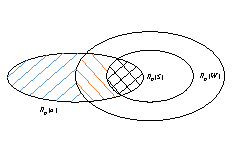
\includegraphics[width=0.8\textwidth]{figures/submodular.pdf}
    \caption{$R_X\left(u\right)$,$R_X\left(S\right)$以及$R_X\left(W\right)$的示意图}
    \label{fig:submodular}
\end{figure}

\begin{proof}\label{pro:submodular}
首先,我们证明对于概率空间中任意的确定的样本点$X$,传播效率函数$T_X\left(\cdot\right)$是具有子模性的。为了证明上述的结论,令$S$和$W$为两个节点集合,且满足$S \subseteq W \subseteq \mathcal{V}$,令$u \in \mathcal{V}$为图$\mathcal{G}$中的任意一个节点。令$\delta\left(u|S\right)$为添加节点$u$至集合$S$后传播效率的边际收益,$\delta\left(u|S\right) = T_X\left(S\cup\left\{u\right\}\right)-T_X\left(S\right)$。然后,我们对$\delta\left(u|S\right)$和$\delta\left(u|W\right)$进行比较。为了方便比较,令$R_X\left(u\right)$表示节点$u$在样本点$X$下的可达节点集合。因为$S \subseteq W$,所以可得$R_X\left(S\right) \subseteq R_X\left(W\right)$。当节点$u$加入到集合$S$和$W$中时,会出现如图\ref{fig:submodular}三种情况。首先,第一种情况如图中的斜线区域,即对于节点$v \in R_X\left(u\right) \setminus R_X\left(W\right)$。在此种情况下,在加入节点$u$之前,图中不存在从集合$S$或者集合$W$到达节点$v$的通路。因此,可知第一种情况中$\delta\left(u|S\right) = \delta\left(u|W\right)$。第二种情况是图中的反斜线区域,即对于节点$v \in \left( R_X\left(u\right) \cap R_X\left(W\right) \right) \setminus R_X\left(S\right)$。在此种情况下,在加入节点$u$之前,图中存在从集合$W$到节点$v$的通路,但是不存在从集合$S$到节点$v$的通路。在此情况下,可知$\delta\left(u|S\right) \geq \delta\left(u|W\right)$。第三种情况是图中的网状区域,即对于节点$v \in R_X\left(u\right) \cap R_X\left(S\right)$。在此种情况下,在节点$u$前,从集合$S$或者集合$W$都有到节点$v$的通路。因为$S \subseteq W$,$e_{W,v} \geq e_{S,v}>0$,所以在第三种情况下$\delta\left(u|S\right) \geq \delta\left(u|W\right)$也是成立的。综合上述可知,结论$\delta\left(u|S\right) \geq \delta\left(u|W\right)$在任意情况下都是成立的,即$T_X\left(S\cup\left\{u\right\}\right)-T_X\left(S\right) \geq T_X\left(W\cup\left\{u\right\}\right)-T_X\left(W\right)$对于集合$S \subseteq W$是成立的,因此$T_X\left(\cdot\right)$是具有子模性的。而又有$\mathbb{E}_\mathcal{G}\left[T\left(S\right)\right] = \sum\nolimits_X{\Pr\left[X\right] \cdot T_X\left(S\right)}$,即传播效率期望值是概率空间中所有可能样本$X$的加权平均值。一个非负的线性组合不会改变函数的子模性,故传播效率函数的期望$\mathbb{E}_\mathcal{G}\left[T\left(\cdot\right)\right]$也是具有子模性。
\end{proof}

\begin{algorithm}[!ht]
\caption{$greedy(k,T)$}
\label{alg:greedy}
\begin{algorithmic}[1]
	\REQUIRE $k,\mathcal{G},T$
    \ENSURE $S$
    \STATE initialize $S=\emptyset$
    \FOR{$i$ =1 to $k$}
        \STATE select $u=\arg\max_{w \in V \setminus S}\left({\mathbb{E}_\mathcal{G}\left[T\left(S\cup w\right)\right]-\mathbb{E}_\mathcal{G}\left[T\left(S\right)\right]}\right)$
        \STATE $S=S\cup u$
    \ENDFOR
    \STATE \textbf{return} $S$
\end{algorithmic}
\end{algorithm}

根据定理\ref{theo:submodular}我们可知传播效率函数的期望值$\mathbb{E}_\mathcal{G}\left[T\left(\cdot\right)\right]$是单调且子模性的,因此朴素贪心算法(\textit{greedy})能够得到一个$1-1/\mathsf{e}$的近似最优解。朴素贪心算法的过程如算法\ref{alg:greedy}所示。算法的流程如下,需要求解的种子节点集合$S$首先置为空集。其次,遍历所有节点,选择传播效率期望值边际收益最大的节点$u$加入到集合$S$中。然后,重复第二步直到集合$S$的大小等于$k$。

此外,由于传播效率期望值具有子模性,因此惰性计算技术\upcite{minoux1978accelerated}可以用来提升朴素贪心算法的性能。惰性计算能够极大地减少模拟评估的次数而不改变贪心算法的的输出。正如惰性计算的名字,该方法的核心思想是尽可能地避免不必要的模拟评估。给定一个单调且子模性的函数$f$,令$f\left(u|S\right)$为集合$S$加入节点$u$后的边际收益,即$f\left(u|S\right) = f\left( S \cup \left\{u\right\} \right) - f\left( S \right)$。假设第$i$轮迭代贪心算法得出的种子节点集合为$S$,且我们对节点$u \in \mathcal{V} \setminus S$的边际收益$f\left(u|S\right)$进行了计算。在更早的迭代中,种子节点集合为$S' \subset S$,且我们计算了节点$w \in \mathcal{V} \setminus S'$的边际收益$f\left(w|S'\right)$。那么当$f\left(w|S'\right) \leq f\left(u|S\right)$时,根据子模性可知$f\left(w|S\right) \leq f\left(w|S'\right) \leq f\left(u|S\right)$。这就是说,在第$i$轮迭代中,节点$w$不可能成为最大化传播效率的节点,因此计算$f\left(w|S\right)$是没有意义的。上述的思想可以通过一个优先队列来实现,如算法\ref{alg:lazygreedy}所示,称之为\textbf{惰性贪心}(\textit{lazy greedy})算法。

\begin{algorithm}[!ht]
    \caption{$LazyGreedy(k,T)$}
    \label{alg:lazygreedy}
    \begin{algorithmic}[1]
    \STATE initialize $S=\emptyset$, priority queue $Q=\emptyset$, iteration $i=1$
    \FOR{$j=1$ to $n$}
        \STATE $u.mg=T\left(u|\emptyset\right)$, $u.i=1$
        \STATE put $u$ into $Q$ with $u.mg$ as the key
    \ENDFOR
    \WHILE{$i \leq k$}
        \STATE pop the top element $u$ of $Q$
        \IF{$u.i = i$}
            \STATE $S = S \cup \left\{u\right\}$, $i=i+1$
        \ELSE
            \STATE $u.mg=T\left(u|S\right)$,  $u.i=i$ 
        \ENDIF
    \ENDWHILE
    \STATE \textbf{return} $S$
    \end{algorithmic}
\end{algorithm}

算法的具体实现过程如下。对于每一个节点$u$,我们为之设计一种结构体,包含两个域值$u.mg$以及$u.i$。其中$u.mg$表示最新一次迭代将节点$u$加入集合$S$时的传播效率期望值边际收益,$u.i$表示$u.mg$更新时的迭代轮数。初始化时,我们对所有节点$u$计算$T\left(u|\emptyset\right)$作为$u.mg$加入优先队列$Q$中,以$u.mg$作为队列的键,此时所有的$u.i=1$。此后的每一轮迭代,我们选择队列$Q$的队首(具有最大的边际收益)的节点$u$进行检查。如果$u.i=i$,即节点$u$确实是第$i$迭代时加入到种子节点集合$S$中的边际收益最大的节点,则将节点$u$加入到种子节点集合$S$中。如果$u.i \neq i$,则更新$u.mg$为$T\left(u|S\right)$,更新$u.i$为当前的迭代轮数,然后将节点$u$插入回优先队列$Q$中。

惰性贪心算法极大地减少了无效模拟评估的次数。Leskovec等人\upcite{leskovec2007cost}通过实验证明该算法对影响力最大化问题的速度提升了近700倍。对于传播效率最大化问题,由于传播效率函数的单调性和子模性,惰性贪心算法也能减少无效模拟评估次数,从而进行加速。

由定理\ref{theo:sharpHard}可知,直接计算传播效率期望值是很困难的。许多相关的工作\upcite{leskovec2007cost,goyal2011celf++,chen2009efficient}在贪心算法的框架下对此类问题进行了改进。然而,这些改进算法仍然不够高效。另一方面,启发式的算法能够解决效率问题,但是不能提供理论上的性能保证。本节借鉴了Borgs等人\upcite{borgs2014maximizing}的反向传播采样思想来解决传播效率最大化问题。

\begin{algorithm}[!ht]
    \caption{$RES$($k$,$r$,$T'\left(\cdot\right)$)}
    \label{alg:res}
    \begin{algorithmic}[1]
    \STATE {initialize $\mathcal{H}=\left(\mathcal{V}, \emptyset \right)$}
    \FOR{$i=1$ to $r$}
        \STATE{stochastically select a node $v \in \mathcal{V}$ uniformly}
        \STATE{generate $z_i = RR\left(v\right)$}
        \STATE{calculate $e_{u,v} = \frac{1}{t_{u,v}+1}$ for $u \in RR\left(v\right)$}
        \STATE{add $z_i$ to the edge set $\mathcal{Z}$ of $\mathcal{H}$}
    \ENDFOR
    \STATE{initialize $S=\emptyset$}
    \FOR{$j=1$ to $k$}
        \STATE{$w = \arg\max_{v \in \mathcal{V}}\left(T'\left(S \cup v\right) - T'\left(S\right)\right)$}
        \STATE{add $w$ to $S$}
        \STATE{remove $w$ from $\mathcal{V}$}
    \ENDFOR
    \STATE {\textbf{return:} $S$}
    \end{algorithmic}
\end{algorithm}

如算法\ref{alg:res}所示,我们称之为\textbf{反向效率采样}(\textit{Reverse Efficiency Sampling}),算法的流程可描述如下。反向效率采样算法按照两步进行。第一步是根据图$\mathcal{G}$建立超图$\mathcal{H}=\left(\mathcal{V}, \mathcal{Z} \right)$,其中$\mathcal{V}$是与图$\mathcal{G}$相同的节点集合,$\mathcal{Z}$是超边集合。每一条超边$z_i \in \mathcal{Z}$代表一个反向可达集合$RR\left(v\right)$,其中节点$v \in \mathcal{V}$,是随机等概率选取的。超边$z_i$可以形式化为一个集合$\{u_1, u_2, \cdots, u_j\}$,代表着存在一条从节点$u \in z_i$到节点$v$的通路。我们不断地随机等概率选取节点$v$,然后基于图$\mathcal{G}$生成图$g$,计算反向可达集合$RR\left(v\right)$,即超边$z_i$,然后添加到超边集合$\mathcal{Z}$中。该过程通过模拟图$\mathcal{G}$的反向图中的信息传播过程来实现。在反向图中首先激活节点$v$,然后按照宽度优先搜索来概率性地激活出度边指向的邻居节点。当信息传播过程停止时,被激活的节点集合构成了超图$\mathcal{H}$中的一条边。同时,我们还需要记录超边上每一个节点$u \in z_i$的传播效率$e_{u,v} = \frac{1}{t_{u,v}+1}$。我们重复生成超边的过程来构建超边集合$\mathcal{Z}$直到集合的大小到达预定的值$r$。

在第二步中,我们基于超图$\mathcal{H}$来计算种子节点集合$S$。在这一步中,算法重复地选择当前传播效率边际收益最大的节点$w \in \mathcal{V}$加入到结合$S$中,其中边际效益为$T'\left(S \cup w\right) - T'\left(S\right)$,且$T'\left(S\right) = \sum_{i=1}^r{\frac{1}{t_{S,v_i}+1}}$,$v_i$为第i轮迭代中随机等概率选取的节点,对应的超边为$z_i$。最终,算法得到一个大小为$k$的节点集合$S$。

下一步,我们对算法\ref{alg:res}进行详细地分析。首先,我们可以观察到种子节点集合$S$的传播效率期望值等于$n$倍从集合$S$到节点$u$的传播效率$e_{S,u}$,其中节点$u$从图$g$中随机等概率选取的,图$g$是基于图$\mathcal{G}$生成的实例图。上述现象可表述为如下,
\begin{mytheo}\label{theo:observe}
$\mathbb{E}_{g\sim\mathcal{G}}\left[T_g\left(S\right)\right]=n\Pr\nolimits_{v,g\sim\mathcal{G}}\left[S\cap RR\left(v\right)\neq\emptyset\right]\cdot\frac{1}{d_{S,v}+1}$
\end{mytheo}
\begin{proof}
    \begin{equation*}
        \begin{split}
            \mathbb{E}_{g\sim\mathcal{G}}\left[T_g\left(S\right)\right] & = \sum\limits_{v \in \mathcal{V}}{\Pr\nolimits_{g \sim \mathcal{G}}{\left[ \exists u \in S, v \in R_g \left(u\right) \right] \cdot \frac{1}{d_{S,v}+1}}}\\
            & = \sum\limits_{v \in \mathcal{V}}{\Pr\nolimits_{g \sim \mathcal{G}}{\left[ \exists u \in S, u \in {RR}_g \left(v\right) \right] \cdot \frac{1}{d_{S,v}+1}}}\\
            & = n \Pr\nolimits_{v,g \sim \mathcal{G}}{\left[ \exists u \in S, u \in {RR}_g \left(v\right) \right] \cdot \frac{1}{d_{S,v}+1}}\\
            & = n \Pr\nolimits_{v,g \sim \mathcal{G}}{\left[ S \cap {RR}_g \left(v\right) \neq \emptyset \right] \cdot \frac{1}{d_{S,v}+1}}
        \end{split}
    \end{equation*}
\end{proof}

定理\ref{theo:observe}表示我们可以通过观察事件$S\cap {RR}_g\left(v\right)\neq\emptyset$的概率来计算$\mathbb{E}_\mathcal{G}\left[T\left(S\right)\right]$。超图$\mathcal{H}$中节点$u \in \mathcal{V}$的度即为信息传播模拟过程中成功激活的节点次数。因此,由定理\ref{theo:observe}可知,我们能够基于超图$\mathcal{H}$来计算传播效率期望值。给定种子节点集合$S$与超图$\mathcal{H}$下的传播效率函数如下所示,
\begin{equation}\label{eq:infEffHyper}
    T'\left(S\right)=\sum\limits_{z_i\in\mathcal{Z}}{\frac{1}{t_{S,v_i}+1}}
\end{equation}
其中$S$为种子节点集合,$z_i$为随机等概率选取的节点$v_i$对应的超边。下一步,我们分析在超图$\mathcal{H}$中的传播效率函数期望值$\mathbb{E}_\mathcal{H}\left[T'\left(\cdot\right)\right]$。我们给出定理如下,
\begin{mytheo}\label{theo:hyperSubmodular}
对于在独立级联模型下的一个网络$\mathcal{G}$的任意一个实例,对应生成的超图$\mathcal{H}$中传播效率函数的期望$\mathbb{E}_\mathcal{H}\left[T'\left(\cdot\right)\right]$是具有子模性的。
\end{mytheo}
\begin{proof}
易证$\mathbb{E}_\mathcal{H}\left[T'\left(\cdot\right)\right]$是单调性的,因为将任意节点$u$加入到任意种子节点集合$S$中都不会减少传播效率期望值。为了证明子模性,我们可以先证明$T'\left(\cdot\right)$的子模性。假设种子节点集合$S$与$W$满足$S \subseteq W \subseteq \mathcal{V}$,节点$u \in \mathcal{V}$是超图$\mathcal{H}$中的节点。如果集合$S \cap z \neq \emptyset$,则我们称集合$S$覆盖超边$z$。与定理\ref{theo:submodular}相同,当将节点$u$加入集合$S$与$W$时,将有三种情况。第一种情况是集合$S$与$W$都不覆盖超边$z$,则$T'\left(S \cup u\right) - T'\left(S\right) = T'\left(W \cup u\right) - T'\left(W\right)$,即二者的边际效益相等。第二种情况是集合$S$不覆盖超边$z$,集合$W$覆盖超边$z$。此种情况下$e_{S,v} = 0$,而$e_{W,v} > 0$,故$T'\left(S \cup u\right) - T'\left(S\right) \geq T'\left(W \cup u\right) - T'\left(W\right)$。第三种情况是集合$S$与$W$都覆盖超边$z$。此种情况下由于$S \subseteq W$,所以$e_{S,v} \leq e_{W,v}$,故$T'\left(S \cup u\right) - T'\left(S\right) \geq T'\left(W \cup u\right) - T'\left(W\right)$。所以对于所有情况,我们都能得出结论$T'\left(S \cup u\right) - T'\left(S\right) \geq T'\left(W \cup u\right) - T'\left(W\right)$在独立级联模型下,$S \subseteq W$的情况下是成立的,因此$T'\left(\cdot\right)$是子模性的。而期望是对$T'\left(\cdot\right)$的加权线性求和,故$\mathbb{E}_\mathcal{H}\left[T'\left(\cdot\right)\right]$也是子模性的。
\end{proof}

由于传播效率函数期望值$\mathbb{E}_\mathcal{H}\left[T'\left(\cdot\right)\right]$是单调且子模的,则算法\ref{alg:res}中的反向效率采样算法能够得到一个$\left(1-1/\mathsf{e}-\varepsilon\right)$的近似最优解来解决独立级联模型下的传播效率最大化问题。其中$\varepsilon$与采样的次数$r$以及图$\mathcal{G}$的结构有关。如何计算$\varepsilon$与$r$以及$\mathcal{G}$的关系仍然是一个开放性的问题。下面本节对上述提及的算法的时间复杂度进行分析。其中朴素贪心算法和惰性贪心算法都是基于贪心算法框架下实现的。这一类算法进行$k$轮迭代来选择种子节点集合$S$,每一轮迭代需要对$O\left(n\right)$个节点进行传播效率期望值的估计。而每一次传播效率期望值的估计需要在$r$个生成的实例图$g$上进行$O\left(m\right)$次计算。因此,朴素贪心算法和惰性贪心算法的时间复杂度都是$O\left(knmr\right)$的。但是由于惰性贪心算法基于惰性计算避免了一些不必要的模拟评估,惰性贪心算法在实际运行中比朴素贪心算法的效率要高。相比之下,反向效率采样算法是在另一个框架下设计的。首先,反向传播采样算法生成了$r$条超边,构造了超图$\mathcal{H}$,每生成一条超边需要消耗$O\left(m\right)$的时间,因此生成整个超图$\mathcal{H}$需要消耗$O\left(rm\right)$的时间。然后,算法迭代$k$轮来生成种子节点集合$S$,每一轮迭代需要对$O\left(n\right)$个节点进行模拟估计,每一次模拟估计需要对$r$条超边进行运算,因此计算种子节点集合$S$的时间复杂度为$O\left(knr\right)$。有上述分析可知,反向效率采样的时间复杂度相比于朴素贪心算法和惰性贪心算法要低。

\section{实验分析}
\label{3sec:experiment}
本节设计了若干组实验来验证上述提出的算法。首先,我们介绍实验的设置。其次,我们详细地展示了实验结果,并对其进行分析。本节中的实验基于八核(Intel Xeon 1.80GHz CPU)、64GB内存的机器运行,操作系统为64位 CentOS release 6.7。以上所有算法都是基于Java实现,在JDK 1.8.0\_40环境下编译。
\subsection{实验设置}
\label{3subsec:settings}
本小节介绍实验的设置,包括数据集、传播模型以及算法等。
\begin{table}[!ht]
\centering
\caption{数据集特征}
\label{tab:dataset}
\begin{tabular}{ |c|c|c|c|c| }
\hline
\textbf{数据集} & \textbf{节点数} & \textbf{边数} & \textbf{类型} & \textbf{平均度} \\
\hline
\textit{Facebook} & 4k & 88k & 无向图 & 43.7\\
\hline
\textit{HepPh} & 35k & 422k & 有向图 & 24.4\\
\hline
\textit{Twitter} & 81k & 1.8M & 有向图 & 43.5\\
\hline
\textit{DBLP} & 655k & 2M & 无向图 & 6.1\\
\hline
\end{tabular}
\end{table}

\textbf{数据集},表\ref{tab:dataset}描述了实验所用的数据集,包括脸书(\textit{Facebook})、高能物理论文引用网络(\textit{HepPh})、推特(\textit{Twitter})、计算机科学合作网络(\textit{DBLP})。这些网络都是相关研究中使用频繁的标注数据集,可以从SNAP\upcite{snapnets}网站上下载得到。实验数据集中的网络有着不同大小的网络和特性,因此能够比较好地验证本章提出的算法。实验数据集包括两个无向图以及两个有向图。其中\textit{Facebook}与\textit{Twitter}是社交网络,如果在\textit{Facebook}网络中用户$u$与用户$v$是好友关系或者在\textit{Twitter}网络中用户用户$v$关注了用户$u$,则在对应的图中存在一条从节点$u$到节点$v$的边$e=(u,v)$。网络\textit{HepPh}为arXiv电子出版高能物理论文的引用网络。如果论文$u$引用了论文$v$,则存在一条从节点$u$到节点$v$的边。而在实验中,我们将\textit{HepPh}网络的边调换了顺序来表示论文$v$影响了论文$u$,如果论文$u$引用了论文$v$。网络\textit{DBLP}提供了一个丰富的计算机科学论文领域的合作网络。如果两位作者曾经合作过一篇文章,则图中存在一条连接两位作者的边。以上的四个网络是具有代表性意义的网络,包含了丰富的社交关系,网络的边集合的大小从万级别到百万级别不等。

\textbf{传播模型},在实验中,我们考虑了如下两种传播模型,即\textbf{均匀独立级联模型}(\textit{Uniform Independent Cascade})和\textbf{加权独立级联模型}(\textit{Weighted Independent Cascade})。其中均匀独立级联模型中的节点$u$到节点$v$传播概率$p_{u,v}$设置为一个常数。在本章的实验中,根据相关的研究工作\upcite{chen2009efficient},对所有网络,我们设置经验参数$p_{u,v}=0.01$。而对于加权独立级联模型,传播概率$p_{u,v}$被设置为$\frac{1}{d_v}$,其中$d_v$表示节点$v$的入度。该模型满足$\sum_{u \in \mathcal{V}}{p_{u,v}} = 1$,因此被先前的相关工作广泛使用\upcite{chen2009efficient, tang2014influence, kempe2003maximizing, cheng2013staticgreedy}。

\textbf{算法},本节中将提出的反向效率采样算法与其他的三种方法进行了比较,反向传播采样算法、惰性贪心算法以及\textbf{最大度算法}(\textit{DegreeGreedy})。首先,我们将反向效率采样算法与反向传播采样算法进行对比来展示传播效率最大化问题与影响力最大化问题的区别。然后,我们进行了实验来验证算法的正确性以及效率。\textit{CELF}算法是在不打破近似最优解理论保证下来解决影响力最大化问题的一个加速算法,我们借鉴\textit{CELF}算法的核心思想实现了惰性贪心算法来解决传播效率最大化问题。最大度算法是一个启发式的算法,在每一轮迭代中选择出度最大的节点做为种子节点。上述的反向传播采样算法、惰性贪心算法、最大度算法和我们提出的反向效率采样算法都是基于Java实现的。

\textbf{参数设置},在比较传播效率以及运行时间时,种子节点集合$S$的大小$k$设置为1, 5, 10,
$\cdots$,直到50。对于惰性贪心算法,我们根据之前相关的工作,经验性地设置蒙特卡罗方法的重复模拟次数$r=10,000$。对于反向效率采样算法,我们设置$r=n\log{n}$来得到一个$(1-1/\mathsf{e}-\varepsilon)$的近似最优解,其中$\varepsilon$与$r$以及网络相关。在所有实验中,我们都重复算法5次,记录其平均值作为实验结果。

\subsection{相似度对比}
\label{subsec:compare}
\begin{figure}[ht]
   \begin{minipage}{0.48\textwidth}
     \centering
     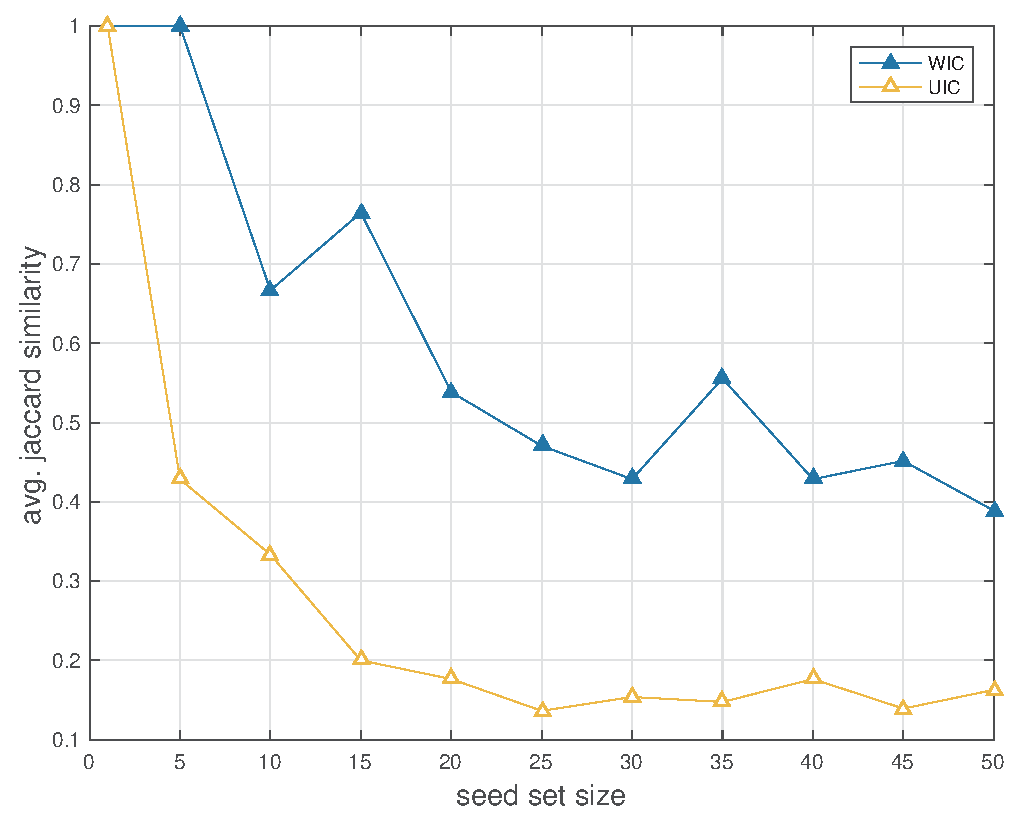
\includegraphics[width=\linewidth]{figures/facebookJaccard.eps}
     \caption{在\textit{Facebook}数据集上不同$k$下的Jaccard相似度对比}
     \label{fig:facebookJaccard}
   \end{minipage}
   \hfill
   \begin {minipage}{0.48\textwidth}
     \centering
     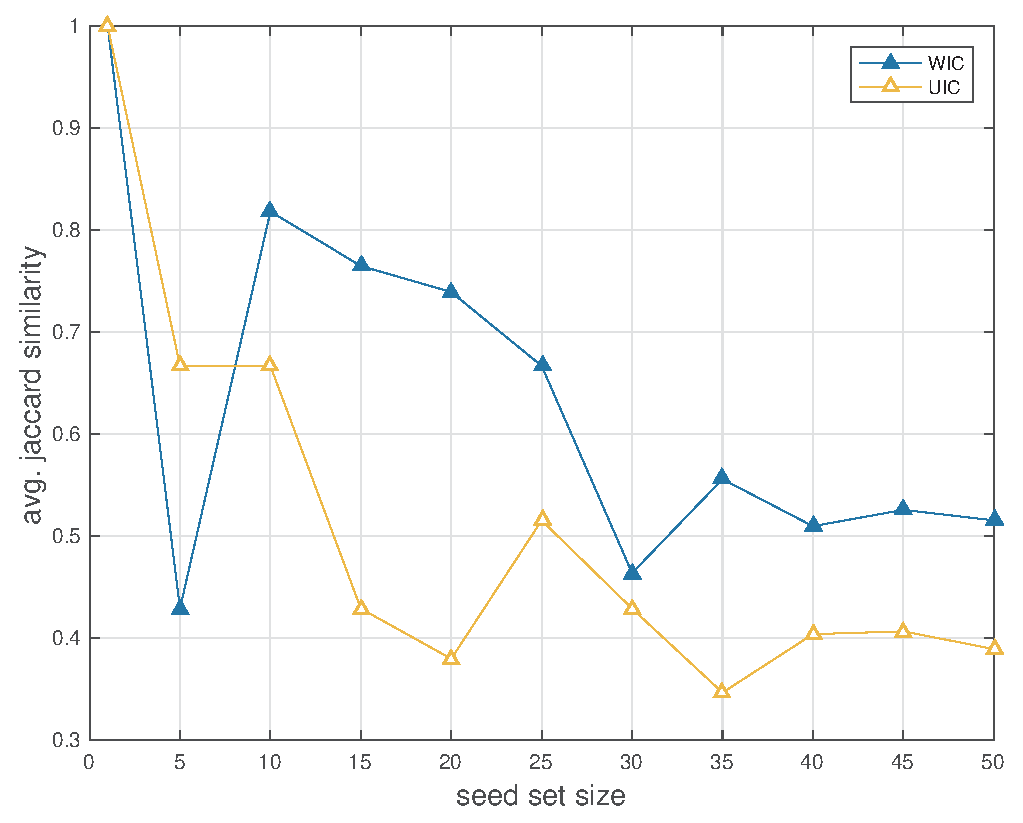
\includegraphics[width=\linewidth]{figures/hepPhJaccard.eps}
     \caption{在\textit{HepPh}数据集上不同$k$下的Jaccard相似度对比}
     \label{fig:hepPhJaccard}
   \end{minipage}
   \\
   \begin{minipage}{0.48\textwidth}
     \centering
     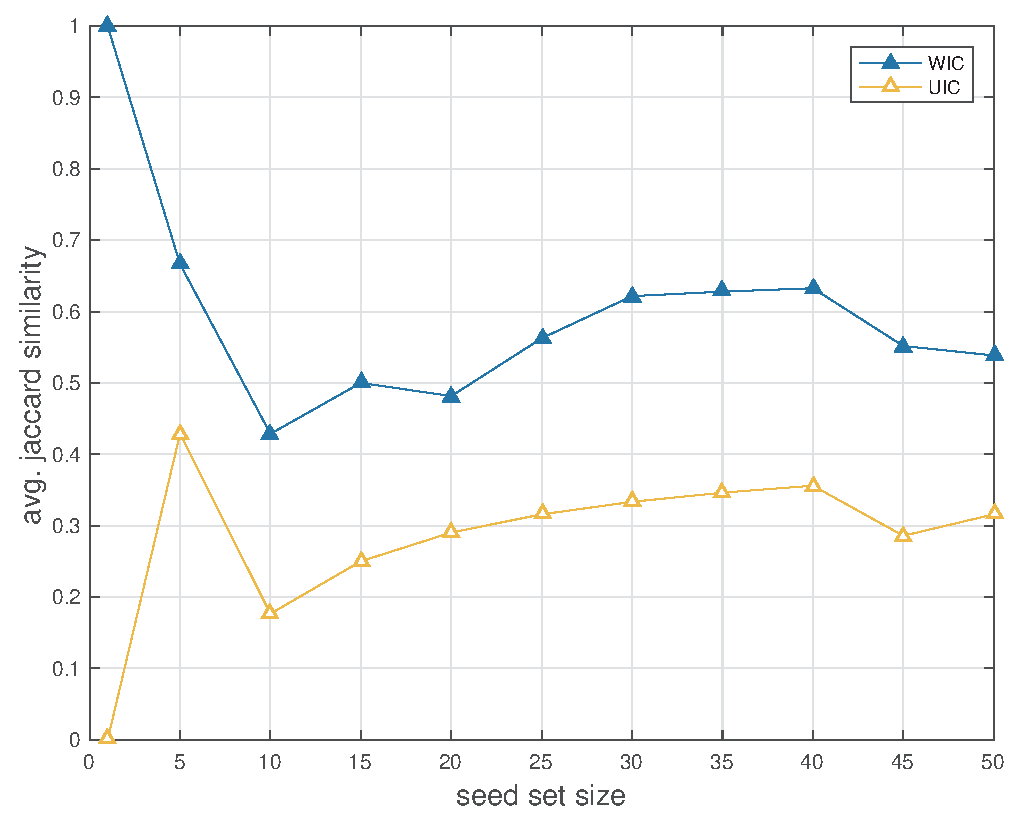
\includegraphics[width=\linewidth]{figures/twitterJaccard.eps}
     \caption{在\textit{Twitter}数据集上不同$k$下的Jaccard相似度对比}
     \label{fig:twitterJaccard}
   \end{minipage}
   \hfill
   \begin {minipage}{0.48\textwidth}
     \centering
     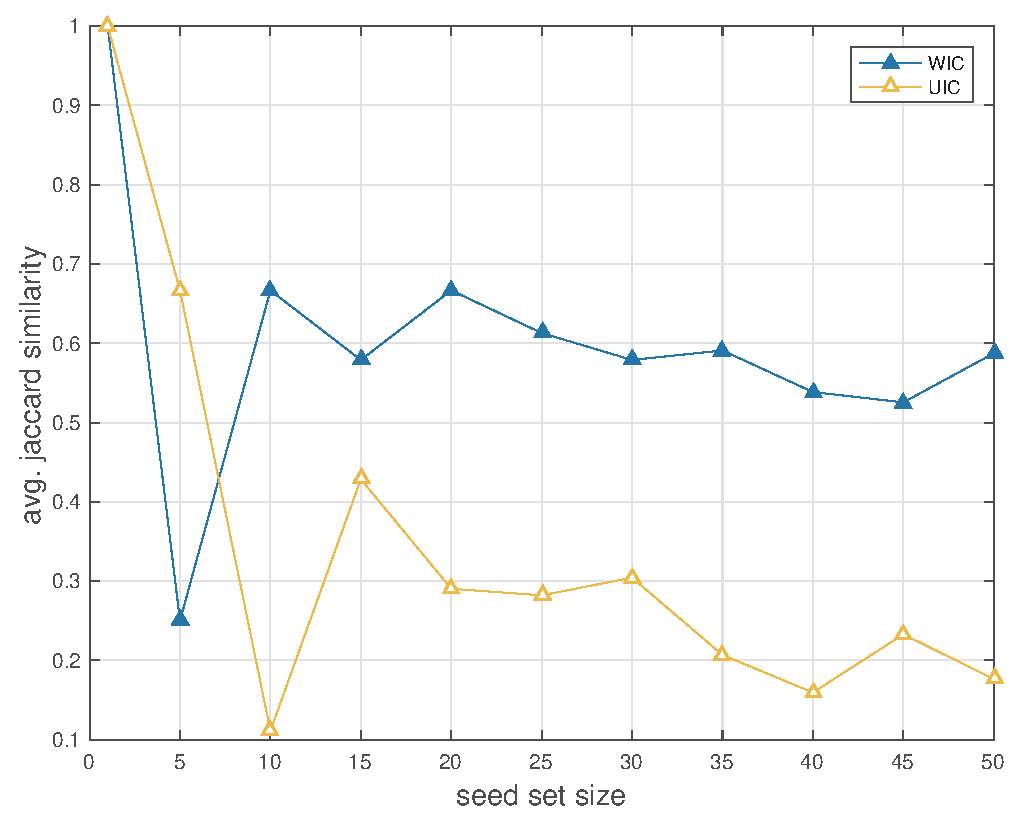
\includegraphics[width=\linewidth]{figures/dblpJaccard.eps}
     \caption{在\textit{DBLP}数据集上不同$k$下的Jaccard相似度对比}
     \label{fig:dblpJaccard}
   \end{minipage}
\end{figure}

第一组实验将反向效率采样算法与反向传播采样算法进行对比,来说明传播效率最大化问题与影响力最大化问题的区别。令反向效率采样算法求解最大化传播效率期望值得到的种子节点集合为$S$,反向传播采样算法求解最大化影响力期望值得到的种子节点集合为$S'$。我们可得到不同$k$下,集合$S$与集合$S'$之间的\textbf{Jaccard相似度}。令$J(S,S')$表示集合$S$与集合$S'$之间的Jaccard相似度,可形式化如下,
\begin{equation}\label{eq:jaccard}
    J(S,S') = \frac{\vert S \cap S' \vert}{\vert S \cup S' \vert}
\end{equation}
其中$\vert S \cap S' \vert$表示集合$S$与集合$S'$的交集大小,$\vert S \cup S' \vert$表示集合$S$与集合$S'$的并集大小。实验结果如图\ref{fig:facebookJaccard}至图\ref{fig:dblpJaccard}所示。从实验结果可知,在$k$较小的时候,例如$k=1$时,Jaccard相似度相似度是不稳定的。在$k=1$的情况下,\textit{Facebook}, \textit{HepPh} and \textit{DBLP}网络中的$S=S'$,而\textit{Twitter}网络中的$S \neq S'$。由此可知,当$k$比较小的时候,使得网络有最大影响力期望值的节点也可能是使得网络有最大传播效率期望值的节点。当$k$比较小的时候,大部分节点处于未激活状态,能够激活尽可能多的节点也许就能获得更大的传播效率。随着$k$的增加,例如超过10以后,在均匀独立级联模型和加权独立级联模型下的$J(S,S')$值变得相对稳定。在均匀独立级联模型中$J(S,S')$约等于0.2,在加权独立级联模型中$J(S,S')$约等于0.5。因此,我们可知传播效率最大化问题的种子节点集合与影响力最大化问题的种子节点集合并不是相同的,即传播效率最大化问题与影响力最大化问题是两个不同的问题。

\subsection{算法精确度对比}
\label{subsec:accuracy}
\begin{figure}[!ht]
   \begin{minipage}{0.48\textwidth}
     \centering
     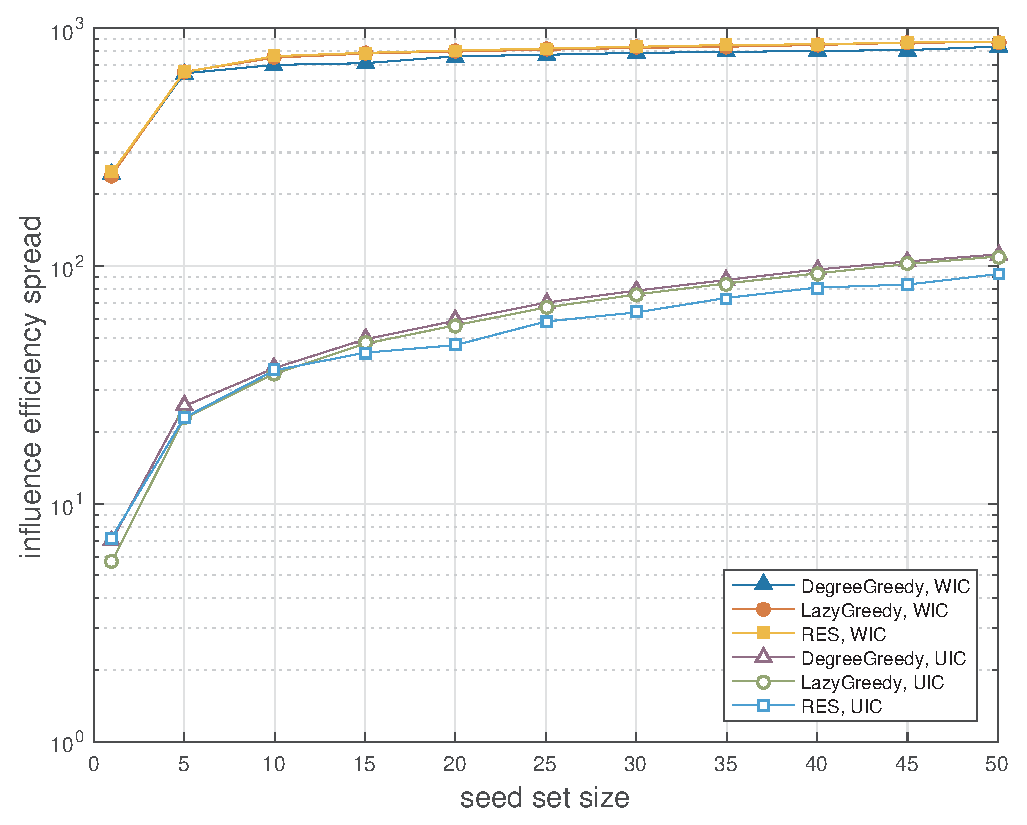
\includegraphics[width=\linewidth]{figures/facebookEff.eps}
     \caption{在\textit{Facebook}数据集上不同$k$下的传播效率对比}
     \label{fig:facebookEff}
   \end{minipage}
   \hfill
   \begin {minipage}{0.48\textwidth}
     \centering
     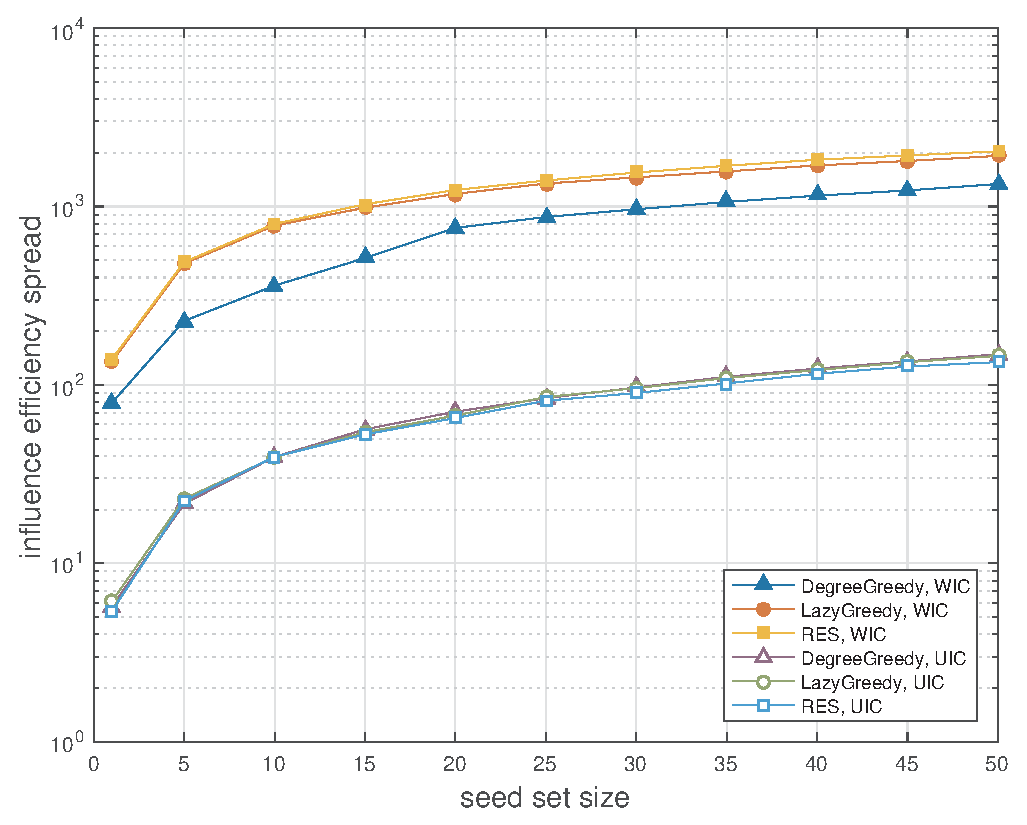
\includegraphics[width=\linewidth]{figures/hepPhEff.eps}
     \caption{在\textit{HepPh}数据集上不同$k$下的传播效率对比}
     \label{fig:hepPhEff}
   \end{minipage}
   \\
   \begin{minipage}{0.48\textwidth}
     \centering
     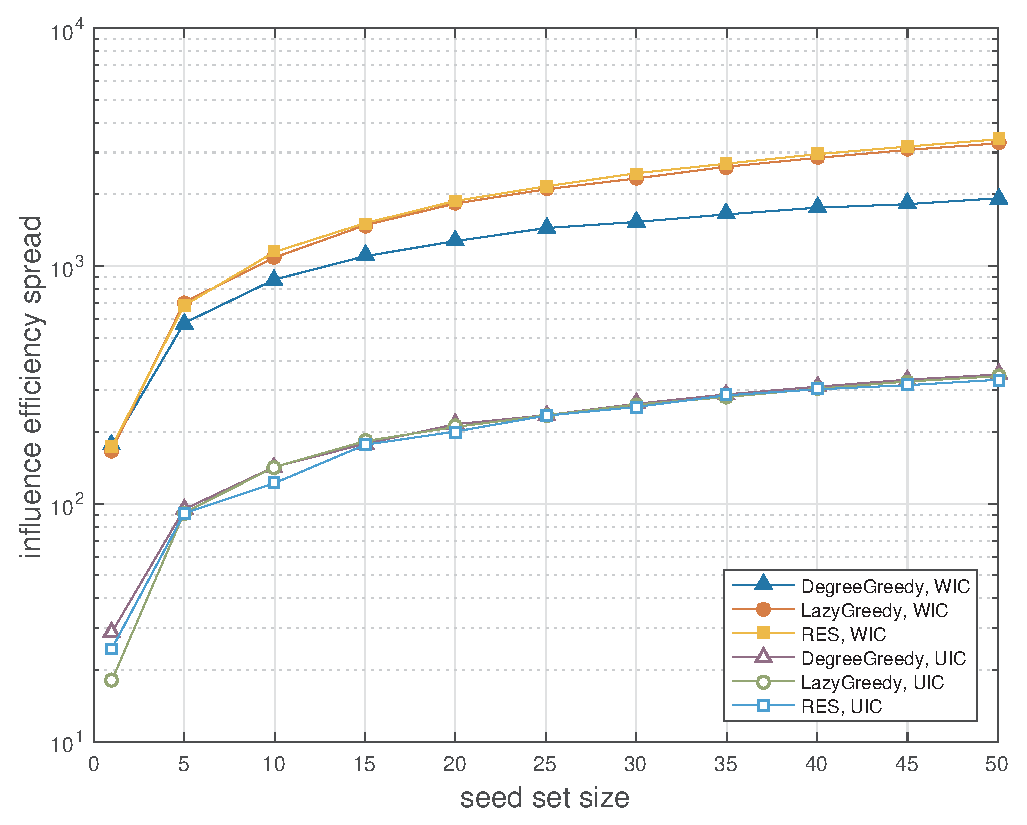
\includegraphics[width=\linewidth]{figures/twitterEff.eps}
     \caption{在\textit{Twitter}数据集上不同$k$下的传播效率对比}
     \label{fig:twitterEff}
   \end{minipage}
   \hfill
   \begin {minipage}{0.48\textwidth}
     \centering
     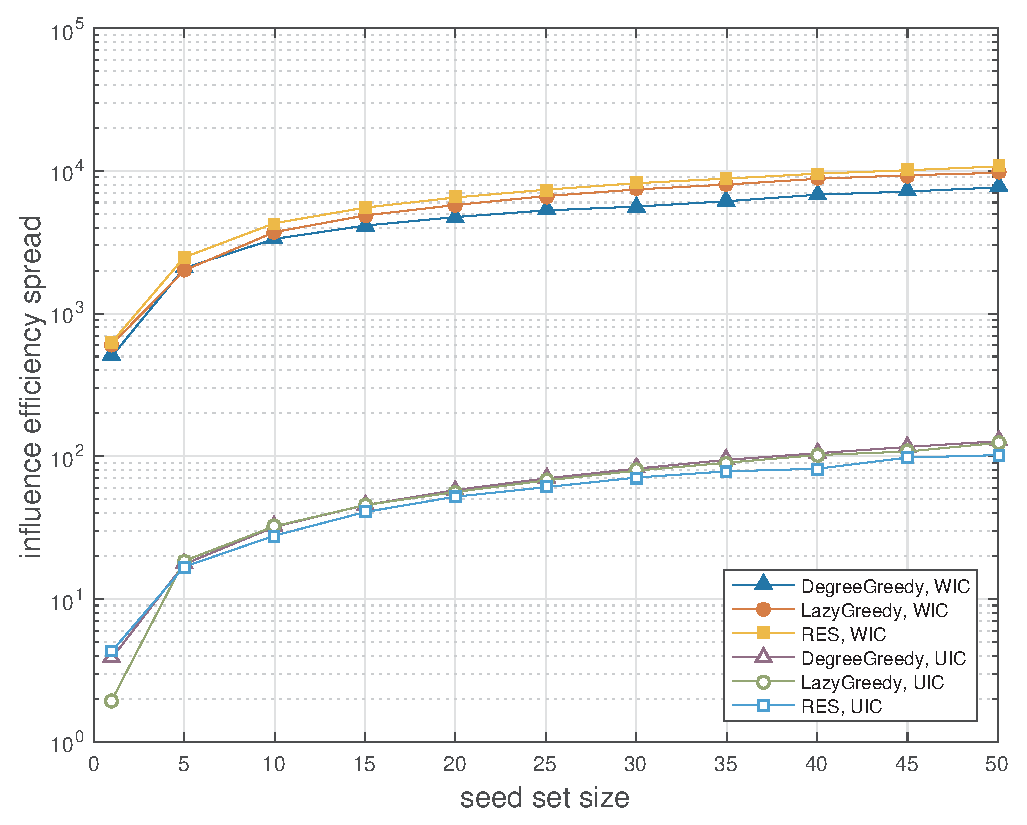
\includegraphics[width=\linewidth]{figures/dblpEff.eps}
     \caption{在\textit{DBLP}数据集上不同$k$下的传播效率对比}
     \label{fig:dblpEff}
   \end{minipage}
\end{figure}

在本小节中,我们计算各种算法得出种子节点集合的传播效率,对比各种算法的精确度。对于结果种子节点集合,我们运行10,000次蒙特卡罗模拟来估计信息传播过程中的传播效率。此外,对于每一个数据集,我们调整种子节点集合大小$k$从1到50来观察不同大小种子节点集合的传播效率。我们在均匀独立级联模型以及加权独立级联模型下进行实验,实验结果如图\ref{fig:facebookEff}至图\ref{fig:dblpEff}所示。如图所示,反向效率采样算法与惰性贪心算法、最大度算法在均匀独立级联模型下各数据集中的传播效率性能相似。这是由于在均匀独立级联模型下不能保证$\sum_{u \in \mathcal{V}}{p_{u,v}} = 1$的成立,且反向效率采样算法得到的近似最优解的近似率不高,所以在某些网络中(例如图\ref{fig:facebookEff}),反向效率采样算法的性能要稍差一些。但是我们可以得知,反向效率采样算法的精确度在最差的情况下(\textit{Facebook}网络)与最好结果相差少于17\%,不会相差一个数量级。在加权独立级联模型下,反向效率采样算法在各数据集中的精确度都是最高的,并且与惰性贪心算法的精确度相似,而最大度算法的精确度相比较低。例如在图\ref{fig:twitterEff}中$k=50$的情况下,最大度算法与反向效率采样算法的精确度相差56.5\%,即最大度算法得出种子节点集合的传播效率只有反向效率采样算法的一半左右。

由上述在均匀独立级联模型以及加权独立级联模型下各数据集上的实验结果可知,反向效率采样算法和惰性贪心算法都有理论上的精确度保证,性能优于启发式算法,例如最大度算法。

\subsection{运行时间对比}
\label{subsec:runningTime}
\begin{figure}[!ht]
   \begin{minipage}{0.48\textwidth}
     \centering
     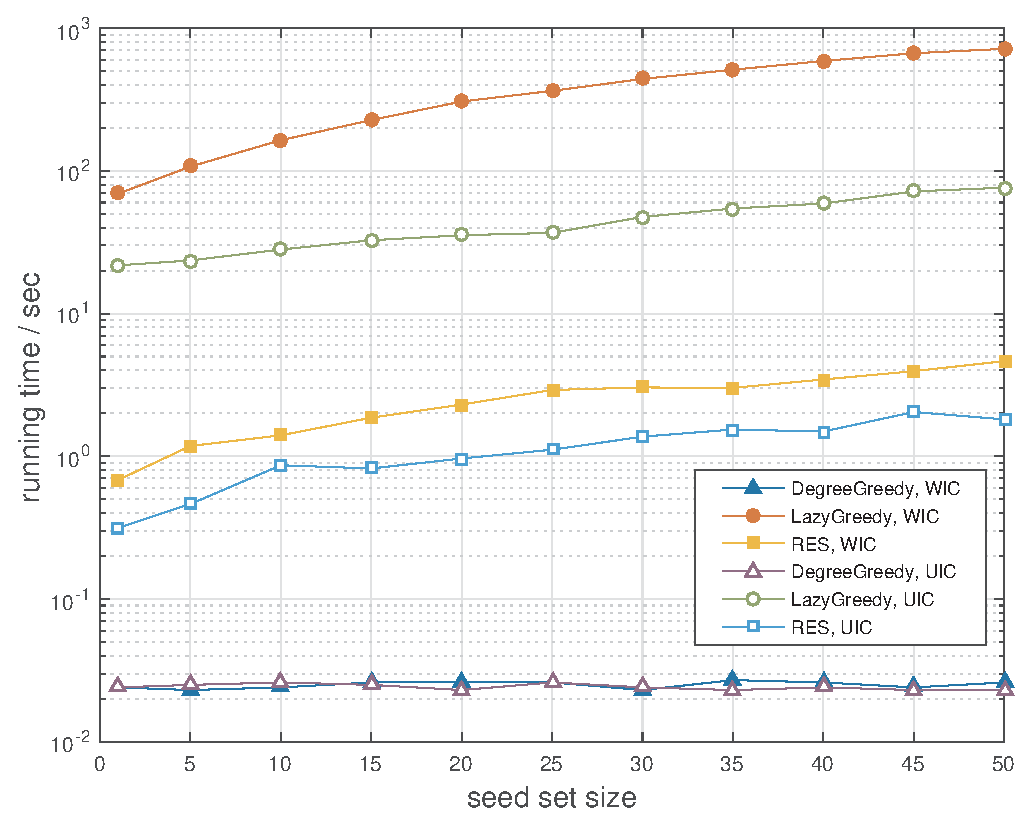
\includegraphics[width=\linewidth]{figures/facebookTime.eps}
     \caption{在\textit{Facebook}数据集上不同$k$下的运行时间对比}
     \label{fig:facebookTime}
   \end{minipage}
   \hfill
   \begin {minipage}{0.48\textwidth}
     \centering
     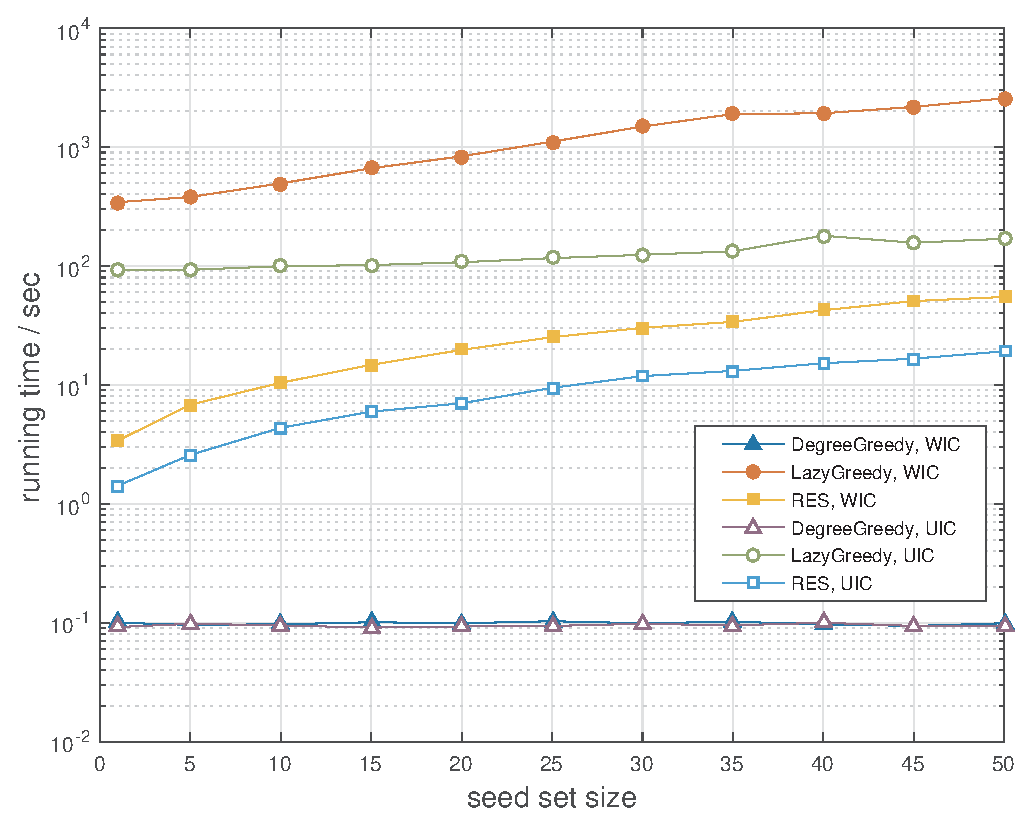
\includegraphics[width=\linewidth]{figures/hepPhTime.eps}
     \caption{在\textit{HepPh}数据集上不同$k$下的运行时间对比}
     \label{fig:hepPhTime}
   \end{minipage}
   \\
   \begin{minipage}{0.48\textwidth}
     \centering
     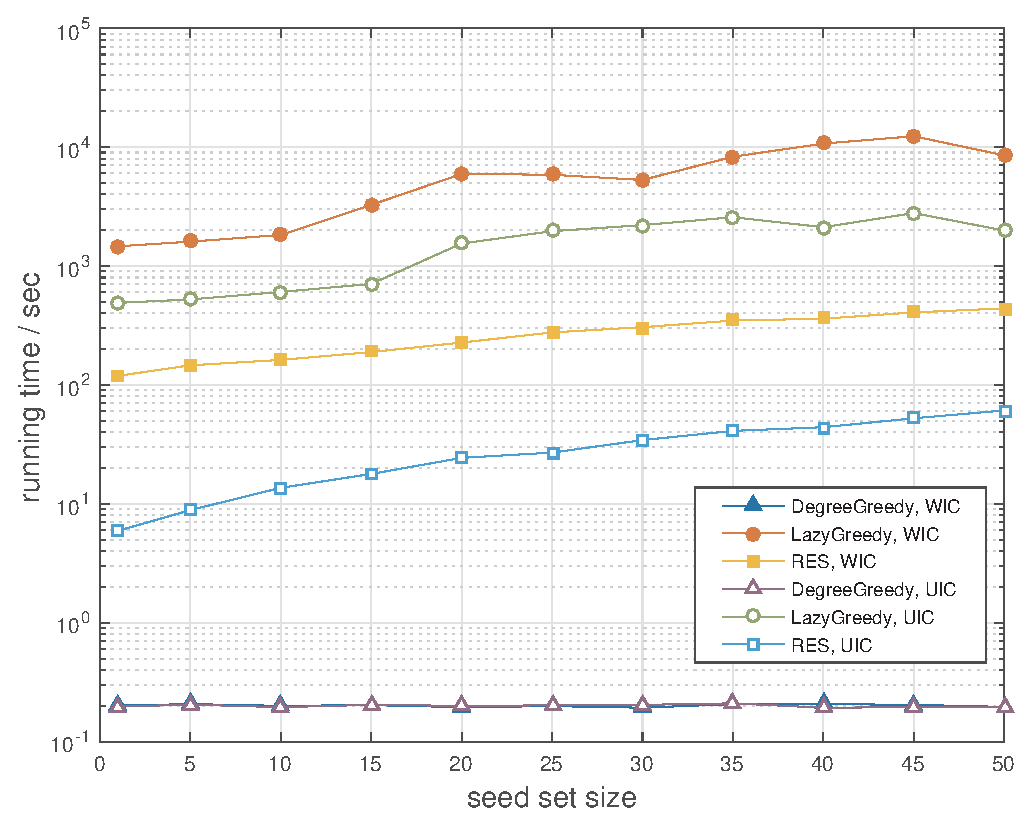
\includegraphics[width=\linewidth]{figures/twitterTime.eps}
     \caption{在\textit{Twitter}数据集上不同$k$下的运行时间对比}
     \label{fig:twitterTime}
   \end{minipage}
   \hfill
   \begin {minipage}{0.48\textwidth}
     \centering
     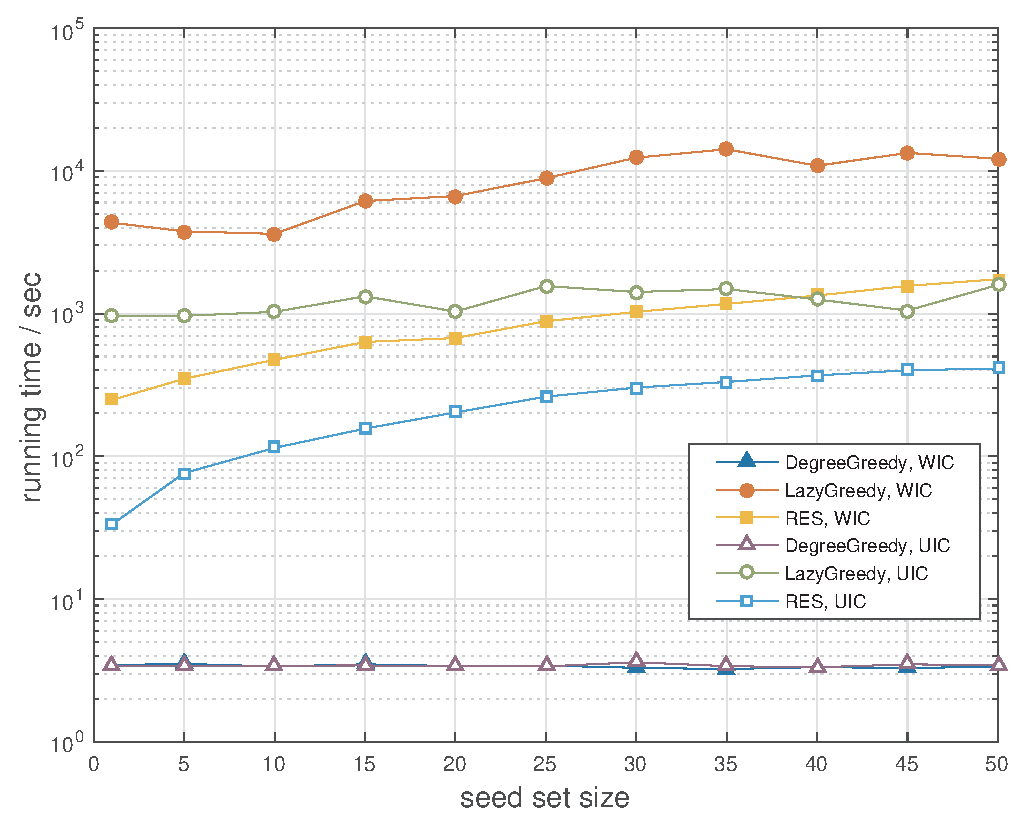
\includegraphics[width=\linewidth]{figures/dblpTime.eps}
     \caption{在\textit{DBLP}数据集上不同$k$下的运行时间对比}
     \label{fig:dblpTime}
   \end{minipage}
\end{figure}

本小节我们对各算法的运行时间进行对比实验。为了验证反向效率采样算法的效率,我们在均匀独立级联模型以及加权独立级联模型下各数据集上不同$k$的情况下,与惰性贪心算法以及最大度算法进行实验对比,结果如图\ref{fig:facebookTime}至图\ref{fig:dblpTime}。如图所示,在均匀独立级联模型以及加权独立级联模型下,反向效率采样算法相比惰性贪心算法都能提高一个数量级的效率。而最大度算法是一种启发式的算法,因此运行时间最少,且不随$k$的变化而变化,但是如第\ref{subsec:accuracy}小节所示,该算法不能提供性能的保证。因为最大度算法算法简单,本小节利用该算法来作运行时间的一个下限基准。从图中我们可以得出,反向效率采样算法和惰性贪心算法的运行时间都随着$k$的增加而增加,其中惰性贪心算法运行时间的增长速率高于反向效率采样算法。例如,在图\ref{fig:twitterTime}中在$k=1$时,惰性贪心算法的运行时间约为反向效率采样的10倍,在$k=50$时,增长为约20倍。因此,反向效率采样算法的效率优于其他的算法。

\subsection{可扩展性}
\label{subsec:scalability}
\begin{figure}[ht]
    \centering
    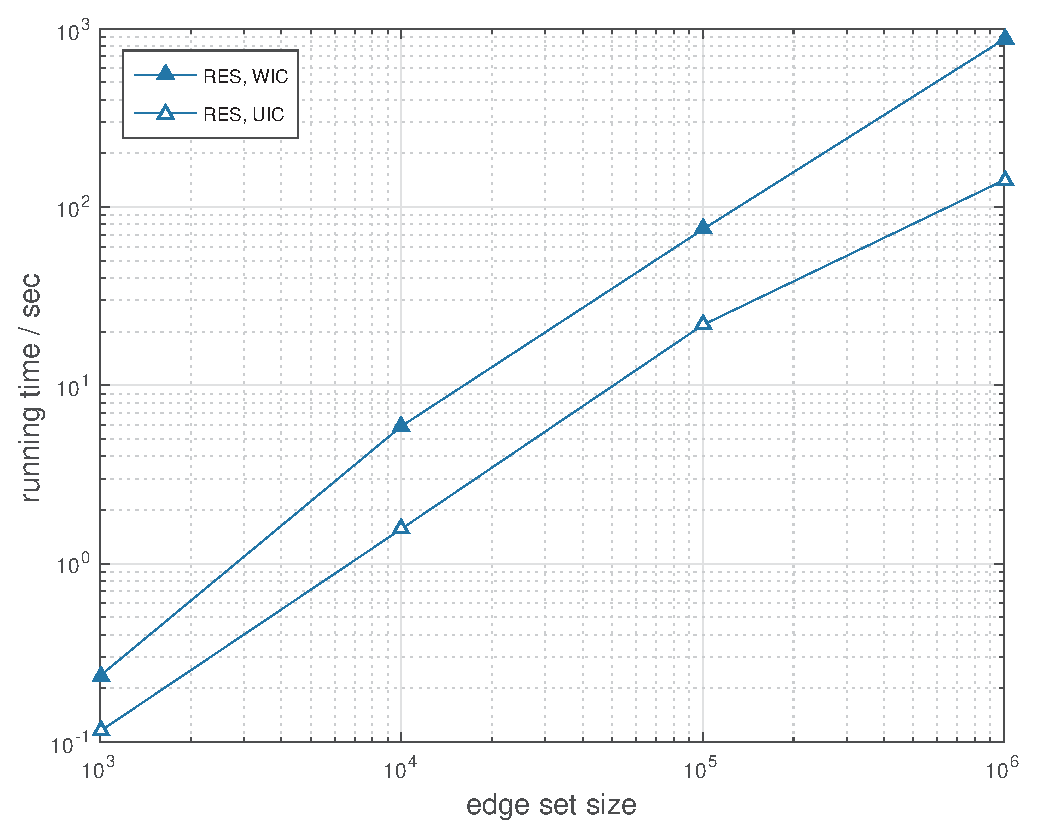
\includegraphics[width=0.5\textwidth]{figures/resScalability.eps}
    \caption{反向效率采样算法的可扩展性}
    \label{fig:scalability}
\end{figure}

本小节进行了反向效率采样算法的可扩展性实验。实验使用\textit{DBLP}网络来生成各种大小的子图。生成过程如下所示。首先,我们随机地选取图中的一个节点,然后做宽度优先搜索来添加边到子图中,该过程直到子图的大小满足要求时停止。如果宽度优先搜索过程在子图大小没有满足前就停止了,那么在重新随机地选择一个不在目前子图中的节点,继续进行宽度优先搜索,重复上述过程直到满足要求。利用该方法,我们可以得到各种大小的子图。本小节的实验中,我们令子图的边的大小从$m=1,000$到$m=1,000,000$变化,然后运行反向效率采样算法,记录运行的时间。在均匀独立级联模型以及加权独立级联模型下的实验结果如图\ref{fig:scalability}所示。由图可知,随着图大小的增长,运行时间的增长是线性的。因此,反向效率采样算法是可扩展的。
\section{本章小结}
\label{3sec:conclusion}
为了更好地理解网络中的传播效率,本章将信息传播过程中的传播时延考虑在内,提出了一个新的问题,传播效率最大化问题。该问题的目的在于最大化网络中的传播效率期望值。然后,我们证明了在独立级联模型下,传播效率最大化问题是一个NP-hard的问题,而且计算传播效率的过程是一个\#P-hard的问题。为了解决该问题,我们证明了在独立级联模型下,传播效率函数的期望值是单调且子模性的。基于上述的性质,我们设计了三种算法来解决该问题。最后,我们在真实的数据集上进行了一系列的实验来验证所提出的算法。实验结果表明了传播效率最大化问题与影响力最大化问题的不同,证明了提出的算法的正确性和有效性。本章所研究的内容对充分理解信息传播过程有着一定的帮助。


\chapter{基于卷积神经网络的文本分类研究}
近年来,深度学习(Deep Learning)在计算机视觉\upcite{krizhevsky2012imagenet}以及语音识别\upcite{graves2013speech}等方面取得了显著的成果。在自然语言处理领域,深度学习方法对于语义理解以及文本表示等方面也进行了技术的革新,相关的工作包含基于神经语言模型进行词向量表示的学习\upcite{bengio2003neural,yih2011learning,mikolov2013distributed}以及基于已学习的词向量模型进行文本分类\upcite{collobert2011natural}等。在社交网络信息传播分析中,文本分类的研究一直是社交网络数据分析与挖掘的基础和热点。社交网络中海量的用户生成数据(User-Generated Content)提供了话题种类繁多的信息。如何实现社交网络中的文本自动分类是一个极具挑战的任务。

由于社交网络中文本的数据海量性、话题多样性以及数据稀疏性等特点,传统的文本分类技术的效率将变低,无法很好的解决文本自动分类任务。例如词袋模型(Bag-of-Words Model)的词向量维度将随着社交网络中的词组数量增加而增加,词向量的稀疏性将给语义模型的训练带来精确性上的降低,并且使得模型训练的时间开销增加。卷积神经网络(Convolutional Neural Networks)将卷积核应用到局部特征上来进行语义的处理\upcite{lecun1998gradient}。该技术首先是用于计算机视觉领域,同时CNN模型近年来在自然语言处理领域上也取得了很好的效果,例如语义分析\upcite{yih2014semantic}、查询检索\upcite{shen2014learning}、语句建模\upcite{kalchbrenner2014convolutional}以及其他的自然语言处理任务\upcite{collobert2011natural}。本章针对传统文本分类方法的不足,利用深度学习的方法对文本分类问题进行处理,对文本中语句的重要性进行排序,提取核心语句集合作为文本的语义表示,训练设计的CNN模型参数,实现文本的自动分类。

本章主要的工作可以总结如下。首先,结合卷积神经网络的特性,本章提出了一个面向社交网络的文本自动分类框架。其次,本章提出了一个核心语句提取的算法,在保证文本语义的同时降低了计算的复杂度,而且保留了文本语句中的词序。然后,本章利用外部语料库训练好的词向量模型对文本进行表示,将文本转换成一个语义矩阵,利用社交网络中标注好的预料对CNN模型参数进行训练,实现文本自动分类。最后,本章在真实数据集上进行了实验,与传统的方法进行对比,验证了算法的有效性。

本章的内容组织如下:第\ref{sec3:motivation}节介绍了研究动机,讨论了传统文本分类方法的不足以及深度学习方法对于文本分类的帮助。第\ref{sec3:definition}节介绍了相关定义,对本章中相关概念和所提出的问题进行了符号化的定义。第\ref{sec3:method}节介绍了方法描述,详细地阐述了本章所提出的框架以及相关算法的详细过程。第\ref{sec3:experiment}节进行了实验分析,设计了一系列的实验,验证了本章所提出的方法,并对实验结果进行了分析。最后,第\ref{sec3:conclusion}节对本章的内容进行了总结。
\section{研究动机}
\label{sec3:motivation}
随着各类社交媒体的蓬勃发展,人们所需要面对的信息量呈指数式爆炸增长。信息中包含各种各样的内容和话题,信息的呈现方式多样,包括文字、图片、视频以及音频等等。这对人们处理信息的能力提出了新的挑战和要求。在社交网络的传播分析中,文本分类研究是数据分析与挖掘的基础。社交网络中,人人都可以是信息的生产者、传播者和接收者。与传统的媒体相比,这种形式极大地加速了信息的传播速率。而人们很难及时处理扑面而来的海量信息,将会淹没在信息洪流之中,从而无法有效地获取自身所感兴趣的、对自身有用的信息。因此,在大数据时代,如何处理海量数据的文本分类问题是一个极具挑战性的任务。

传统的数据挖掘对于分类问题已经进行了长期的研究,提出了许多实用的算法来解决分类问题。例如支撑向量机(Support Vector Machine)算法\upcite{cortes1995support},该算法通过寻找一个超平面来分割不同类别的数据,从而进行分类。又例如k近邻(k-Nearest Neighbors)算法\upcite{hastie1996discriminant},该算法的指导思想是“近朱者赤,近墨者黑”,一个待分类的样本将由特征空间中离它最近的k个样本的类别所决定。其余分类算法还包括朴素贝叶斯(Naive Bayes)算法、决策树(Decision Trees)算法以及神经网络(Neural Network)模型等等。这些算法在文本分类问题上都具有实用性,但是随着数据量的增长、类别的多样性、数据的稀疏性等问题的出现,算法的性能都有所下降。在信息量急剧增长的社交网络中,需要新的方法来解决文本的分类问题。

随着深度学习技术的发展,各个领域都在利用深度学习来解决其领域内的问题。例如在语音识别方面,Graves等人\upcite{graves2013speech}提出了一种使用循环神经网络(Recurrent Neural Networks)的语音识别技术,该方法结合了多层表示以及长范围上下文的灵活使用来提高循环神经网络的性能。Sainath等人\upcite{sainath2015convolutional}整合卷积神经网络(Convolutional Neural Networks)、LSTM(Long Short-Term Memory)以及深度神经网络(Deep Neural Networks)到一个统一框架中,利用CNN能减少频率变化、LSTM对于时序建模以及DNN将特征映射到更可分空间的特性,提高了语音识别的性能。在目标检测与识别方面,Szegedy等人\upcite{szegedy2015going}针对大规模图像识别问题,通过增加神经网络的深度和宽度,同时保持计算量不变,实现了一个22层的深度神经网络GoogleNet。Erhan等人\upcite{erhan2014scalable}针对目标识别的问题,应用了深度神经网络来进行建模。在机器翻译方面,Sutskever等人\upcite{sutskever2014sequence}提出了一个多层的LSTM网络将输入序列映射为一个指定维度的向量,然后另外一个LSTM网络用来进行解码,实现不同语言之间的机器翻译。Bahdanau等人\upcite{bahdanau2014neural}猜想定长向量是使用深度学习实现机器翻译的瓶颈,基于编码器-解码器的基础架构,提出了一个对于目标词语自动搜索源语句的模型。在语言模型方面,Chelba等人\upcite{chelba2013one}给出了一个新的基础数据集,用于评测统计语言模型,并对几种流行的语言模型进行了评测,RNN相对于其余的语言模型取得了更好的表现。在语法分析方面,Vinyals等人\upcite{vinyals2015grammar}针对自然语言处理中的语法分析问题,提出了一个领域未知关注增强模型,能在人工干预很小的情况下,取得很好的效果。深度学习技术在众多领域都取得了不错的效果,因此,使用深度学习技术来解决文本分类问题是一个可行的方法。

\begin{figure}[!htbp]
  \centering
  % Requires \usepackage{graphicx}
  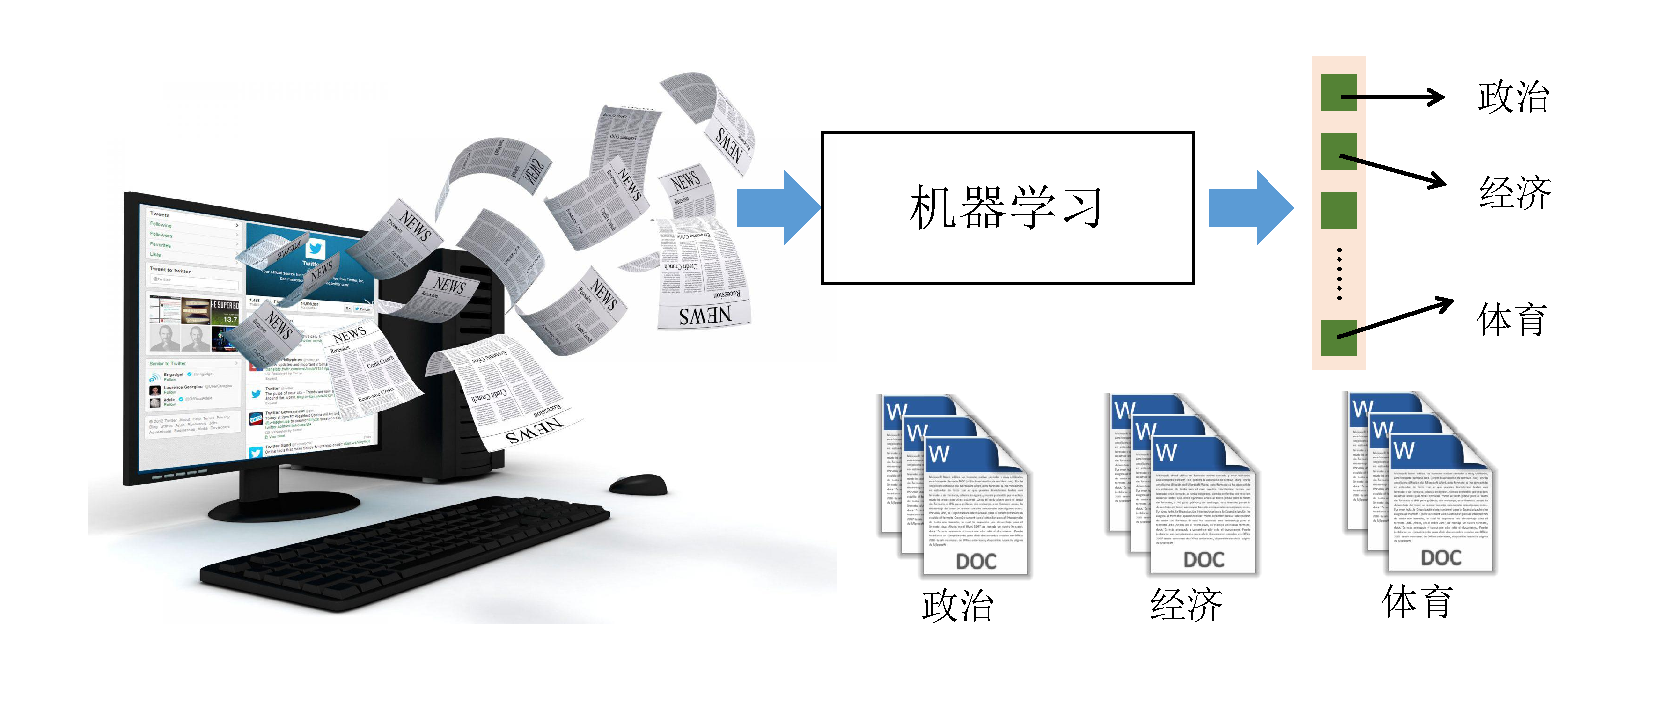
\includegraphics[width=\textwidth]{textClassification}
  \caption{社交网络中文本分类任务示意图}
  \label{fig:textClassification}
\end{figure}

图\ref{fig:textClassification}为社交网络中文本分类任务的示意图。首先,我们从社交媒体中得到文本信息,例如新闻、博客等等。然后,通过机器学习的方法,我们利用标注好的数据来训练模型,得到分类器的参数。最终,利用训练好的分类器对文本的分类进行预测。社交网络中的文本数据量大,话题种类较多,对文本分类突出了新的要求。问题主要集中在如下两方面:
\begin{itemize}
  \item 语言表示模型。社交网络中的信息量随着时间而增加,不断地有新词产生,传统的词袋模型面临着维度爆炸的问题。维度的规模过大而且过于稀疏将限制模型的训练效率,使得难以得到好的效果。
  \item 分类训练模型。社交网络中的文本信息包含着上下文关系,而传统的朴素贝叶斯算法、SVM算法等都是基于统计的方法,丢失了文本的上下文关系,而这些特征对于文本分类问题是有意义的。
\end{itemize}

为了解决上述问题,本章提出了一种结合词向量模型和卷积神经网络的文本分类算法,该算法控制了文本表示的维度,保留了上下文关系的局部特征。首先,本章提出了一种快速的文本摘要提取方法,将长文本信息中的核心语句进行提取。而后,利用外部语料库训练得到的词向量模型,将语句中的词语转换成向量模型。最后,利用核心语句作为一个卷积神经网络的输入,对网络进行训练,最终得到神经网络的参数。在真实数据集上对该算法进行了评估,验证了算法的正确性和有效性。

\section{相关定义}
\label{sec3:definition}
本节首先对社交网络中的文本信息分类问题进行定义,并形式化的将其表述。然后对其中涉及到的概念进行具体的描述。
社交网络中的文本信息分类问题可以描述如下。在社交网络平台中,令$\mathbf{D}$表示信息集合,可以看作为一个文档集合,其中的一条信息定义为$\mathbf{d} \in \mathbf{D}$。社交网络的文本信息属于不同的类别$c \in \mathbf{C}$,其中$c$为某一个主题,$\mathbf{C}$为主题集合。基于以上的描述,社交网络中的文本分类问题可以定义如下,
\begin{defn}[文本分类问题]\label{def:textClassification}
在社交网络中,给定主题类别集合$\mathbf{C}$以及信息集合$\mathbf{D}$,文本分类问题是要解决如何将信息分类到正确的类别中,即将$\mathbf{d} \in \mathbf{D}$自动地分类到正确的$c \in \mathbf{C}$。
\end{defn}

根据定义\ref{def:textClassification}可知,社交网络中的文本分类问题需要解决的两个关键问题如下。首先是语言表示模型,即如何将文本信息进行表示,映射到一个可以用于计算相似度的空间。其次是分类训练模型,即如何设计分类器,利用训练数据集对分类模型进行训练,得到分类器的参数。社交网络平台中文本分类问题可以通过图\ref{fig:textClassificationProblem}来表示。

\begin{figure}[!htbp] % use float package if you want it here
  \centering
  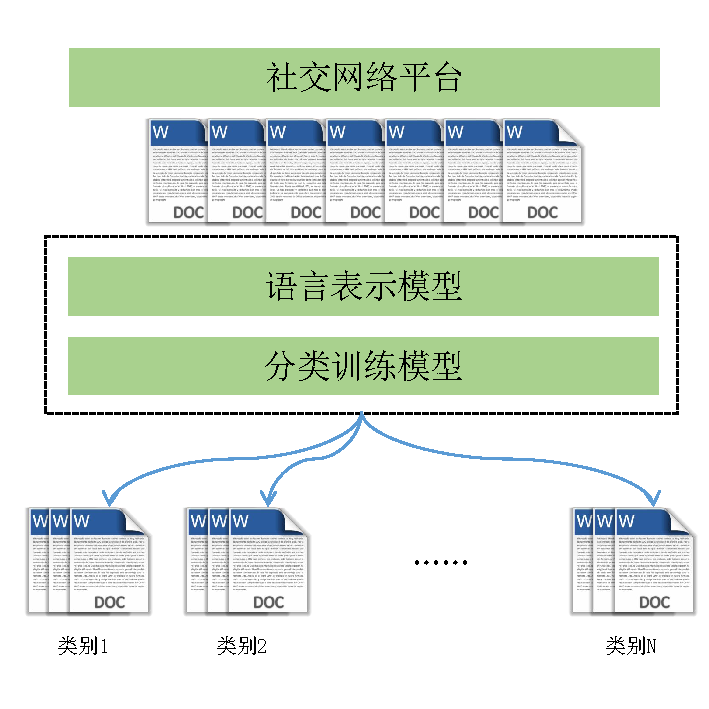
\includegraphics[width=0.5\textwidth]{textClassificationProblem}
  \caption{社交网络平台中文本分类问题}
  \label{fig:textClassificationProblem}
\end{figure}

图中的文档代表着一条信息,每一条信息$\mathbf{d}$都是由语句组成,语句以$\mathbf{s}$表示。一条语句$\mathbf{s}$由词语表示,一个词语可表示为$\mathbf{t}$。词语与词语之间存在着上下文关系,即词序关系。语言表示模型是将文本信息映射到一个可计算的空间的操作,方便文本之间进行相似度的计算。文本信息通过语言表示模型后,作为分类训练模型的输入。分类训练模型通过标注的训练数据集来进行参数的训练,得出分类器,最终对未知数据的类别进行预测。

\section{方法描述}
\label{sec3:method}
在本节中,我们借鉴了Kim的思想\upcite{kim2014convolutional},并且做出了改进,实现了一个基于卷积神经网络的文本分类器。针对社交网络中的长文本信息(例如新闻、长微博等)的话题分类问题,我们设计了一个基于深度学习的框架来解决文本的分类问题。详细的算法将在本节中进行阐述。首先,我们介绍文本摘要算法,该算法用于长文本信息中的关键语句的提取。相对于Mihalcea\upcite{mihalcea2004graph}所提出的基于图排序算法的语句提取算法,我们所提出的文本摘要算法更加的简洁。算法基于词语的tf-idf值来计算语句的重要性,该算法相对耗时短,更加适用于社交网络中长文本的关键语句提取。其次,我们选取top-\textit{k}个语句来作为长文本信息的摘要。这个过程减少了长文本信息的规模,并且消除了其中的大量的噪声语句。然后,基于外部语料库(例如维基百科等),我们建立了一个词向量模型(Word Vector Model)。该模型将关键语句中的词语转换成向量。在这一步骤中,我们仍然保留了语句中的词序顺序关系,即上下文关系。最终,我们利用标注好的数据集来训练所设计的三层卷积神经网络。各个步骤的详细描述在下面的各小节中进行描述。

\subsection{文本摘要提取}
\label{subsec3:abstactExtract}
对于文本摘要提取,其核心的思想是对文本信息中的语句进行排序,遴选出其中最能代表文本主题的语句。这个步骤在整个文本分类中是比较重要的,它能够降低文本信息的规模,消除噪声语句,减少文本分类器的训练时间。社交网络中的长文本信息包含的语句可能会比较多,为了保证文本分类的效率,我们利用文本摘要算法来降低文本中语句的规模。在本小节中,基于词语的tf-idf值,我们实现了一种文本摘要算法来提取长本文信息中的关键语句。语句按照其中词语的tf-idf值进行排序,排序靠前的top-\textit{k}个语句被选择作为该信息的摘要,用来代表信息的核心语义。

我们将社交网络中的长文本信息看作一篇文档$\mathbf{d}$,用$\mathbf{t}$表示文档中的词语。对于某一篇文档$\mathbf{d}_j$中的一个词语$\mathbf{t}_i$,我们定义词语$\mathbf{t}_i$在文档$\mathbf{d}_j$中的词频(Term Frequency)为${\textit{tf}}_{ij}$。词语$\mathbf{t}_i$的逆向文件频率 (Inverse Document Frequency)可以表示成${idf}_i = \log \frac{\vert \mathbf{D} \vert}{1 + \vert \{\mathbf{d} \in \mathbf{D} : \mathbf{t}_i \in \mathbf{d}\}\vert}$,其中$\mathbf{D}$表示整个文档集合,即所有的长文本信息集合。通过这种方法,我们可以得到不同文档中所有词语的tf-idf值。众所周知,词语的tf-idf值能够反映出词语在文档中的重要性。许多已有的工作利用这一特性来进行文本处理,例如词袋模型使用一定数量的具有高tf-idf值的词语来表示整篇文档的语义。但是,词袋模型破坏了语句中的词序,词语的上下文关系在处理过程中没有得到保留,这会造成部分语义信息的丢失。为了解决这个问题,我们期望得到能够代表文档的关键语句,然后以语句的集合来表示文档的语义,这样能够保留文档中的词序关系,即上下文关系。我们进行如下的假设,如果语句中所包含的词语的tf-idf值较高,那么该语句更有可能表示这篇文档的主题思想,即更可能为关键语句。因此,我们选择若干个关键语句来表示整篇文档的语义,从而不破坏文档中的词序关系,保留上下文关系。

本小节中的文本摘要提取方法可以描述为如下。首先,我们定义$\mathbf{s}$为文档中的的一个语句。语句$\mathbf{s}$可以表示成公式(\ref{eq:sentence})所示,
\begin{equation}
\label{eq:sentence}
	\mathbf{s}=\mathbf{t}_1 \oplus \mathbf{t}_2 \oplus \cdots \oplus \mathbf{t}_K
\end{equation}
其中符号$\oplus$为连接符号,表示词语间的词序关系,$K$表示语句$\mathbf{s}$的长度。然后,我们按照语句$\mathbf{s}$中词语的tf-idf值来对语句进行语义重要性的排序。直观地说,如果语句$\mathbf{s}$中所包含的词语的tf-idf值较高,那么语句的排序应当更靠前。值得注意的是,一个长语句所包含的词语将会更多,包含高tf-idf值词语的概率将更大。因此,为了避免长语句的排名更加靠前,引入一个归一化因子来处理语句的长度问题是非常有必要的。定义$I(\mathbf{s}, \mathbf{d}_j)$为语句$\mathbf{s}$在文档$\mathbf{d}_j$中的语义重要性,$I(\mathbf{s}, \mathbf{d}_j)$可以形式化为公式(\ref{eq:importance})所示,
\begin{equation}
\label{eq:importance}
	I(\mathbf{s}, \mathbf{d}_j)=\frac{\sum \nolimits_{\mathbf{t}_i \in \mathbf{s}} {tf}_{ij}\cdot{idf}_i }{\log \left(\vert\mathbf{s}\vert\right)}
\end{equation}
其中$\log \left(\vert\mathbf{s}\vert\right)$为处理语句长度的归一化因子。在处理完一篇文档中的所有语句后,我们选择top-$k$的语句来表示该文档。参数$k$为一个经验性的参数,与文档的大小相关。相对于基于图的排序算法,本小节提出的算法忽略了语句之间的相似性,主要是基于语句中的关键词来进行语句的排序。基于图的排序算法是一个迭代算法,耗时相对较长。在本章中,我们采取较为简洁的方法来实现文本摘要提取。最终,算法将文档中的语句进行排序,得到文档的摘要,即主题思想。

\subsection{词向量模型}
\label{subsec3:word2vec}
为了解决文本的表示问题,本小节中使用词向量模型来对文档中的词语进行向量化处理。我们使用外部的语料库来训练词向量模型,例如维基百科等知识库包含了用来训练词向量模型的信息。相对于词袋模型,词向量模型用来表示词语的维度可以自己设定,可以避免维度爆炸的问题。在提取了文档中所有关键语句后,语句中的词语都可以根据训练好的词向量模型转换成向量形式。为了实现\textit{word2vec}算法,本节使用了已有的工具\textit{gensim}\footnote{\url{http://radimrehurek.com/gensim/index.html}}来进行词向量模型的训练。在进行词向量化后,对于每一个词语$\mathbf{t}$,它都能被表示成一个向量$\mathbf{t}=\left(w_1, w_2, \cdots, w_m\right)$,其中$m$表示训练词向量模型时所设定的维度,$w_i$表示在第$i$维上的分量。因此,一个语句$\mathbf{s}$可以被表示成矩阵形式,类似一张二维的图片。我们使用一个例子来进行说明这个过程,如图\ref{fig:senVec}所示。

\begin{figure}[!htbp]
  \centering
  % Requires \usepackage{graphicx}
  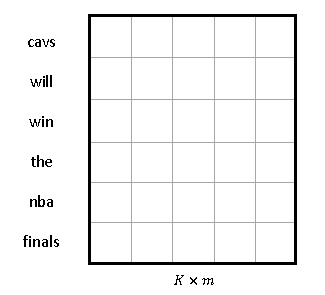
\includegraphics[width=0.55\textwidth]{sentenceMatrix}
  \caption{语句向量化的示意图}
  \label{fig:senVec}
\end{figure}

图\ref{fig:senVec}中每一行表示一个词语向量化得到的一个向量,所有行组成一个语句。在例子中,语句$\mathbf{s}=$\textit{cavs}$\oplus$\textit{will}$\oplus$\textit{win}$\oplus$\textit{the}$\oplus$\textit{NBA}$\oplus$\textit{finals}。语句$\mathbf{s}$中的每一个词语都将根据词向量模型转换成一个向量。这一步骤将语句$\mathbf{s}$转换成一个矩阵$\mathbf{B} \in \mathbb{R}^{Km}$,其中$K$为语句$\mathbf{s}$的长度,$m$为词向量模型设定的维度。对于任意一篇文档$\mathbf{d}_j$,我们能够将其文本摘要,即排序后的语句集合$\mathbf{S}_j = \left\{\mathbf{s}'_1, \mathbf{s}'_2, \cdots, \mathbf{s}'_k\right\}$转换成另一个矩阵$\mathbf{A}_j \in \mathbb{R}^{nm}$,其中$n$为文档长度的截断长度,即允许容纳的最大词语量。我们以图\ref{fig:docVec}为例进行说明。

\begin{figure}[!htbp]
  \centering
  % Requires \usepackage{graphicx}
  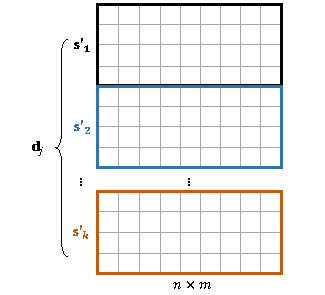
\includegraphics[width=0.65\textwidth]{documentMatrix}
  \caption{文档向量化的示意图}
  \label{fig:docVec}
\end{figure}

图\ref{fig:docVec}为词向量模型将一篇文档$\mathbf{d}_j$转换成矩阵$\mathbf{A}_j$的示意图。如果文档中的长度超过了阈值$n$,则进行截断;如果文档的长度不足$n$,则用零向量进行补全。本小节中的处理过程使得每一篇文档都能转换成一个固定大小的矩阵。但是,在截断或者补全零向量的操作会丢失部分信息或者引用无效的信息,这一问题还是有待今后的工作进行研究。

\subsection{卷积神经网络的训练}
\label{subsec3:cnnTraining}
在上一小节中,我们得到了表示文档的矩阵,我们将此当作输入来训练卷积神经网络。卷积神经网络的框架图如图\ref{fig:cnn}所示。

\begin{figure}[!htbp]
  \centering
  % Requires \usepackage{graphicx}
  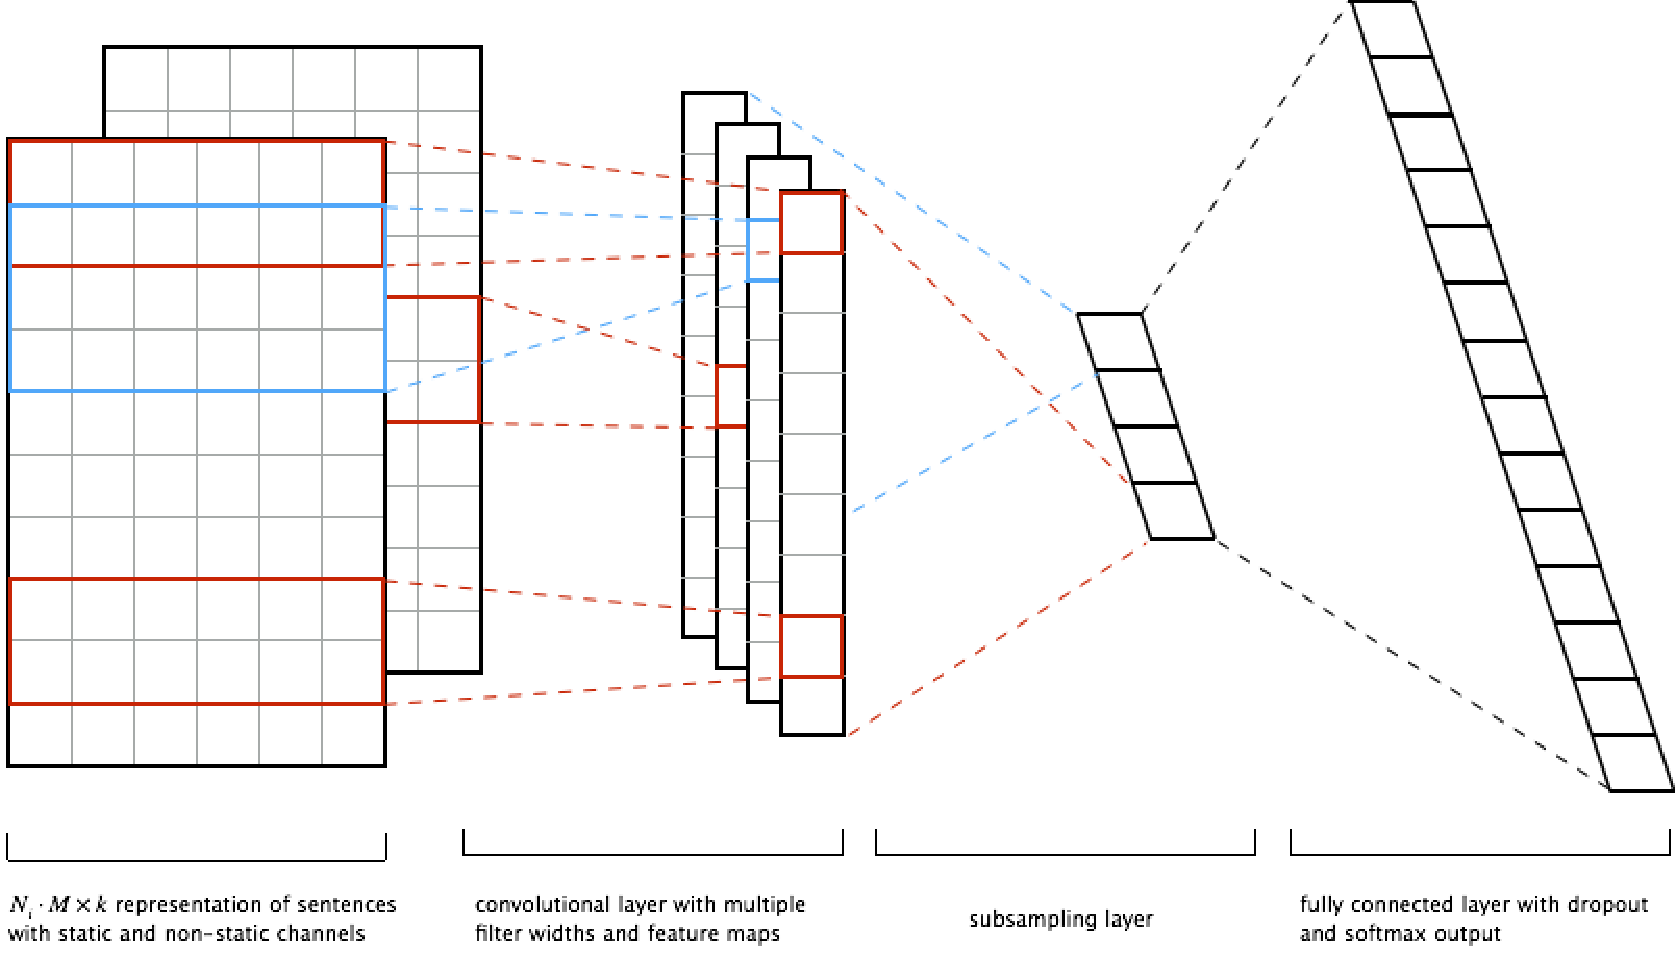
\includegraphics[width=0.85\textwidth]{cnn}
  \caption{三层卷积神经网络结构图}
  \label{fig:cnn}
\end{figure}

图\ref{fig:cnn}中的第一层为卷积层,包含多个宽度的滤波器。我们定义$\mathbf{w} \in \mathbb{R}^{hm}$为卷积层中的一个滤波器,其中$h$为滤波器的窗口大小,即一次性处理词语的窗口大小,$m$为滤波器的宽度,令其等于第\ref{subsec3:word2vec}小节中词向量模型设定的维度。该滤波器作用到一个窗口大小为$h$的文本上,文本中的词语表示成维度为$m$的向量。为了方便起见,我们使用$\mathbf{t}_{i:i+h}$来表示词语$\mathbf{t}_i, \mathbf{t}_{i+1}, \cdots, \mathbf{t}_{i+h}$的连接。一个滤波器$\mathbf{w}$作用到词语连接$\mathbf{t}_{i:i+h}$,将产生一个新的特征$c_i$,可表示成公式(\ref{eq:feature})所示,
\begin{equation}
\label{eq:feature}
	c_i=f(\mathbf{w} \otimes \mathbf{t}_{i:i+h} + b)
\end{equation}
其中$b \in \mathbb{R}$为偏置参数,$f$为一个非线性的函数,例如sigmoid函数等。值得注意的是,在本章中,我们令滤波器$\mathbf{w} \in \mathbb{R}^{hm}$的宽度等于词向量模型的维度。这个步骤与图像处理中的设置不同,这是由于设置一个宽度小于$m$的滤波器在文本处理中是没有意义的。文本中的词语被表示成$m$维的向量,因此截取其中的某些维度是无意义的。对于一篇文档,我们从上至下滑动滤波器,$\mathbf{w} \in \mathbb{R}^{hm}$将作用在不同的词语连接$(\mathbf{t}_{1:h}, \mathbf{t}_{2:h + 1}, \cdots, \mathbf{t}_{N - h + 1:N})$上,从而得到一个新的特征向量$\mathbf{c}$,其可表示为公式(\ref{eq:featureMap})所示,
\begin{equation}
\label{eq:featureMap}
	\mathbf{c}  = ({c_1},{c_2},...,{c_{N - h + 1}})^T
\end{equation}
其中$\mathbf{c} \in \mathbb{R}^{N-h+1}$。在经过卷积层后,得到的特征维数仍然很高,很容易出现过拟合的现象。为了解决这个问题,我们在卷积层后加上一个池化(Pooling)操作,也就是子采样(Subsampling),构成子采样层。子采样层能够大大降低特征的维数,避免过拟合。池化操作作用在特征向量$\mathbf{c}$,将得到$\mathbf{c}$中的最大值$c_{\max} = \max\limits_{c_i \in \mathbf{c}} c_i$。子采样层的目的是为了得到特征向量中最为重要的特征值,即具有最大的特征值。为了得到更多的特征值,我们可以调整窗口的大小来产生不同的特征向量。最后,子采样层得到的特征作为最后分类器的输入,该层为一个softmax函数的全连接层,输出层为文档在各个类别上的概率分布。

此外,我们使用了两个通道\upcite{kim2014convolutional}的词向量作为输入。其中一个通道在训练过程中保持不变,另一个通道通过反向传播进行微调。每一个滤波器都会作用于这两个通道来产生不同的特征。

\begin{algorithm}[!ht]
    \caption{\textit{VecCNN}($\mathbf{D}$)}\label{alg:cnn}
    \begin{algorithmic}[1]
    \REQUIRE $\mathbf{D}$
    \ENSURE \textit{CNN}
    \FOR{each $\mathbf{d}_j$ in $\mathbf{D}$}
        \FOR{each $t_i$ in $\mathbf{d}_j$}
            \STATE{${tf}_{ij} = \frac{p_{ij}}{\sum_{tl \in \mathbf{d}_j}{p_{lj}}}$}
            \STATE{${idf}_i = \log \frac{\vert \mathbf{D} \vert}{1 + \vert \{\mathbf{d} \in \mathbf{D} : \mathbf{t}_i \in \mathbf{d}\}\vert}$}
        \ENDFOR
    \ENDFOR
    \FOR{each $\mathbf{d}_j$ in $\mathbf{D}$}
        \FOR{each $\mathbf{s}_i$ in $\mathbf{d}_j$}
            \STATE{$I(\mathbf{s}_i, \mathbf{d}_j)=\frac{\sum \nolimits_{\mathbf{t}_i \in \mathbf{s}_i} {tf}_{ij}\cdot{idf}_i }{\log \left(\vert\mathbf{s}_i\vert\right)}$}
        \ENDFOR
        \STATE{$\mathbf{S}_j = \left\{\mathbf{s}'_1, \mathbf{s}'_2, \cdots, \mathbf{s}'_k\right\}$}
    \ENDFOR
    \FOR{each $\mathbf{S}_j$ in $\mathbf{D}$}
        \STATE{generate text matrix $\mathbf{A}_j$ based on $\mathbf{S}_j$}
    \ENDFOR
    \STATE{train \textit{CNN} based on the matrix set}
    \STATE {return \textit{CNN}}
    \end{algorithmic}
\end{algorithm}

本节中的算法步骤可以概括为算法\ref{alg:cnn}所示。如\textit{VecCNN}算法所示,输入为已标注的长文本信息集合,即文档集合$\mathbf{D}$,输出为所设计的卷积神经网络各层的参数。算法中的第1行至第6行为词语的tf-idf值计算。在这个步骤中,我们计算了每一个文档中各个词语的tf-idf值,为之后的文本摘要提取做准备。算法中的第7行至第12行,我们根据语句中词语的tf-idf值来对文档中的语句进行排序,从而挑选出关键语句代表文档的主题。这个过程减少了输入文本信息的规模,方便了之后卷积神经网络的训练。算法的第13行至第17行是卷积神经网络的训练。我们选择top-$k$的语句构建矩阵,作为卷积神经网络的输入,计算各个神经元中参数的梯度,通过迭代的方法求得极值,训练得到网络各层的参数。

\section{实验分析}
\label{sec3:experiment}
在本节中,我们进行了几组实验来验证所提出的方法。首先,我们介绍本节中实验所使用的实验数据集以及实验设置。然后,我们将展示实验结果并详细地分析实验结果。本节中所有的实验都在4 CPU、32 GB内存的服务器运行,操作系统为Ubuntu 14.04 x64。文章的算法基于Python实现,在python 3.4的环境下运行。

\subsection{实验设置}
\label{subsec3:settings}
为了验证与评估我们所提出的算法,我们使用不同领域和量级大小的数据集来进行实验。其中20 newsgroups文本数据集(\textit{newsgroups}\footnote{\url{http://scikit-learn.org/stable/datasets/twenty_newsgroups.html}})包含大约18,000篇20个主题的新闻报道。数据集分成两个子类,一类用于训练,一类用于实验测试。其中Large Movie Review数据集\upcite{maas2011learning}(\textit{LMR}\footnote{\url{http://ai.stanford.edu/~amaas/data/sentiment/}})为大电影评论的数据集,为二元的情感分类数据集。其中包含约25,000篇情感鲜明的评论用于训练,还有25,000篇评论用于训练。Li等人\upcite{li2002learning}提供了一个问题分类的实验数据集(\textit{QC}\footnote{\url{http://cogcomp.cs.illinois.edu/Data/QA/QC/}})。数据集包括5个训练集以及一个TREC中的真实测试集。数据集的一个简要说明如表\ref{tab:datasetCNN}所示。

\begin{table}
    \centering
    \caption{数据集特性}\label{tab:datasetCNN}
    \begin{tabular}{ccc}
        \hline
         & \textit{size} & \textit{label}\\
        \hline
        \textit{newsgroups} & 18000 & 20\\
        \hline
        \textit{LMR} & 50000 & 2\\
        \hline
        \textit{QC} & 15500 & 6\\
        \hline
    \end{tabular}
\end{table}

在算法的比较方面,我们将所提出的\textit{VecCNN}算法与两个基准算法朴素贝叶斯(\textit{Naive Bayes})和支撑向量机(\textit{Support Vector Machine})进行比较。我们选取了几个评判准则来评估算法的性能,包括准确率、召回率、$F_1$值。为了测试\textit{VecCNN}算法的可扩展性,我们在不同量级大小的数据集中进行实验,记录其运行时间。此外,实验中,词向量模型的维度设置为$m=200$,文档长度的截断阈值设置为$n=300$。

\subsection{结果分析}
\label{subsec3:analysis}
为了验证算法的准确性,我们在数据集\textit{newsgroups}、\textit{LMR}和\textit{QC}上运行了朴素贝叶斯算法、支撑向量机算法以及\textit{VecCNN}算法,进行对比分析。对于每一个数据集,实验运行算法5次,取平均值作为最后的结果。准确率的实验结果如表\ref{tab:avgPrecision}所示。

\begin{table}[!ht]
    \centering
    \caption{算法在各数据集上的平均准确率}\label{tab:avgPrecision}
    \begin{tabular}{cccc}
        \hline
         & \textit{newsgroups} & \textit{LMR} & \textit{QC} \\
        \hline
        \textit{Bayes} & 0.36 & 0.66 & 0.51\\
        \hline
        \textit{SVM} & 0.47 & 0.80 & 0.52\\
        \hline
        \textit{VecCNN} & \textbf{0.72} & \textbf{0.88} & \textbf{0.99}\\
        \hline
    \end{tabular}
\end{table}

从表\ref{tab:avgPrecision}可以看出\textit{VecCNN}算法与朴素贝叶斯算法、支撑向量机算法相比,在\textit{newsgroups}数据集上的分类准确率相对较高。在\textit{LMR}数据集上,\textit{VecCNN}算法与支撑向量机算法的准确率相近,而朴素贝叶斯算法准确率较低。在\textit{QC}数据集上,\textit{VecCNN}算法的准确率远好于其余两个算法。由此可以看出,在多元分类问题中,\textit{VecCNN}相对其他两种算法准确率更高,而在二元分类问题中,\textit{VecCNN}与支撑向量机算法的准确率相近。表\ref{tab:avgRecall}为各个算法在数据集上的召回率结果,表\ref{tab:avgF1}为各个算法在数据集上的$F_1$值结果。结果都显示了\textit{VecCNN}算法的性能。

\begin{table}[!ht]
    \centering
    \caption{算法在各数据集上的平均召回率}\label{tab:avgRecall}
    \begin{tabular}{cccc}
        \hline
         & \textit{newsgroups} & \textit{LMR} & \textit{QC} \\
        \hline
        \textit{Bayes} & 0.18 & 0.66 & 0.51\\
        \hline
        \textit{SVM} & 0.46 & 0.80 & 0.52\\
        \hline
        \textit{VecCNN} & \textbf{0.69} & \textbf{0.93} & \textbf{0.99}\\
        \hline
    \end{tabular}
\end{table}

\begin{table}[!ht]
    \centering
    \caption{算法在各数据集上的平均$F_1$值}\label{tab:avgF1}
    \begin{tabular}{cccc}
        \hline
         & \textit{newsgroups} & \textit{LMR} & \textit{QC} \\
        \hline
        \textit{Bayes} & 0.18 & 0.66 & 0.51\\
        \hline
        \textit{SVM} & 0.45 & 0.80 & 0.51\\
        \hline
        \textit{VecCNN} & \textbf{0.70} & \textbf{0.88} & \textbf{0.99}\\
        \hline
    \end{tabular}
\end{table}

对于\textit{LMR}数据集,我们计算了各个算法的roc曲线,如图\ref{fig:roc}所示。图中的roc曲线描述了各个算法训练出的二元分类器在判别阈值变化时,性能的变化。曲线下的面积越大说明算法的性能越好。

\begin{figure}[!htbp]
  \centering
  % Requires \usepackage{graphicx}
  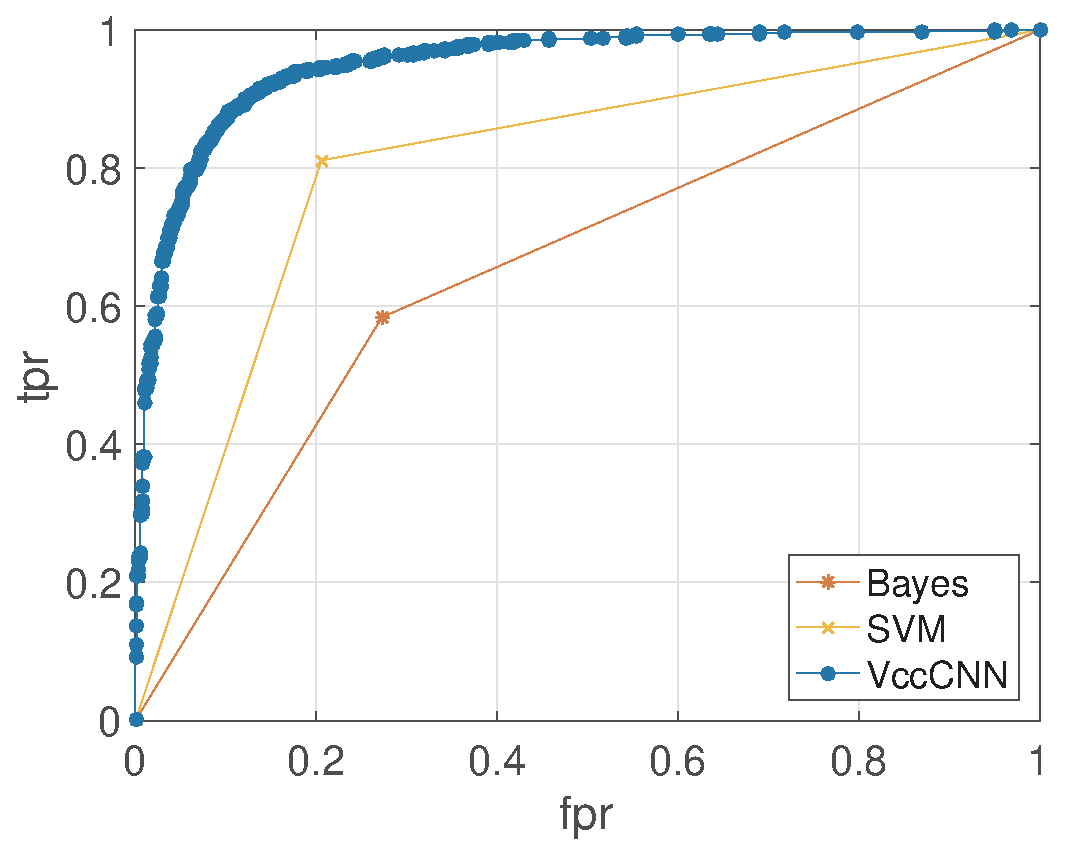
\includegraphics[width=0.55\textwidth]{roc}
  \caption{算法在\textit{LMR}数据集上的roc曲线}
  \label{fig:roc}
\end{figure}

图\ref{fig:roc}的横坐标\textit{fpr}为假阳性率(false positive rate),表示被预测为正样本的负样本比例;纵坐标\textit{tpr}为真阳性率(true positive rate),表示被预测为正样本的正样本比例。由图可以看出,\textit{VecCNN}算法的roc曲线下面积相对较大,说明\textit{VecCNN}算法相对于其他两个算法更加的有效。

\textit{newsgroups}和\textit{QC}数据集为多标签数据集,我们给出了算法在各个类别的准确率和召回率,如图\ref{fig:barNGP}至\ref{fig:barQCR}所示。

\begin{figure}[!htbp]
   \begin{minipage}{0.48\textwidth}
     \centering
     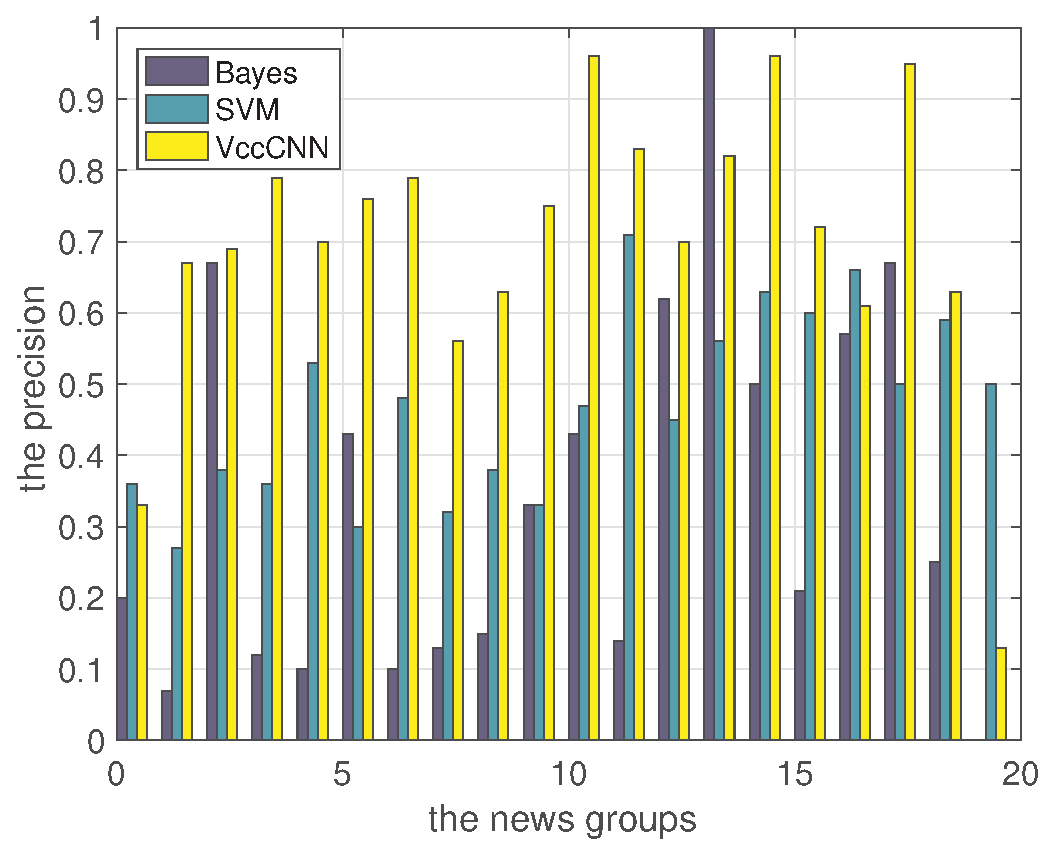
\includegraphics[width=\linewidth]{barNGP}
     \caption{算法在\textit{newsgroups}数据集上各类别的准确率}
     \label{fig:barNGP}
   \end{minipage}
   \hfill
   \begin{minipage}{0.48\textwidth}
     \centering
     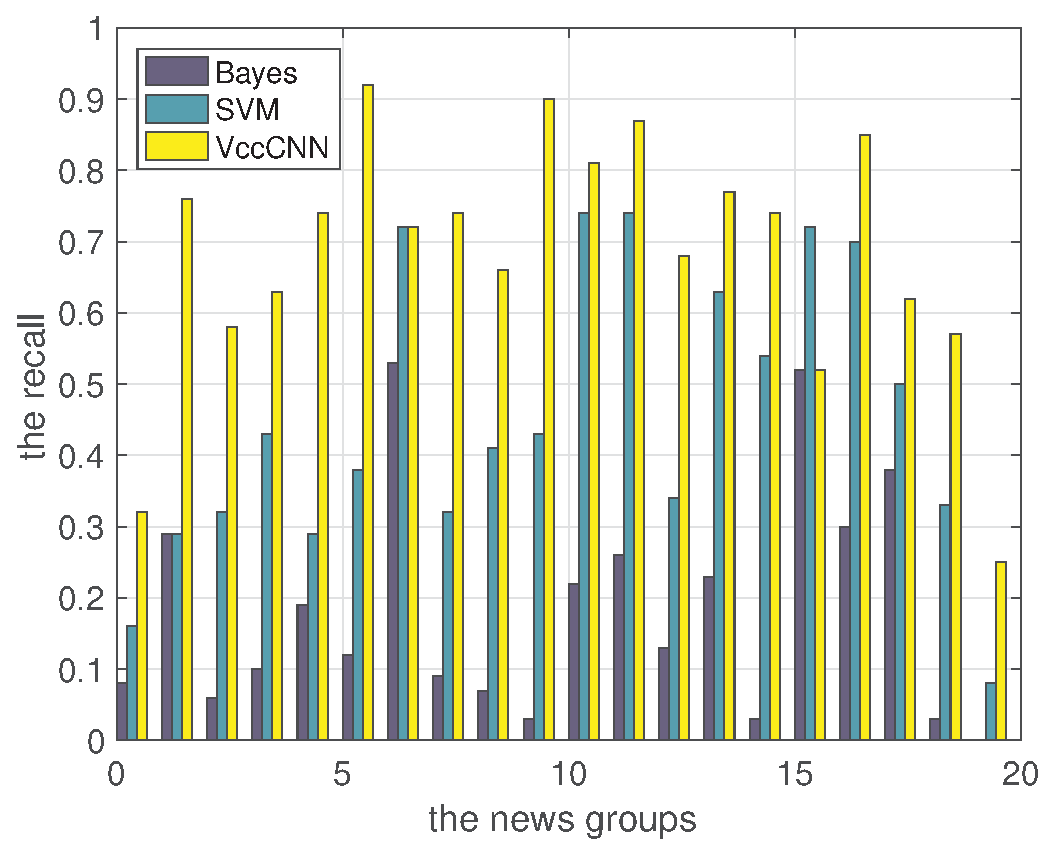
\includegraphics[width=\linewidth]{barNGR}
     \caption{算法在\textit{newsgroups}数据集上各类别的召回率}
     \label{fig:barNGR}
   \end{minipage}
   \\ 
   \begin {minipage}{0.48\textwidth}
     \centering
     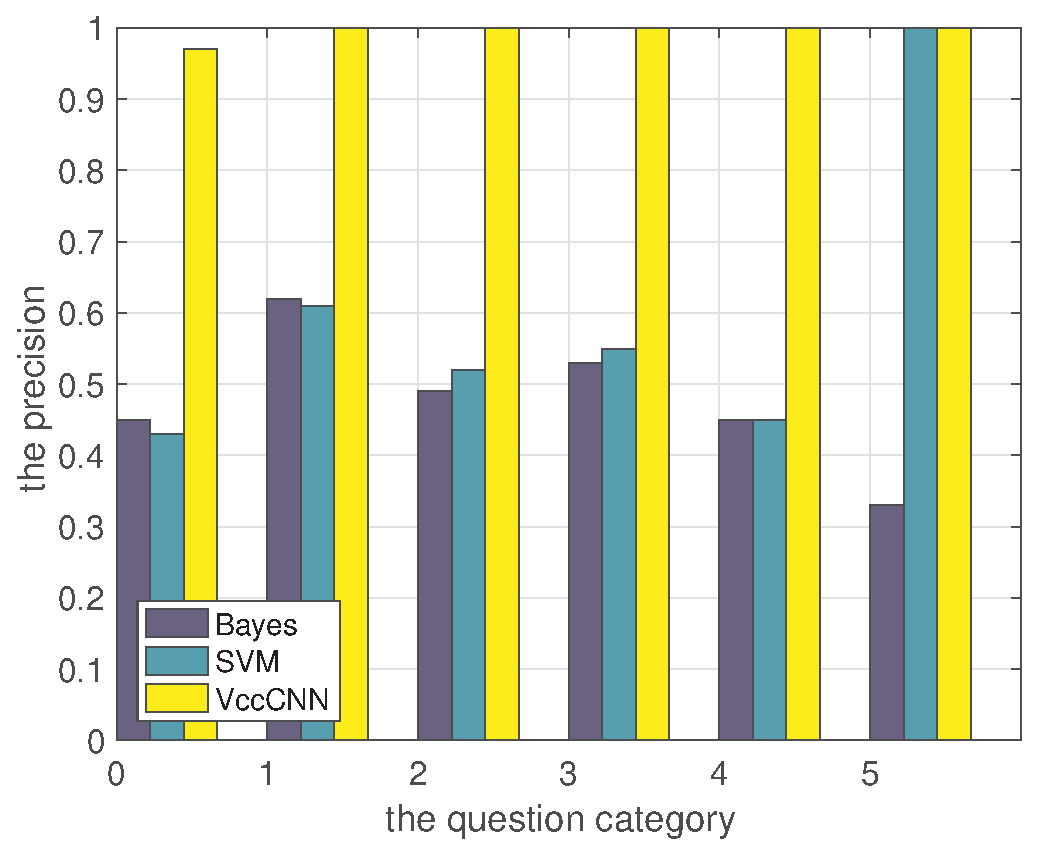
\includegraphics[width=\linewidth]{barQCP}
     \caption{算法在\textit{QC}数据集上各类别的准确率}
     \label{fig:barQCP}
   \end{minipage}
   \hfill
   \begin {minipage}{0.48\textwidth}
     \centering
     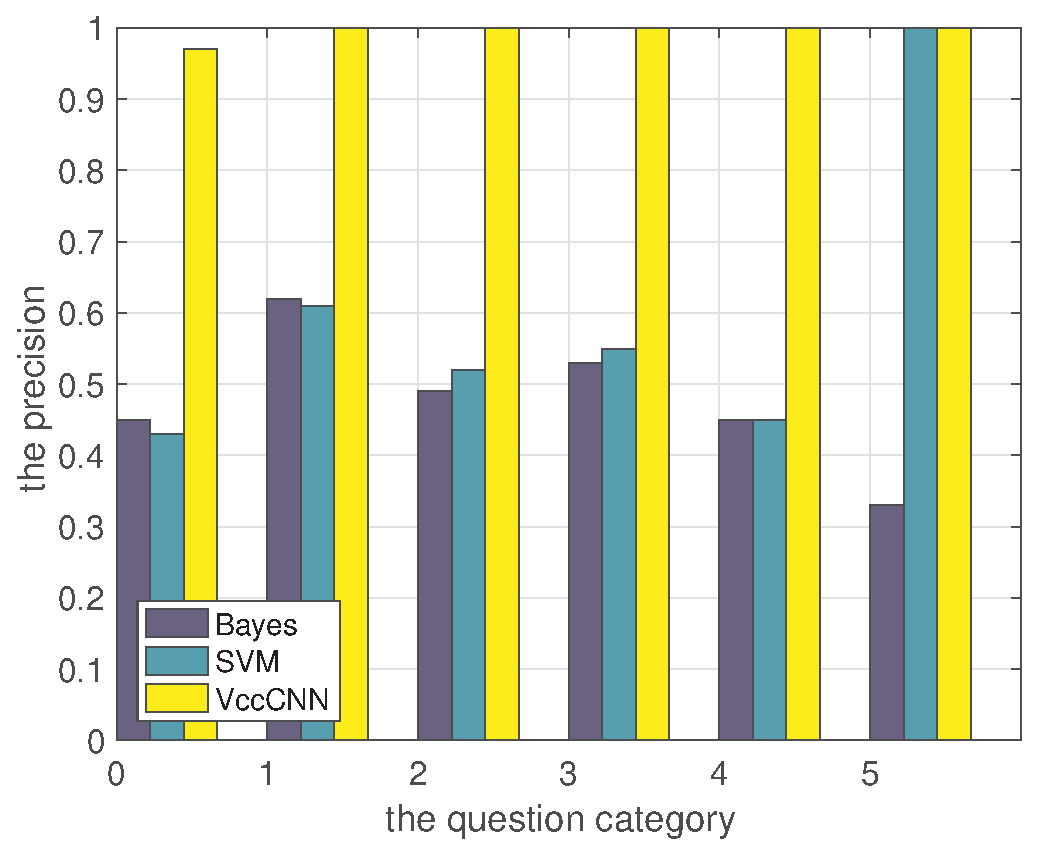
\includegraphics[width=\linewidth]{barQCR}
     \caption{算法在\textit{QC}数据集上各类别的召回率}
     \label{fig:barQCR}
   \end{minipage}
\end{figure}

如图\ref{fig:barNGP}所示,\textit{VecCNN}算法的准确率在绝大多数类别中要优于支撑向量机算法,在所有的类别中都比朴素贝叶斯算法要好高。图\ref{fig:barNGR}表示,在绝大多数类别中,\textit{VecCNN}算法的召回率都要优于其他两种算法。图\ref{fig:barQCP}显示了在\textit{QC}数据集各类型的问题分类中,\textit{VecCNN}算法准确率相对于其他两种算法更高。图\ref{fig:barQCR}显示了\textit{VecCNN}算法在\textit{QC}数据集上各类别的召回率更高。由以上的实验,我们验证了所提出算法的有效性,\textit{VecCNN}算法在多元分类问题上相对于另外两种基准算法性能更好,在二元分类问题上同样也有效。

为了验证\textit{VecCNN}算法的可扩展性,我们使用不同规模的数据集来运行实验,记录其运行时间。对于数据集,我们均匀随机地选取指定大小规模的子集,运行算法5次,计算其平均运行时间作为最终结果。实验结果如图\ref{fig:scalabilityCNN}所示。

\begin{figure}[!htbp]
    \centering
    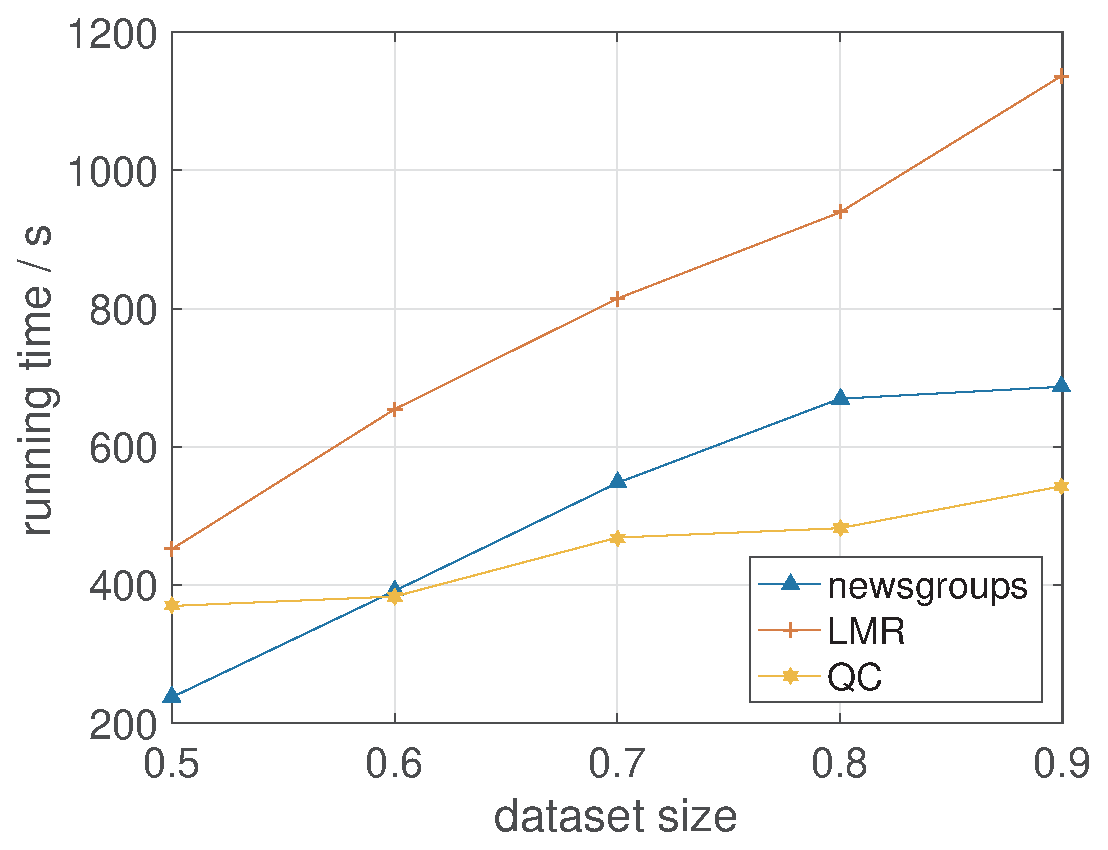
\includegraphics[width=0.55\textwidth]{scalability}
    \caption{算法的可扩展性}
    \label{fig:scalabilityCNN}
\end{figure}

图\ref{fig:scalability}中横坐标为数据集相对于原始数据集的比例,纵坐标为训练网络的运行时间。我们可以看出,运行时间的增长是近似线性的,因此所提出的算法具备可扩展性。
\section{本章小结}
\label{sec3:conclusion}
本章提出了一个结合文本摘要提取、词向量模型以及卷积神经网络的长文本信息分类算法。首先,算法通过文本中词语的tf-idf值来对关键语句进行排序,提取文本核心语句,得到文本摘要。然后,所得到的文本摘要通过词向量模型转换为向量形式。最后,文本转换成的向量作为神经网络的输入用于训练网络参数,从而得到分类器。其中,算法提出了一种基于词语tf-idf值的语句排序方法,能够快速的提取文本的摘要。同时,算法将词向量模型与卷积神经网络结合来实现文本分类。实验验证了所提出算法的正确性和有效性,在多个评判准则中,所提出的算法都优于基准算法。

下一步工作中,训练更加准确的词向量模型以及根据不同的数据调整神经网络的结构是提高文本分类性能的途径。
\chapter{基于概率阅读的事件传播模型研究}
\label{chap5:main}
信息传播的\textbf{信息传播模型}分析是社交网络分析中的一个重要研究点,网络热点事件通过社交网络平台迅速传播、发酵,从而在短时间内形成信息爆发、造成极大的影响。社交网络加速了新闻、通知等信息的传播,使得人们接受信息的速率加快,传播信息的成本降低,在一定程度上方便了人们的生活。但是,在社交网络中,人人都可以是信息的生产者、传播者和接收者,每一个社交网络用户都能通过平台发布传播信息。在社交网络中制造舆论热点,进行信息传播的代价相对于传统媒体较低,因此很容易被不法分子利用,对社会安全以及人身财产等造成损失。已有的信息传播模型研究主要包括独立级联模型和线性阈值模型等,这些模型对信息的传播进行了量化,对信息的传播范围进行了传播范围的评估。但是,仍然有一些需求在实际应用中得不到满足。

在信息传播过程中,一个被激活的节点(信息接收者)将尝试继续传播该信息,去激活下一个节点,从而产生级联效应。在实际应用中,一个事件往往由多条主要的信息组成,因此一个事件的传播将由多个传播网络组合而成。所以事件的传播模型首先需要考虑的是多个传播网络的融合问题。其次,社交网络中存在很多的垃圾用户,这些用户活跃度低,或者是由水军控制,会影响到影响力量化的计算,因此需要建立垃圾用户过滤的机制,除去这些干扰噪声。最后,信息的叶子节点,即事件传播的最终的接收者(不再进行下一轮传播)是否阅读到了该信息是概率性的,因此根据用户的社交行为来为用户阅读信息进行建模能够提高影响力量化的准确度。出于精确量化事件传播的影响力的需求,本章提出了一个基于概率阅读的事件传播模型,将多信息传播网络融合、垃圾用户过滤和概率阅读模型综合考虑,为事件在社交网络中的传播进行建模,精确量化事件的传播影响力。

本章的主要工作可以总结如下。首先,基于事件中单条信息的传播网络,我们对多个传播网络进行融合,去除掉重复的节点。其次,利用用户在社交网络中的社交属性,基于逻辑回归模型进行建模,使用梯度下降法进行参数训练,最终得到模型用于垃圾用户过滤。然后,利用用户在社交网络中的时间线上的社交属性,对用户阅读到信息的概率进行建模,对概率阅读模型进行参数训练,得到的模型最终用来预测用户阅读到信息的概率。最后,本章对提出的模型进行了验证,实验使用新浪微博的真实数据集,实验结果证明了模型的有效性。

本章的内容组织如下:第\ref{sec5:motivation}节介绍本章的研究动机,讨论了传统的传播模型的不足之处以及研究基于概率阅读的事件传播模型的意义。第\ref{sec5:definition}节介绍了相关的定义,对本章中所研究的问题进行了定义。第\ref{sec5:method}节介绍了方法描述,详细地阐述了本章提出的模型以及建立过程。第\ref{sec5:experiment}节进行了实验分析,通过实验结果验证了模型的正确性,并对实验结果进行了分析。最后,第\ref{sec5:conclusion}节对本章进行了总结。
\section{研究动机}
\label{sec5:motivation}
在Web 2.0时代,社交网络媒介逐渐开始取代如同报刊、杂志、新闻等传统媒介,占据了信息传播的主导位置。随着各大社交网站的发展,如国外的脸书(Facebook)、推特(Twitter)等,国内的新浪微博、腾讯微博等。与此同时,传统媒介也开始结合社交网络媒介,纷纷开设自己的公共主页,通过互联网及时发布信息,将信息在第一时间推送给用户。在不如大数据时代后,各大社交网络门户的用户呈现几何式爆炸增长的趋势,一条信息通过网络平台在短时间内能够传播影响到的数以百万计的用户。相比于传统媒介,社交网络媒介在信息传播过程中的传播效率与传播范围都大大增强,然而一些虚假信息通过社交网络媒介的传播也能在短时间内迅速扩散,从而可能造成社会的恐慌、用户财产的损失等问题。因此,在大数据时代,社交网络媒介中的信息传播问题成为了信息安全领域的一个研究热点。

信息传播模型定义了社交网络中影响力传播的方式和机制,是研究社交网络中事件传播影响的基础。已有的研究对传播模型做出了深入的研究,其中广泛应用的模型主要有\textbf{独立级联模型}(\textit{Independent Cascade Model})\upcite{goldenberg2001talk,Goldenberg2001Using}和\textbf{线性阈值模型}(\textit{Linear Threshold Model})\upcite{Granovetter1986Threshold,granovetter1983threshold},这两种模型分别从不同的角度描述了信息传播的过程。

独立级联模型是一种概率传播模型,源于市场营销模型研究。独立级联模型基于概率,每一个传播节点在自身转变为活跃状态后,都可以以一定的概率取激活其后继节点,并且多个活跃节点试图影响同一个邻居节点的事件是独立的,所以称之为独立级联模型。独立级联模型是一种比较经典的模型,适用范围广,能够诠释大多数情况的信息传播过程。

线性阈值模型主要源于节点的特异性研究,模型核心出发点为节点的激活阈值,多个活跃节点试图影响同一后继节点的过程是非独立的,节点激活的成功与否取决于多个节点的加权影响是否超过后继节点的阈值。线性阈值模型体现了信息传播过程中影响的累积效应特性,即节点对后继节点的影响是多个节点的累积。

除了上述的信息传播模型外,目前还有一些其他的信息传播模型研究。最为简单的模型是\textbf{统一模型}(\textit{Uniform Model}),模型假设所有节点的传播影响概率都是一个常数,例如0.01。该模型不考虑节点之间的关系,即边的关系。所有的节点对其邻居节点的影响是相同的,不根据结构的变化而变化。此外,模型还假设一个节点对于其所有的邻居节点的影响也是相同的,即不区分邻居节点之间的差别。很显然,这两个假设在实际应用中都是不能得到满足的。基于统一模型的改进为\textbf{三态模型}(\textit{Trivalency Model}),该模型对统一模型中的第一个假设进行了修正。三态模型不再假设所有的节点的传播影响概率是相同的,节点的传播影响概率是均匀随机地从预先设置的概率集合中选取,例如$\{0.001,0.01,0.1\}$。在统一模型中,每一个节点的传播影响概率是相同的,不可区分的。而在三态模型中,节点的传播影响概率是不同的,是可区分的。三态模型的核心思想是将节点的传播影响概率进行了区分,例如传播影响概率为0.001的节点对应于低影响力的节点,传播影响概率为0.01的节点对应于中影响力的节点,传播影响概率为0.1的节点对应于高影响力的节点。在统一模型和三态模型中,节点的传播影响概率都与网络的结构不相关。在\textbf{加权独立级联模型}(\textit{Weighted Independent Cascade})中,传播影响概率与网络的边相关,即与用户关系相关。传播影响概率定义为$p_{u,v}=1 / d_{in}\left(v\right)$,其中$d_{in}\left(v\right)$为节点$v$的入度。该模型相比于上述的两种模型能够更好地诠释信息在社交网络中的传播过程,对于网络中的节点进行了深层次的区分。入度小的节点受到每个入读邻居节点的影响要大于入度大的节点受到的影响,传播影响概率不是简单地从一个常数集合中选取,而是与网络结构相关。另一方面,节点对于其出度邻居节点的传播影响概率不一定是相同的,这是由于出度邻居节点的入度不同。尽管加权独立级联模型拥有以上良好的特性,然而模型的传播影响概率的计算方法仍然缺乏理论保证,传播影响概率与网络的结构相关,但是没有考虑节点之间的历史传播影响概率。\textbf{选举模型}(\textit{Voter Model})\upcite{evendar2011a}是一种广泛应用在统计物理和粒子系统中的一种模型。在选举模型中,各节点随机选取其某一个前驱节点的状态作为自己的状态。上述的各种模型都对信息传播过程的特点进行了研究和建模,为传播分析提供了理论依据,奠定了研究基础。

在社交网络中,独立级联模型最为适应于社交网络的特性。以微博为例,信息的发布源为某个用户,称之为博主。博主发布的博文将推送至博主所有的粉丝,而粉丝接收到此信息后,将以一定的概率转化为激活状态(即转发此条博文)。如果粉丝转发了博文,则其粉丝又会接收到该信息,进而产生级联效应,促使更多的用户接收到该信息。

社交网络具有自身的特性,特别是进入大数据时代后,平台中的信息量庞大。网络中的节点接收到前驱节点信息的概率与该节点所有的前驱节点的状态有关。以微博为例,用户是否能够接收到其关注用户的信息取决于用户在信息推送时是否处于在线状态,即用户接收信息的概率与信息推送时间和用户在线时间的间隔有关。同时在社交网络中,一些节点的活跃度低,为无效节点,不能将其统计入全局的影响传播中。例如,微博中存在很多的垃圾用户,在计算事件的传播影响力时,需要将其滤出才能还原真实的信息传播过程。传统的信息传播分析主要针对单条博文,而在实际应用中,微博中的一个热点事件往往由多条博文组成。因此,对于事件进行传播分析需要针对多个博文进行分析,对应于信息传播过程中多个信息源的热点。同时,用户阅读到信息的概率与信息的发布时间和接收用户的在线时间的间隔相关,需要建立阅读模型来模拟信息传播过程中特性。本章将针对传统的信息传播模型中存在的不足以及在实际应用中的缺陷,结合多源传播网络融合、垃圾用户过滤和概率阅读模型来进行事件的传播分析。
\section{相关定义}
\label{sec5:definition}
在本小节中,我们对所研究的问题进行详细的描述,并对涉及到的概念进行定义和解释。
\subsection{社交网络的基本定义}
\label{subsec5:socialNetwork}
社交网络是由社会个体成员以及社会个体成员之间的联系组成的一种复杂的关系网络。在相关的社交网络研究中,社交网络通常用图$\mathcal{G}=\left(\mathcal{V},\mathcal{E},\mathcal{W}\right)$来表示。其中节点集合$\mathcal{V}=\{v_1,v_2,\cdots,v_n\}$表示社交网络中的社会个体成员,$n$表示整个网络中个体成员的数目。各个社会个体成员之间的关系由图$\mathcal{G}$的边的集合表示,即$\mathcal{E} \subseteq \mathcal{V} \times \mathcal{V}$,其中$\mathcal{V} \times \mathcal{V}$表示节点的笛卡尔集。社会个体成员之间的关系可以是价值观、合作、关联、亲属、好友等各种类型的关系。社会个体的权重以$\mathcal{W}=\{w_1,w_2,\cdots,w_n\}$来表示,用于表示社会个体成员的重要性,例如影响力、公信力等等特征。

\begin{figure}[!ht]
    \centering
    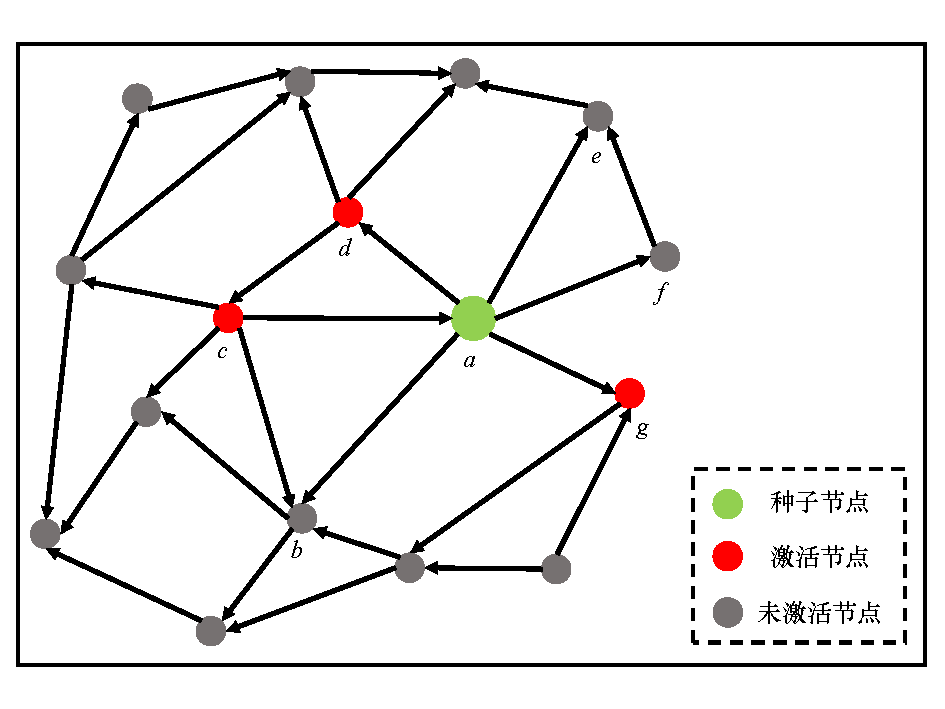
\includegraphics[width=0.8\textwidth]{infoSocial}
    \caption{社交网络中信息传播示意图}
    \label{fig:infoSocial}
\end{figure}

图\ref{fig:infoSocial}给出了社交网络的结构以及信息传播的示意图。信息传播过程可以形式化地描述如下,社交网络中的节点存在两种状态,激活与未激活。在独立级联模型下,给定种子节点后,种子节点首先被激活,然后会以一定概率去激活其他节点,进而形成级联效应。即当节点$u$被激活后,状态由未激活转变成激活,然后节点$u$会以一定的概率去激活处于未激活状态下的邻居节点。如若激活成功,则邻居节点将由未激活状态转变为激活状态,并具备传播能力。如图\ref{fig:infoSocial}中所示,节点$a$为种子节点,在信息传播一开始时被激活,节点$a$在被激活后将以一定的概率去激活其邻居节点$b$、$d$、$e$、$f$、$g$。假设传播情况如图中所示,节点$c$、$d$、$g$被激活,节点$e$、$f$未被激活。由为激活状态转变成激活状态这一过程是不可逆的,这种由未激活状态转变成激活状态的过程称之为信息传播过程。

在社交网络中用户之间的关系主要分为两种,有向关系与无向关系。有向关系表示节点与节点之间的关系是有向的,例如新浪微博、推特中的关注关系。无向关系表示节点与节点之间的关系是无向的,例如脸书中的好友关系。二者的不同之处在于有向图中节点与节点的关系是单向的,可以用有向图表示。而无向关系中节点与节点之间的关系是双向的,可以用无向图表示。特别地,无向关系可以用双向的有向关系来表示。例如,如果节点$u$关注节点$v$,但是节点$v$不一定关注节点$u$。如果节点$u$与节点$v$是好友关系,则节点$v$与节点$u$也是好友。在社交网络中,这两种关系都普遍出现,可以用不同的图结构来表示。

\subsection{独立级联模型}
\label{subsec5:icModel}
Gruhl等人\upcite{gruhl2004information}首先信息传播模型的传播概率的学习进行了研究,Saito等人\upcite{saito2008prediction}研究了独立级联模型下的信息传播概率。独立级联模型中各个节点之间的影响是相互独立的,每个节点成为激活节点后都有一定的概率来激活其邻居节点。多个节点对同一个节点的激活是相互独立的。

在给定一个初始种子节点集合$S$后,在独立级联模型下信息传播的过程如下所示。在时刻$t=0$,社交网络中节点仅有集合$S$中的节点被激活,其余的节点为非激活状态。如果节点$u$在在时刻$t$被激活,则节点$u$由未激活状态转变成激活状态。在$t+1$时刻,节点$u$将有能力激活其后继节点。假设节点$u$存在一个后继节点$v$,令节点$u$激活节点$v$的概率为$p_{u,v}$。如果节点$u$在$t+1$时刻成功激活节点$v$,则节点$v$由未激活状态变成激活状态,在$t+2$时刻,节点$v$将有能力去激活其后继节点。如果节点$v$未被激活,则会保持未激活状态,但是节点$v$可能在未来的时刻由其他的前继节点激活。信息传播过程将持续到没有节点被激活的时刻为止。

假设$\mathcal{G}=\left(\mathcal{V},\mathcal{E}\right)$为一个社交网络。定义\textbf{信息传播时序}(\textit{information diffusion episode})为一个时间序列$\langle D\left(0\right), D\left(1\right), \cdots, D\left(T\right) \rangle$,且满足条件$D\left(i\right) \cap D\left(j\right) = \emptyset$。其中$T$代表着整个信息传播过程的持续时间,$D\left(t\right)$表示在时间$t$时刻被激活的节点集合。$D\left(0\right)$表示在时间$t=0$时刻被激活的节点,即初始的种子节点集合。约束$D\left(i\right) \cap D\left(j\right) = \emptyset$保证了已经激活的节点不会再变成未激活状态。信息传播过程将持续到$T$时刻结束,其中$D\left(T\right) = \emptyset$,即没有新的节点被激活时,信息传播过程结束。

\begin{figure}[!ht]
    \centering
    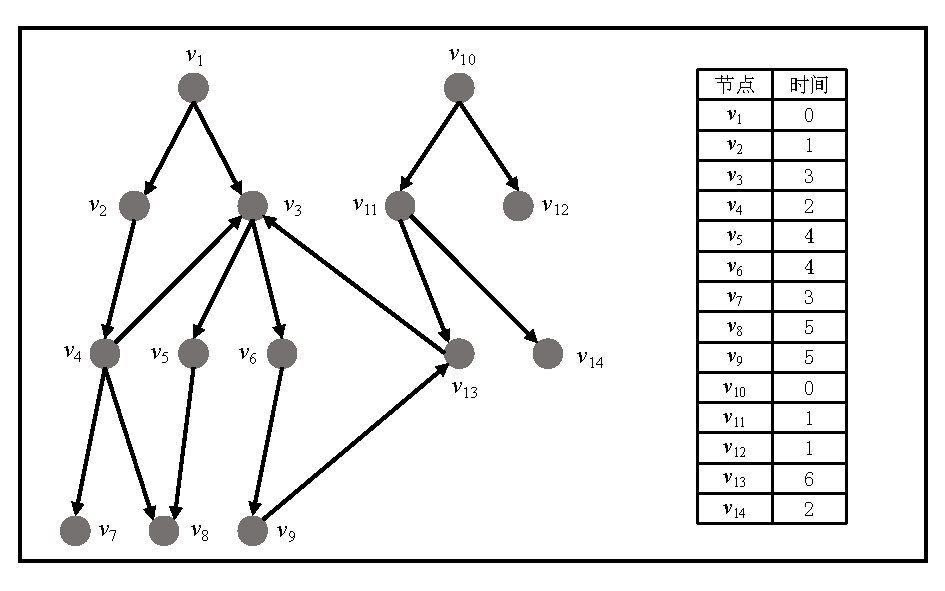
\includegraphics[width=1\textwidth]{infoDiffIC}
    \caption{独立级联模型下信息传播过程示意图}
    \label{fig:infoDiffIC}
\end{figure}

图\ref{fig:infoDiffIC}给出了一个独立级联模型下的信息传播过程的例子。节点$v_1$与节点$v_{10}$为种子节点,故$D\left(0\right)=\{v_1,v_{10}\}$。下一时刻,节点$v_1$激活节点$v_2$,节点$v_{10}$激活节点$v_{11}$和节点$v_{12}$,因此$D\left(1\right)=\{v_2,v_{11},v_{12}\}$。因为$D\left(1\right) \neq \emptyset$,所以信息传播继续进行。按照传播的规则,在$t=2$时刻,$D\left(1\right)$中的节点将有概率激活其后继节点,因此$D\left(2\right)=\{v_4,v_{14}\}$。在$t=3$时刻$D\left(3\right)=\{v_3,v_7\}$,在$t=4$时刻$D\left(4\right)=\{v_5,v_6\}$,在$t=5$时刻,$D\left(5\right)=\{v_8,v_9\}$,在$t=6$时刻,$D\left(6\right)=\{v_{14}\}$。而在$t=7$时刻,$D\left(7\right)=\emptyset$,信息传播过程结束。

\subsection{事件的传播}
\label{subsec5:affair}
基于社交网络的定义以及独立级联模型,我们以新浪微博为例,对社交网络中的事件传播进行研究分析。社交网络中的事件是指在特定的时间区间内,对某一个热点事件进行套路的博文集合。信息通过初始的几个信息源引发更多的人参与讨论和传播,从而影响到更多的社会个体。我们对微博中的事件作形式化的定义,如定义所示。

\begin{mydef}[事件]
\label{def:event}
社交网络中的事件是在一个时段内对同一个主题的信息的集合,与时间和内容相关。令$A$表示事件,则$A=\{a_1, a_2, \cdots, a_n\}$,其中$a_i$为讨论事件$A$的一条信息,由某一个用户发布,而事件$A$中的多条信息可能由同一个人发布。
\end{mydef}

在新浪微博中,事件在用户间主要通过阅读行为、评论行为、转发行为等进行传播,这三种行为对于事件传播的影响力贡献有所区别。
\begin{itemize}
  \item \textbf{阅读行为},指用户阅读到了其时间线上的信息,但是没有做出任何相应的相应行为。时间线上的信息有一定概率被用户所阅读到,这个概率与信息发布时间和用户的活跃时间的间隔相关。因此,阅读行为对于事件传播影响力的贡献是概率性的。
  \item \textbf{评论行为},指用户在阅读到其时间线上的信息后,对信息进行了评论,可以看作是一种特殊的阅读行为,即阅读到该信息的概率为1。因此,评论行为对于事件传播影响力的贡献是确定性的,但是信息的传播在该节点终止,不能产生进一步的传播,即不能产生级联效应。
  \item \textbf{转发行为},指用户阅读到时间线上的信息后,对信息进行了转发,即自身也变成了一个传播源。转发行为不仅对于事件传播影响力的贡献是确定性的,而且转发信息的用户自身也具备了传播能力,产生了级联效应。
\end{itemize}

由上可以看出不同的行为对于事件的传播影响的贡献是不同的,针对不同的用户的行为,需要按照不同的计算方式来衡量其对于事件传播影响力的贡献。在独立级联模型下事件的初始种子节点集合为发布事件中信息的用户集合。令发布事件中信息的用户集合为$S=\{s_1,s_2,\cdots,s_m\}$,其中$s_i$为某个用户,则初始种子节点集合为$S$。在信息传播过程中,转发信息的用户在转发行为的时刻转变为激活节点,具备传播信息的能力,即可能激活其他的用户变为激活状态,形成级联效应。

\begin{figure}[!ht]
    \centering
    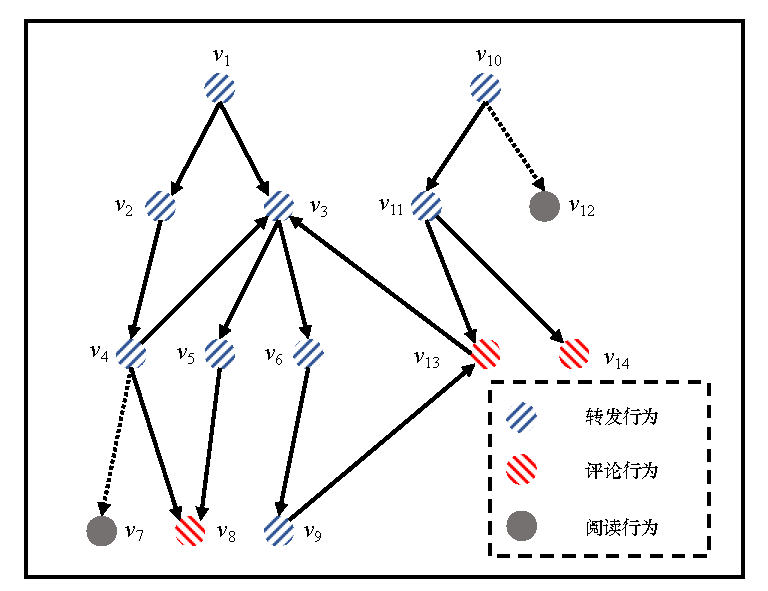
\includegraphics[width=0.9\textwidth]{affairInf}
    \caption{不同行为对于事件传播影响力的贡献}
    \label{fig:affairInf}
\end{figure}

如图\ref{fig:affairInf}所示,图中为三种行为在事件的传播中对影响力的贡献示意图。例如节点$v_4$转发了节点$v_2$发布的信息,则节点$v_4$对于事件传播影响力的贡献是确定性的,并且节点$v_4$具备了传播信息的能力。节点$v_7$以一定的概率阅读了节点$v_4$发布的信息,故$v_7$对于事件的传播影响力贡献是概率性的。节点$v_8$评论了节点$v_4$发布的信息,故$v_8$对于事件的传播影响力贡献是确定性的。故计算事件在图\ref{fig:affairInf}中的传播影响力为计算三种行为对于传播影响力的贡献。令$I\left(A\right)$表示事件$A$的传播影响力,定义其为影响到的节点的数目。假设途中节点$v_7$阅读到信息的概率为0.6,节点$v_12$阅读到信息的概率为0.4,则事件的传播影响力$I\left(A\right)=13$。
\section{方法描述}
\label{sec5:method}

\section{实验分析}
\label{sec5:experiment}

\section{本章小结}
\label{sec5:conclusion}
\chapter{总结与工作}

\section{本文工作总结}

\section{未来工作展望}


%%% Local Variables:
%%% mode: latex
%%% TeX-master: "../main"
%%% End:

\begin{ack}
  衷心感谢导师 xxx 教授和 xxx 副教授对本人的精心指导。他们的言传身教将使我终生受益。

  感谢 \nudtpaper{},它的存在让我的论文写作轻松自在了许多,让我的论文格式规整漂亮了许多。

\end{ack}


\cleardoublepage
\phantomsection
\addcontentsline{toc}{chapter}{参考文献}
\bibliographystyle{bstutf8}
\bibliography{ref/refs}

\begin{resume}

  \section*{发表的学术论文} % 发表的和录用的合在一起

  \begin{enumerate}[{[}1{]}]
  \addtolength{\itemsep}{-.36\baselineskip}%缩小条目之间的间距,下面类似
  \item Yang Y, Ren T L, Zhang L T, et al. Miniature microphone with silicon-
    based ferroelectric thin films. Integrated Ferroelectrics, 2003,
    52:229-235. (SCI 收录, 检索号:758FZ.)
  \item 杨轶, 张宁欣, 任天令, 等. 硅基铁电微声学器件中薄膜残余应力的研究. 中国机
    械工程, 2005, 16(14):1289-1291. (EI 收录, 检索号:0534931 2907.)
  \item 杨轶, 张宁欣, 任天令, 等. 集成铁电器件中的关键工艺研究. 仪器仪表学报,
    2003, 24(S4):192-193. (EI 源刊.)
  \item Yang Y, Ren T L, Zhu Y P, et al. PMUTs for handwriting recognition. In
    press. (已被 Integrated Ferroelectrics 录用. SCI 源刊.)
  \item Wu X M, Yang Y, Cai J, et al. Measurements of ferroelectric MEMS
    microphones. Integrated Ferroelectrics, 2005, 69:417-429. (SCI 收录, 检索号
    :896KM.)
  \item 贾泽, 杨轶, 陈兢, 等. 用于压电和电容微麦克风的体硅腐蚀相关研究. 压电与声
    光, 2006, 28(1):117-119. (EI 收录, 检索号:06129773469.)
  \item 伍晓明, 杨轶, 张宁欣, 等. 基于MEMS技术的集成铁电硅微麦克风. 中国集成电路, 
    2003, 53:59-61.
  \end{enumerate}

  \section*{研究成果} % 有就写,没有就删除
  \begin{enumerate}[{[}1{]}]
  \addtolength{\itemsep}{-.36\baselineskip}%
  \item 任天令, 杨轶, 朱一平, 等. 硅基铁电微声学传感器畴极化区域控制和电极连接的
    方法: 中国, CN1602118A. (中国专利公开号.)
  \item Ren T L, Yang Y, Zhu Y P, et al. Piezoelectric micro acoustic sensor
    based on ferroelectric materials: USA, No.11/215, 102. (美国发明专利申请号.)
  \end{enumerate}
\end{resume}

% 最后,需要的话还要生成附录,全文随之结束。
\appendix
\backmatter
% % TeX
\chapter{模板提供的希腊字母命令列表}

大写希腊字母:
\begin{table}[htbp]
\centering
\begin{tabular}{llll}
\toprule
$\Gamma$~\verb|\Gamma| & $\Lambda$~\verb|\Lambda| & $\Sigma$~\verb|\Sigma| & $\Psi$~\verb|\Psi| \\
$\Delta$~\verb|\Delta| & $\Xi$~\verb|\Xi| & $\Upsilon$~\verb|\Upsilon| & $\Omega$~\verb|\Omega| \\
$\Theta$~\verb|\Theta| & $\Pi$~\verb|\Pi| & $\Phi$~\verb|\Phi| & \\
\midrule
$\varGamma$~\verb|\varGamma| & $\varLambda$~\verb|\varLambda| & $\varSigma$~\verb|\varSigma| & $\varPsi$~\verb|\varPsi| \\
$\varDelta$~\verb|\varDelta| & $\varXi$~\verb|\varXi| & $\varUpsilon$~\verb|\varUpsilon| & $\varOmega$~\verb|\varOmega| \\
$\varTheta$~\verb|\varTheta| & $\varPi$~\verb|\varPi| & $\varPhi$~\verb|\varPhi| & \\
\bottomrule
\end{tabular}
\end{table}

小写希腊字母:
\begin{table}[htbp]
\centering
\begin{tabular}{llll}
\toprule
$\alpha$~\verb|\alpha| & $\theta$~\verb|\theta| & $o$~\verb|o| & $\tau$~\verb|\tau| \\ 
$\beta$~\verb|\beta| & $\vartheta$~\verb|\vartheta| & $\pi$~\verb|\pi| & $\upsilon$~\verb|\upsilon| \\ 
$\gamma$~\verb|\gamma| & $\iota$~\verb|\iota| & $\varpi$~\verb|\varpi| & $\phi$~\verb|\phi| \\ 
$\delta$~\verb|\delta| & $\kappa$~\verb|\kappa| & $\rho$~\verb|\rho| & $\varphi$~\verb|\varphi| \\ 
$\epsilon$~\verb|\epsilon| & $\lambda$~\verb|\lambda| & $\varrho$~\verb|\varrho| & $\chi$~\verb|\chi| \\ 
$\varepsilon$~\verb|\varepsilon| & $\mu$~\verb|\mu| & $\sigma$~\verb|\sigma| & $\psi$~\verb|\psi| \\ 
$\zeta$~\verb|\zeta| & $\nu$~\verb|\nu| & $\varsigma$~\verb|\varsigma| & $\omega$~\verb|\omega| \\ 
$\eta$~\verb|\eta| & $\xi$~\verb|\xi| & $\varkappa$~\verb|\varkappa| & $\digamma$~\verb|\digamma| \\ 
\midrule
$\upalpha$~\verb|\upalpha| & $\uptheta$~\verb|\uptheta| & $\mathrm{o}$~\verb|\mathrm{o}| & $\uptau$~\verb|\uptau| \\ 
$\upbeta$~\verb|\upbeta| & $\upvartheta$~\verb|\upvartheta| & $\uppi$~\verb|\uppi| & $\upupsilon$~\verb|\upupsilon| \\ 
$\upgamma$~\verb|\upgamma| & $\upiota$~\verb|\upiota| & $\upvarpi$~\verb|\upvarpi| & $\upphi$~\verb|\upphi| \\ 
$\updelta$~\verb|\updelta| & $\upkappa$~\verb|\upkappa| & $\uprho$~\verb|\uprho| & $\upvarphi$~\verb|\upvarphi| \\ 
$\upepsilon$~\verb|\upepsilon| & $\uplambda$~\verb|\uplambda| & $\upvarrho$~\verb|\upvarrho| & $\upchi$~\verb|\upchi| \\ 
$\upvarepsilon$~\verb|\upvarepsilon| & $\upmu$~\verb|\upmu| & $\upsigma$~\verb|\upsigma| & $\uppsi$~\verb|\uppsi| \\ 
$\upzeta$~\verb|\upzeta| & $\upnu$~\verb|\upnu| & $\upvarsigma$~\verb|\upvarsigma| & $\upomega$~\verb|\upomega| \\ 
$\upeta$~\verb|\upeta| & $\upxi$~\verb|\upxi| & & \\ 
\bottomrule
\end{tabular}
\end{table}

希腊字母属于数学符号类别,请用\verb|\bm|命令加粗,其余向量、矩阵可用\verb|\mathbf|。


\end{document}
